\documentclass[12pt]{aghdpl}
\usepackage{hyperref}

\author{Mateusz Woźniak}
\shortauthor{M. Woźniak}

\titlePL{Klasyfikacja wybranych komórek szpiku kostnego na podstawie zdjęć rozmazów przy użyciu algorytmu opartego na splotowych sieciach neuronowych}
\titleEN{Classification of selected bone marrow cells from smear images using convolutional neural networks}


% Dopuszczalne wartości[1,2]:
% * "Projekt dyplomowy" - na koniec studiów I stopnia
% * "Praca dyplomowa" - na koniec studiów II stopnia
% [1] Zasady dyplomowania w roku akademickim 2020/2021 (Decyzja Dziekana WEAIiIB nr 16/2020 z dnia 9 grudnia 2020 roku)
% [2] Załącznik nr 1a) do Decyzji nr 16/2020 Dziekana Wydziału EAIiIB z dnia 09 grudnia 2020 r.
\thesistype{Projekt dyplomowy}

\supervisor{dr Tomasz Hachaj}

\degreeprogramme{Informatyka i Systemy Inteligentne}

\date{2024}

%\department{Katedra Informatyki Stosowanej}
%\department{Department of Applied Computer Science}

\faculty{Wydział Elektrotechniki, Automatyki, Informatyki i Inżynierii Biomedycznej}

\acknowledgements{\small{Niniejszą pracę chciałbym zadedykować moim wspaniałym
    \mbox{Rodzicom \textbf{Joannie i Wojciechowi Woźniak},} którzy stale wspierali
    mnie w całym okresie trwania studiów,
    pokazali piękno nauki oraz obdarzyli szacunkiem do niej.
    \newline
    \newline
    Za wyrozumiałość, inspirację oraz pomoc przy realizacji tej
    pracy pragnę złożyć serdecznie podziękowania mojemu
    promotorowi \textbf{dr Tomaszowi Hachajowi}.
}}


\begin{document}

    \titlepages
    \RedefinePlainStyle

    \setcounter{tocdepth}{2}
    \tableofcontents
    \clearpage

%	\chapter{Wprowadzenie}
\label{cha:wprowadzenie}

\LaTeX~jest systemem składu umożliwiającym tworzenie dowolnego typu dokumentów (w~szczególności naukowych i technicznych) o wysokiej jakości typograficznej (\cite{Dil00}, \cite{Lam92}). Wysoka jakość składu jest niezależna od rozmiaru dokumentu -- zaczynając od krótkich listów do bardzo grubych książek. \LaTeX~automatyzuje wiele prac związanych ze składaniem dokumentów np.: referencje, cytowania, generowanie spisów (treśli, rysunków, symboli itp.) itd.

\LaTeX~jest zestawem instrukcji umożliwiających autorom skład i wydruk ich prac na najwyższym poziomie typograficznym. Do formatowania dokumentu \LaTeX~stosuje \TeX a (wymiawamy 'tech' -- greckie litery $\tau$, $\epsilon$, $\chi$). Korzystając z~systemu składu \LaTeX~mamy za zadanie przygotować jedynie tekst źródłowy, cały ciężar składania, formatowania dokumentu przejmuje na siebie system.

%---------------------------------------------------------------------------

\section{Cele pracy}
\label{sec:celePracy}


Celem poniższej pracy jest zapoznanie studentów z systemem \LaTeX~w zakresie umożliwiającym im samodzielne, profesjonalne złożenie pracy dyplomowej w systemie \LaTeX.

\subsection{Jakiś tytuł}

\subsubsection{Jakiś tytuł w subsubsection}


\subsection{Jakiś tytuł 2}

%---------------------------------------------------------------------------

\section{Zawartość pracy}
\label{sec:zawartoscPracy}

W rozdziale~\ref{cha:pierwszyDokument} przedstawiono podstawowe informacje dotyczące struktury dokumentów w \LaTeX u. Alvis~\cite{Alvis2011} jest językiem\textellipsis

Jeszcze kilka odnośników do bibliografii \cite{PeDa04,BuDo03}.
%	\chapter{Pierwszy dokument}
\label{cha:pierwszyDokument}

W rozdziale tym przedstawiono podstawowe informacje dotyczące struktury prostych plików \LaTeX a. Omówiono również metody kompilacji plików z zastosowaniem programów \emph{latex} oraz \emph{pdflatex}.

%---------------------------------------------------------------------------

\section{Struktura dokumentu}
\label{sec:strukturaDokumentu}

Plik \LaTeX owy jest plikiem tekstowym, który oprócz tekstu zawiera polecenia formatujące ten tekst (analogicznie do języka HTML). Plik składa się z dwóch części:
\begin{enumerate}%[1)]
\item Preambuły -- określającej klasę dokumentu oraz zawierającej m.in. polecenia dołączającej dodatkowe pakiety;

\item Części głównej -- zawierającej zasadniczą treść dokumentu.
\end{enumerate}


\begin{lstlisting}
\documentclass[a4paper,12pt]{article}      % preambuła
\usepackage[polish]{babel}
\usepackage[utf8]{inputenc}
\usepackage[T1]{fontenc}
\usepackage{times}

\begin{document}                           % część główna

\section{Sztuczne życie}

% treść
% ąśężźćńłóĘŚĄŻŹĆŃÓŁ

\end{document}
\end{lstlisting}

Nie ma żadnych przeciwwskazań do tworzenia dokumentów w~\LaTeX u w~języku polskim. Plik źródłowy jest zwykłym plikiem tekstowym i~do jego przygotowania można użyć dowolnego edytora tekstów, a~polskie znaki wprowadzać używając prawego klawisza \texttt{Alt}. Jeżeli po kompilacji dokumentu polskie znaki nie są wyświetlane poprawnie, to na 95\% źle określono sposób kodowania znaków (należy zmienić opcje wykorzystywanych pakietów).


%---------------------------------------------------------------------------

\section{Kompilacja}
\label{sec:kompilacja}


Załóżmy, że przygotowany przez nas dokument zapisany jest w pliku \texttt{test.tex}. Kolejno wykonane poniższe polecenia (pod warunkiem, że w pierwszym przypadku nie wykryto błędów i kompilacja zakończyła się sukcesem) pozwalają uzyskać nasz dokument w formacie PDF:
\begin{lstlisting}
latex test.tex
dvips test.dvi -o test.ps
ps2pdf test.ps
\end{lstlisting}
%
lub za pomocą PDF\LaTeX:
\begin{lstlisting}
pdflatex test.tex
\end{lstlisting}

Przy pierwszej kompilacji po zmianie tekstu, dodaniu nowych etykiet itp., \LaTeX~tworzy sobie spis rozdziałów, obrazków, tabel itp., a dopiero przy następnej kompilacji korzysta z tych informacji.

W pierwszym przypadku rysunki powinny być przygotowane w~formacie eps, a~w~drugim w~formacie PDF. Ponadto, jeżeli używamy polecenia \texttt{pdflatex test.tex} można wstawiać grafikę bitową (np. w formacie JPEG).



%---------------------------------------------------------------------------

\section{Narzędzia}
\label{sec:narzedzia}


Do przygotowania pliku źródłowego może zostać wykorzystany dowolny edytor tekstowy. Niektóre edytory, np. GEdit, mają wbudowane moduły ułatwiające składanie tekstów w \LaTeX u (kolorowanie składni, skrypty kompilacji, itp.).

Jednym z bardziej znanych środowisk do składania dokumentów  \LaTeX a jest {\em TeXstudio}, oferujące kompletne środowisko pracy. Zobacz: \url{http://www.texstudio.org}


Bardzo dobrym środowiskiem jest również edytor gEdit z wtyczką obsługującą \LaTeX a. Jest to standardowy edytor środowiska Gnome. Po instalacji wtyczki obsługującej \LaTeX~ zamienia się w wygodne i szybkie środowisko pracy.

\textbf{Dla testu łamania stron powtórzenia powyższego tekstu.}


Do przygotowania pliku źródłowego może zostać wykorzystany dowolny edytor tekstowy. Niektóre edytory, np. GEdit, mają wbudowane moduły ułatwiające składanie tekstów w LaTeXu (kolorowanie składni, skrypty kompilacji, itp.).
Jednym z bardziej znanych środowisk do składania dokumentów  \LaTeX a jest {\em TeXstudio}, oferujące kompletne środowisko pracy. Zobacz: \url{http://www.texstudio.org}
Bardzo dobrym środowiskiem jest również edytor gEdit z wtyczką obsługującą \LaTeX a. Jest to standardowy edytor środowiska Gnome. Po instalacji wtyczki obsługującej \LaTeX~ zamienia się w wygodne i szybkie środowisko pracy.
Po instalacji wtyczki obsługującej \LaTeX~ zamienia się w wygodne i szybkie środowisko pracy.

Do przygotowania pliku źródłowego może zostać wykorzystany dowolny edytor tekstowy. Niektóre edytory, np. GEdit, mają wbudowane moduły ułatwiające składanie tekstów w LaTeXu (kolorowanie składni, skrypty kompilacji, itp. itd. itp.).
Jednym z bardziej znanych środowisk do składania dokumentów  \LaTeX a jest {\em TeXstudio}, oferujące kompletne środowisko pracy. Zobacz: \url{http://www.texstudio.org}
Bardzo dobrym środowiskiem jest również edytor gEdit z wtyczką obsługującą \LaTeX a. Jest to standardowy edytor środowiska Gnome. Po instalacji wtyczki obsługującej \LaTeX~ zamienia się w wygodne i szybkie środowisko pracy.

Do przygotowania pliku źródłowego może zostać wykorzystany dowolny edytor tekstowy. Niektóre edytory, np. GEdit, mają wbudowane moduły ułatwiające składanie tekstów w LaTeXu (kolorowanie składni, skrypty kompilacji, itp.).
Jednym z bardziej znanych środowisk do składania dokumentów  \LaTeX a jest {\em TeXstudio}, oferujące kompletne środowisko pracy. Zobacz: \url{http://www.texstudio.org}
Bardzo dobrym środowiskiem jest również edytor gEdit z wtyczką obsługującą \LaTeX a. Jest to standardowy edytor środowiska Gnome. Po instalacji wtyczki obsługującej \LaTeX~ zamienia się w wygodne i szybkie środowisko pracy.

%---------------------------------------------------------------------------

\section{Przygotowanie dokumentu}
\label{sec:przygotowanieDokumentu}

Plik źródłowy \LaTeX a jest zwykłym plikiem tekstowym. Przygotowując plik
źródłowy warto wiedzieć o kilku szczegółach:

\begin{itemize}
\item
Poszczególne słowa oddzielamy spacjami, przy czym ilość spacji nie ma znaczenia.
Po kompilacji wielokrotne spacje i tak będą wyglądały jak pojedyncza spacja.
Aby uzyskać {\em twardą spację}, zamiast znaku spacji należy użyć znaku {\em
tyldy}.

\item
Znakiem końca akapitu jest pusta linia (ilość pusty linii nie ma znaczenia), a
nie znaki przejścia do nowej linii.

\item
\LaTeX~sam formatuje tekst. \textbf{Nie starajmy się go poprawiać}, chyba, że
naprawdę wiemy co robimy.
\end{itemize} 



%	\chapter{Przykłady elementów pracy dyplomowej}

\section{Liczba}

Pakiet \texttt{siunitx} zadba o to, by liczba została poprawnie sformatowana: \\
\begin{center}
	\num{1234567890.0987654321}
\end{center}


\section{Rysunek}

Pakiet \texttt{subcaption} pozwala na umieszczanie w podpisie rysunku odnośników do ,,podilustracji'': \\

\begin{figure}[h]
	\centering
	\begin{subfigure}{0.35\textwidth}
		\centering
		\framebox[2.0\width]{A}
		\subcaption{\label{subfigure_a}}
	\end{subfigure}
	\begin{subfigure}{0.35\textwidth}
		\centering
		\framebox[2.0\width]{B}
		\subcaption{\label{subfigure_b}}
	\end{subfigure}
	
	\caption{\label{fig:subcaption_example}Przykład użycia \texttt{\textbackslash subcaption}: \protect\subref{subfigure_a} litera A, \protect\subref{subfigure_b} litera B.}
\end{figure}

\section{Tabela}

Pakiet \texttt{threeparttable} umożliwia dodanie do tabeli adnotacji: \\

\begin{table}[h]
	\centering
	
	\begin{threeparttable}
		\caption{Przykład tabeli}
		\label{tab:table_example}
		
		\begin{tabularx}{0.6\textwidth}{C{1}}
			\toprule
			\thead{Nagłówek\tnote{a}} \\
			\midrule
			Tekst 1 \\
			Tekst 2 \\
			\bottomrule
		\end{tabularx}
		
		\begin{tablenotes}
			\footnotesize
			\item[a] Jakiś komentarz\textellipsis
		\end{tablenotes}
		
	\end{threeparttable}
\end{table}

\section{Wzory matematyczne}

Czasem zachodzi potrzeba wytłumaczenia znaczenia symboli użytych w równaniu. Można to zrobić z użyciem zdefiniowanego na potrzeby niniejszej klasy środowiska \texttt{eqwhere}.

\begin{equation}
E = mc^2
\end{equation}
gdzie
\begin{eqwhere}[2cm]
	\item[$m$] masa
	\item[$c$] prędkość światła w próżni
\end{eqwhere}

Odległość półpauzy od lewego marginesu należy dobrać pod kątem najdłuższego symbolu (bądź listy symboli) poprzez odpowiednie ustawienie parametru tego środowiska (domyślnie: 2 cm).

%	\chapter{Testy}

\section{Test URL-a}

Wejdź na stronę \url{https://www.google.pl/} i wpisz szukane zdanie.

\clearpage

\section{Test dzielenia wdów}

Lorem ipsum dolor sit amet, ex est alia dolorem commune. Duo modo errem no. Ea harum doming atomorum mei. Consul animal malorum cu qui, sumo dicta graece an est, vim ei clita regione.

Vel eu quando doming fastidii, mei graeco indoctum an, legere theophrastus in pro. Te mei probatus eleifend interpretaris. Est no autem liber vituperatoribus, cu mea dicam constituto. Ea laudem tritani consectetuer sit, sanctus patrioque expetendis vix in. Duo id fugit adversarium signiferumque, an quot modus molestiae qui.

Ut paulo definiebas pro. Mea an quod esse. Et atomorum facilisis moderatius sit. Graeco iudicabit forensibus in vel. Eam cu lorem aeterno offendit, cu vix nulla congue posidonium. Vel lucilius evertitur vituperata no.

Mea eu graecis prodesset. Et tota eius nec. Ei etiam oratio has, vel ei homero eripuit invenire. Sed ex errem intellegebat, sea et elitr intellegat constituto. Nostro voluptua accusamus eos in, ei sale admodum has. Vim ne consetetur reformidans, ad has malis recusabo persequeris, per etiam virtute invenire in.

Te nihil eruditi eam, sit aperiam accusam mediocritatem at. Nec ne nonumy dictas disputationi, vis ridens sadipscing ex. Harum euripidis ex vix, at consetetur instructior signiferumque mel, at mei elitr honestatis. Id sit congue vituperata. Temporibus eloquentiam no eum.

Pro id esse phaedrum, nostro iudicabit eos ut. Sit ea aperiam alienum, harum audiam voluptua cu usu. Iudico invenire te vel, id suscipit disputando pri. Ut sumo expetenda mea.

Cum at idque nullam aperiam, vis ex aeque ponderum luptatum. Vix soluta graeco dissentiet ut, ut est reque periculis similique, ut dicta dicant repudiare sea. Ne dolor legendos signiferumque ius, at eirmod convenire qui. Suas numquam conceptam mei ex. Autem homero eos et, sea dicta alienum iudicabit ut.

Ea duo consulatu vulputate, id elit perpetua cum. His ei aeque saepe audiam. Prompta laoreet facilisi ne sed, per hinc consetetur te, oratio fuisset ullamcorper mel at. Quis suscipiantur ne nec, agam efficiendi usu in.

Vis eu iuvaret singulis appellantur, usu ex saepe omittantur. Sed possit mnesarchum at, usu illum choro oratio in, et debet dolor vix. Mel aperiri suscipiantur ne, te per illum fuisset, lorem pericula mei ad. Pri id tale lucilius dissentiet, id sea sonet expetenda. Agam sensibus persequeris sed no, eum at tamquam sanctus.

Omnis exerci soleat ut vis. Rebum vidisse sea ex. Ius animal gubergren efficiantur ad, mollis probatus nec ut. Meis platonem ex vel, ut qui tale tritani equidem. Vide meis fuisset mel at, nam an assum delenit gubergren. No illum reprimique vim, te augue nullam per, ludus dicant suscipiantur ne sed.

An pri mediocrem deseruisse, ad sumo audire dissentiet sit. Sit ea civibus lobortis. Etiam ceteros commune ei vis. Pro ei equidem vivendo. Quo ne prima periculis omittantur, ex rebum veritus sit, ei dolor maiestatis mea.

\subsection{Lorem ipsum}

Et mel munere quodsi sapientem. Essent legimus ne pro. Est ornatus definiebas et. No habemus docendi ius, purto sapientem mei at. Tamquam vivendo necessitatibus has at, no habemus praesent nec. No quo modus iudicabit scriptorem. Modus intellegebat ea vim. Cu ius lorem regione offendit, ne accusata sensibus vituperatoribus quo. Sit ut iuvaret indoctum. Ut mea sale justo. Sapientem definitionem ius eu, at sea quem doming. Facete conclusionemque ut nec, vix at duis eius. Eos quot consequuntur et, ornatus liberavisse ne mei.

Per an dicam commodo tractatos, usu in timeam numquam tacimates. Case delectus eu sea, usu audiam eleifend tincidunt id, nec at decore discere mentitum. Ut elit veri eloquentiam his, ceteros tractatos ea has. Duo impetus scribentur et, eu quo errem everti, ad recusabo consulatu ius. Fastidii comprehensam pri ea, ex duo augue quando denique. Eos aeterno deserunt sententiae cu, ius quas tation patrioque ex.

Id autem scripta explicari nec, congue quidam possit te sit. Et usu ipsum bonorum graecis, ferri verear deterruisset eum cu. Purto porro accommodare cu vim. Cum ei tritani pertinacia voluptaria.

    \chapter{Wstęp}

\section{Wprowadzenie}

%TODO Wprowadzenie

\section{Motywacja}

W ostatnich latach obserwuje się coraz większe zastosowanie informatyki, a w szczególności algorytmów uczenia maszynowego,
w medycynie i diagnostyce.
Jednym z ważniejszych zastosowań jest wykorzystanie widzenia komputerowego, wspieranego sieciami neuronowymi, do przetwarzania i analizy obrazów medycznych.
Przykładowo odpowiedni system może analizować wyniki tomografii komputerowej bądź rezonansu magnetycznego, by stwierdzać niepokojące zmiany w ciele człowieka.
Odpowiednia sieć neuronowa widzenia komputerowego może na przykład badać skany ludzkiego mózgu i ustalać, czy na zdjęciu jest widoczny guz \cite{brain_tumor}.
Innym przykładem jest traktowanie zapisu sygnału elektrokardiogramu jako szerokiego
obrazu \cite{ecg_cnn}.
Wtedy program komputerowy może oznaczać fragmenty, na które lekarz powinien zwrócić szczególną uwagę.

W niniejszym projekcie zaproponowany algorytm uczenia maszynowego jest w stanie rozpoznawać komórki w szpiku kostnym.
Klasyfikowanie typów komórek jest kluczowe z perspektywy diagnostyki wielu chorób.
Przykładowo stwierdzenie ostrej białaczki limfoblastycznej opiera się na m.in.
zliczeniu 1000 komórek i policzeniu, ile z nich jest limfoblastami \cite{blast_counting_diagnosis}.
Obecnie nie istnieje w pełni automatyczny system ich zliczania, więc w procesie diagnostyki musi być zaangażowany człowiek.
Postęp w tym zakresie oznaczałby znaczne przyspieszenie diagnozy pacjenta, a co za tym idzie polepszenie rokowania wyleczenia.

\section{Cele i zakres pracy}

Celem pracy jest porównanie kilku algorytmów uczenia maszynowego z wykorzystaniem splotowych sieci neuronowych do rozpoznawania typów komórek na podstawie zdjęć.
Zdjęcia przedstawiają obraz mikroskopowy rozmazu szpiku kostnego. Wykorzystany zbiór danych pochodzi z
Monachijskiego Labolatorium Białaczek (\textit{MLL Münchner Leukämielabor} \cite{mll}) i jest dostępny na platformie \textit{kaggle.com} \cite{dataset}.
Praca ma za zadanie porównać różne architektury splotowych sieci neuronowych i stwierdzić, która z nich daje najlepsze rezultaty.

Praca zawiera także omówienie algorytmu wstępnego przetwarzania danych (z ang. \textit{preprocessing}) oraz algorytmu ekstrakcji obrazów komórek z dużego skanu rozmazu.

    \chapter{Zagadnienia teoretyczne}


\section{Sieci neuronowe}

Sieci neuronowe stanowią jedną z najpopularniejszych technik uczenia maszynowego.
Są one inspirowane działaniem ludzkiego mózgu.
Sieci składają się z neuronowów, pogrupowanych w połączone ze sobą warstwy.

Ogólna architektura sieci neuronowej:
\begin{itemize}
    \item Warstwa wejściowa - ta warstwa przyjmuje dane początkowe w formie tensora liczb rzeczywistych.
    Danymi wejściowymi mogą być poziomy jasności obrazu, dane o cenach lub sygnale (w przypadku prognozowania serii czasowych) lub osadzenia (z ang. \textit{embeddings}) dla modeli językowych.
    \item Warstwy ukryte - te warstwy przetwarzają dane wejściowe przez sekwencję transformacji matematycznych.
    Neurony są połączone z poprzednią warstwą, a siła ich połączenia jest wyrażana przez tak zwane wagi.
    Wartość, którą przyjmie dany neuron, jest liczona na podstawie ważonej sumy wartości neuronów z poprzedniej warstwy.
    Po obliczeniu sumy, stosowana jest funkcja aktywacji.
    Ma ona za zadanie wprowadzić nieliniowość obliczeń, która jest wymagana do rozpoznawania zaawansowanych wzorców.
    \item Warstwa wyjściowa - warstwa, która generuje końcowy tensor.
    Tensor może zawierać informacje, takie jak rozkład prawdopodobieństwa przyporządkowania do poszczególnych klas.
    Może również zawierać prognozowaną liczbę, w przypadku modeli regresyjnych.
\end{itemize}

Proces trenowania sieci neuronowej polega na modyfikowaniu wag pomiędzy połączeniami poszczególnych neuronów tak, by minimalizować różnicę między tensorem wyjściowym, a tensorem oczekiwanym.
Najczęściej stosuje się do tego zadania algorytmy optymalizacyjne oparte na gradientach.
Przykładem może być \textit{algorytm spadku wzdłuż gradientu}.
W rzeczywistych zadaniach stosuje się jednak bardziej wyszukane algorytmy takie jak algorytm stochastycznego spadku wzdłuż gradientu albo algorytm \textit{Adam}.

Sieci neuronowe okazały się dużym sukcesem w wielu trudnych zadaniach uczenia maszynowego.
Są z powodzeniem stosowane w takich branżach jak medycyna, rozrywka, cyberbezpieczeństwo czy motoryzacja.
Na przykład, zespół Tesla Vision trenuje duże sieci neuronowe by stworzyć pojazd autonomiczny, zdolny poruszać się bezpiecznie bez kierowcy.
Sieci neuronowe coraz częściej będą wykonywać określone zadania szybciej i skuteczniej niż człowiek.
Czas reakcji systemu autopilot samochodu autonomicznego jest znacznie krótszy niż czas reakcji kierowcy, co w dłuższej perspektywie może przyczynić się do zwiększenia bezpieczeństwa na drogach i szlakach komunikacyjnych.
Innym bardzo ważnym zastosowaniem sieci neuronowych jest medycyna.
Naukowcy z Google DeepMind stworzyli model \textit{AlphaFold}, który jest w stanie przewidywać molekularną strukturę białek.
Postęp informatyki w naukach biologicznych i chemicznych otwiera perspektywę na leczenie chorób, które dotychczas były nieuleczalne i umożliwia lepsze zrozumienie organizmu człowieka.


\section{Algorytm propagacji wstecznej}

Algorytm propagacji wstecznej to podstawowy algorytm używany do trenowania sieci neuronowych~\cite{geron}.
Trenowanie sieci neuronowej to nic innego jak aktualizacja wag neuronów w taki sposób, by minimalizować tak zwany błąd (z ang. \textit{loss}) w predykcjach.

Zasada działania algorytmu:
\begin{itemize}
    \item Inicjalizacja - wagi neuronów są ustawiane na losowe wartości.
    Często wartości są losowane z rozkładu prawdopodobieństwa Glorota.
    Użycie takiego rozkładu pozwala uodpornić proces treningu na problem zanikających i eksplodujących gradientów.
    \item Przejście w przód - dane wejściowe są przekazywane do sieci neuronowej i liczone są wartości neuronów w kolejnych warstwach.
    Ostatnia warstwa stanowi wyjście modelu.
    \item Obliczenie błędu (inaczej straty) - wyliczone wyjście modelu jest porównywane z oczekiwanym wyjściem (pochodzi ono z danych wejściowych w przypadku uczenia nadzorowanego).
    Używając różnych funkcji matematycznych, algorytm oblicza błąd, który informuje, jak bardzo predykcje odbiegają od docelowego wyjścia modelu.
    Najpopularniejsze funkcje błędu to błąd średniokwadratowy (z ang. \textit{Mean-Square Error} albo \textit{MSE}) bądź entropia krzyżowa (z ang. \textit{Cross Entropy}).
    Dla zadań klasyfikacji wieloklasowej często stosuje się entropię krzyżową, zaś dla regresji liniowej (np.
    przewidywanie ceny nieruchomości) można zastosować błąd średniokwadratowy.

    Błąd średniokwadratowy dany jest wzorem~\ref{eq:mse}, gdzie $n$ to liczba obserwacji, $y_i$ to rzeczywista wartość dla $i$-tej obserwacji $\hat{y}_i$ to przewidywana wartość dla $i$-tej obserwacji.
    \begin{equation}
        \text{MSE} = \frac{1}{n} \sum_{i=1}^{n} (y_i - \hat{y}_i)^2\label{eq:mse}
    \end{equation}

    Z kolei funkcja błędu entropii krzyżowej dana jest wzorem~\ref{eq:cross_entropy}, gdzie $N$ to liczba wszystkich próbek, a $K$ to liczba klas.
    Zmienne $y_{i,k}$ to prawdziwa etykieta dla próbki $i$ i klasy $k$, a $\hat{y}_{i,k}$ to przewidywane prawdopodobieństwo, że próbka $i$ należy do klasy $k$.
    \begin{equation}
        \mathcal{L}_{CE} = -\frac{1}{N} \sum_{i=1}^{N} \sum_{k=1}^{K} y_{i,k} \log(\hat{y}_{i,k})\label{eq:cross_entropy}
    \end{equation}

    \item Propagacja błędu - błąd jest przekazywany wstecz od warstwy wyjściowej, przez warstwy ukryte aż do warstwy wejściowej.
    Przy przekazywaniu, liczone są pochodne cząstkowe funkcji błędu względem każdej z wag.
    \item Aktualizacja wag - wagi neuronów są aktualizowane za pomocą różnych algorytmów optymalizacyjnych.
    Jednym z najprostszych algorytmów jest metoda najszybszego spadku wzdłuż gradientu, która sprowadza się do wyliczenia następnej wartości za pomocą równania~\ref{eq:fastest_gradient_descent}.
    Warto zwrócić uwagę na hiperparametr $\alpha_k$ - jest to współczynnik uczenia.
    \textcolor{red}{Decyduje on o} tempie optymalizacji.
    Gdy współczynnik będzie zbyt niski, proces trenowania będzie trwał bardzo długo i może dojść do sytuacji, gdzie model nigdy nie zdąży się wytrenować.
    Z kolei zbyt wysoka wartość współczynnika uczenia może spowodować trudności ze znalezieniem minimum globalnego i brak poprawy jakości modelu.
    \begin{equation}
        x_{k+1} = x_k - \alpha_k \nabla f(x_k)\label{eq:fastest_gradient_descent}
    \end{equation}
    \item Iteracja - kroki (oprócz inicjalizacji) są powtarzane tak długo, aż sieć neuronowa będzie dawała jakościowe predykcje.
\end{itemize}

Zagadnienie propagacji wstecznej jest bardzo szerokie - pomimo niezbyt skomplikowanego algorytmu, w trakcie trenowania sieci mogą pojawiać się problemy z tak zwanymi zanikającymi bądź eksplodującymi gradientami.
Wartość współczynnika uczenia nie musi być \textcolor{red}{stałą}, lecz może być wyliczana na bieżąco.
Przykładowo, wraz z czasem treningu współczynnik może być zmniejszany (nazwa metody w języku angielskim to \textit{learning rate decay}).


\section{Metryki}

Do stwierdzenia, który model uczenia maszynowego jest najlepszej jakości, wymagane są pewne metryki.
Dobór tych metryk zależy od zadania, jak i zbioru danych.
Jedną z podstawowych metryk jest dokładność (z ang. \textit{accuracy}) - równanie~\ref{eq:accuracy}.

\begin{equation}
    \text{Dokładność} = \frac{TP + TN}{TP + TN + FP + FN}\label{eq:accuracy}
\end{equation}

Czasem jednak metryka taka jak dokładność jest niewystarczająca.
W przypadku niezrównoważonych zbiorów danych najczęściej korzysta się z zestawu trzech metryk - precyzji, czułości i miary F1.

Precyzja jest definiowana jako:

\begin{equation}
    \text{Precyzja} = \frac{TP}{TP + FP}\label{eq:precision}
\end{equation}

Z kolei czułość dana jest wzorem:

\begin{equation}
    \text{Czułość} = \frac{TP}{TP + FN}\label{eq:recall}
\end{equation}

Metryką obejmującą precyzję i czułość predykcji dla danej klasy jest miara F1.
Jest to ich średnia harmoniczna (zob.
równanie ~\ref{eq:f1}).

\begin{equation}
    F1 = 2 \cdot \frac{\text{Precyzja} \cdot \text{Czułość}}{\text{Precyzja} + \text{Czułość}}\label{eq:f1}
\end{equation}

W omawianych wzorach \textit{TP}, \textit{FP}, \textit{TN}, \textit{FN} to ilość próbek prawidłowo lub nieprawidłowo zakwalifikowanych jako przypadki pozytywne lub negatywne (zob. tabelę ~\ref{tab:cases}).

\begin{table}[h]
    \centering
    \begin{tabular}{|c|c|c|}
        \hline
        & \textbf{Przewidywane Pozytywne} & \textbf{Przewidywane Negatywne} \\ \hline
        \textbf{Rzeczywiste Pozytywne} & TP                              & FN                              \\ \hline
        \textbf{Rzeczywiste Negatywne} & FP                              & TN                              \\ \hline
    \end{tabular}
    \caption{Macierz pomyłek}\label{tab:cases}
\end{table}


\section{Splotowe sieci neuronowe}

Splotowe sieci neuronowe to rodzaj sieci neuronowych dedykowanych do rozpoznawania przede wszystkim cech obrazów~\cite{geron}.
Znajdują one zastosowanie w zadaniach takich jak klasyfikacja obrazów, rozpoznawanie obiektów lub segmentacja.
Czasem są one używane do analizy wideo lub analizy sygnału w czasie.

Struktura splotowych sieci neuronowych \textcolor{red}{składa się z}:
\begin{itemize}
    \item Warstwy wejściowej - ta warstwa przyjmuje zazwyczaj obraz jako tensor jasności poszczególnych pikseli.
    Obraz wejściowy może być w skali szarości (pojedynczy kanał) lub kolorowy - najczęściej składowe RGB pojedynczego piksela są kodowane przez 3 neurony.
    \item Warstw splotowych - te warstwy wykorzystują matematyczną operację splotu.
    Warstwy te zawierają macierze, zwane filtrami o ustalonym rozmiarze (najczęściej \textit{3x3} lub \textit{5x5}).
    Odpowiednie wartości filtrów są w stanie wzmocnić lub osłabić pewne cechy obrazu takie jak ostre krawędzie bądź rogi.
    Wartości macierzy są dobierane w procesie trenowania modelu.
    \item Warstw łączących \textcolor{red}{(z ang. \textit{pooling})} - warstwy te mają za zadanie zmniejszyć wymiarowość danych z poprzedniej warstwy.
    Popularną funkcją łączącą jest uśrednianie - dla zadanego otoczenia pikseli (najczęściej \textit{2x2} lub \textit{3x3}) wybierana jest średnia wartość.
    Inną funkcją łączącą jest maksimum - z otoczenia wybierana jest wartość maksymalna.
    \item Warstw gęstych - po kilku warstwach splotowych, \textcolor{red}{aproksymacja rozwiązania wykonywana jest} przez warstwy gęste, czyli neurony połączone są w sposób “każdy z każdym“.
\end{itemize}


\section{Problem klasyfikacji komórek krwi w rozmazach szpiku kostnego}

Problem opisu komórek w rozmazach krwi i szpiku kostnego jest bardzo ważny z perspektywy diagnostyki wielu chorób takich jak np.
nowotwory.
Po wykonaniu mikroskopowej fotografii rozmazu, lekarz diagnosta musi policzyć \textcolor{red}{liczbę} komórek każdego typu w próbce.
\textcolor{red}{Liczba} komórek danego rodzaju może być przesłanką do zdiagnozowania nieprawidłowości w organiźmie.
Przykładowo, do stwierdzenia białaczki lekarz zlicza \textcolor{red}{liczbę} limfoblastów w próbce w stosunku do wszystkich komórek.
Gdy ten stosunek przekracza pewien próg, jest to przesłanka mogąca świadczyć o obecności nowotworu.
Limfoblasty to forma niedojrzała limfocytów.
Ich zwiększone występowanie sugeruje nieprawidłowości w procesie rozwoju tych komórek do docelowej postaci.

Rodzaj komórki można stwierdzić przede wszystkim na podstawie jej wyglądu po barwieniu.
Zwraca się uwagę na wielkość jądra w stosunku do cytoplazmy, występowanie jąderek oraz ziarnistości~\cite{histology}.

Elementy morfotyczne krwi przedstawia rys. \ref{fig:electron_microscope}.
Górna część rysunku przedstawia obraz z mikroskopu optycznego, zaś dolna - z mikroskopu elektronowego, gdzie widocznych jest więcej szczegółów.
Objaśnienie: A - erytrocyt (widok z góry i widok przekroju), B - neutrofil, C - eozynofil, D - bazofil, E - limfocyt, F - monocyt. “za“ - ziarna azurochłonne, “zs“
- ziarna swoiste.

\begin{figure}
    \centering
    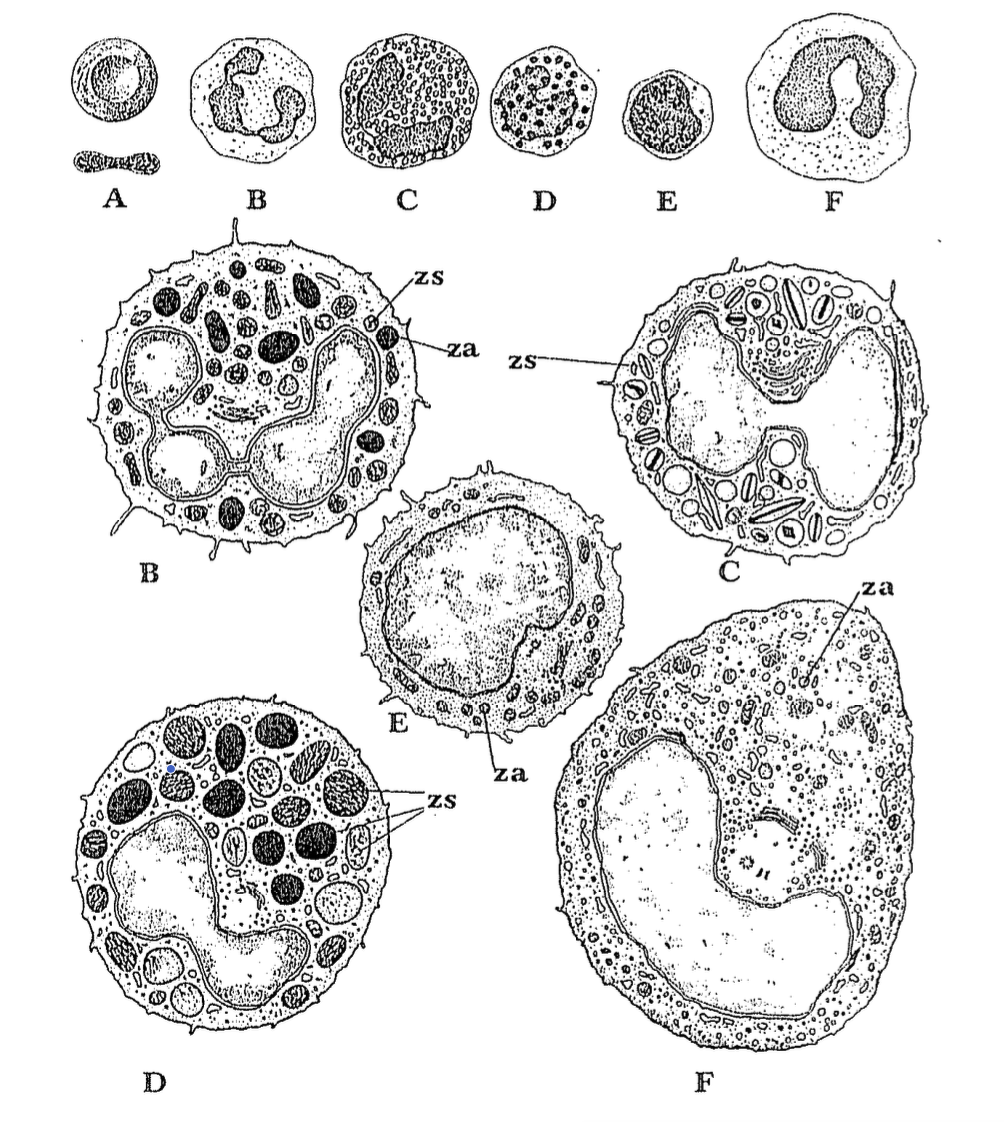
\includegraphics[width=0.8\textwidth]{morfotyczne}
    \caption{Elementy morfotyczne krwi w obrazie mikroskopu optycznego i elektronowego. Rysunek pochodzi z “Kompendium histologii“ autorstwa Tadeusza Cichockiego, Jana Litwina i Jadwigi Mireckiej \cite{histology}.}
    \label{fig:electron_microscope}
\end{figure}

Rozwój metod komputerowej klasyfikacji komórek jest bardzo istotny, ponieważ potencjalne zautomatyzowanie procesu zliczania komórek pozwoliłoby na szybsze stawianie diagnozy i zaoszczędzenie wielu godzin pracy diagnostów.

Obecne rozwiązania służące do opisu komórek w krwi lub szpiku kostnym bazują na cytometrii przepływowej (czyli analizie kąta odbicia fali światła).
Warto natomiast zwrócić uwagę na to, że zdjęcie komórki (to znaczy obrazowanie w zakresie światła widzialnego) jest wystarczające do rozpoznania typu komórki przez człowieka, a więc niesie dostateczną ilość informacji.
\textcolor{red}{Oznacza to, że istnieją przesłanki, że} odpowiednio zaawansowany model sztucznej inteligencji byłby w stanie klasyfikować komórki jedynie na podstawie wizji komputerowej, bez potrzeby analizy widma falowego lub kątów odbicia światła.


\section{Algorytmy widzenia komputerowego}

W niniejszym projekcie, oprócz widzenia komputerowego realizowanego przez splotowe sieci neuronowe, wykorzystano również inne algorytmy do analizy obrazów.
Jednym z nich jest mechanizm \textbf{progowania obrazu} (z ang. \textit{thresholding}).
Operacja ta przyporządkowuje wartość maksymalną piksela na obrazie wyjściowym, gdy poziom jasności na obrazie wejściowym jest większy od zadanego progu $k$.
Analogicznie, wyjściowy piksel przyjmuje wartość minimalną (najczęściej $0$), gdy piksel wejściowy jest poniżej progu $k$ lub wartość jest równa (zob.
równanie~\ref{eq:thresholding}).

\begin{equation}
    T(x, y) =
    \begin{cases}
        0 & \text{jeśli } I(x, y) < k \\
        1 & \text{jeśli } I(x, y) \geq k
    \end{cases}\label{eq:thresholding}
\end{equation}

Inną ważną metodą widzenia komputerowego są \textbf{momenty Hu} (zwane też momentami obrazów).
Momenty Hu to zestaw metryk służących do opisu kształtu i właściwości pewnego regionu obrazu~\cite{vision}.
Korzystają one z analizy rozkładu jasności pikseli w obrazie.
W algorytmie ekstrakcji obrazów komórek z dużego zdjęcia rozmazu wykorzystywane są momenty centralne do wyznaczania punktów centralnych komórek.
Wzór na tak zwany moment centralny $\mu_{ij}$ przedstawia równanie~\ref{eq:central_moment}, zaś współrzędne punktu centralnego można wyznaczyć korzystając z równań~\ref{eq:centroid}.

\begin{equation}
    \mu_{ij} = \sum_x \sum_y x^i y^j I(x, y)\label{eq:central_moment}
\end{equation}

\begin{equation}
    \bar{x} = \frac{M_{10}}{M_{00}}, \quad \bar{y} = \frac{M_{01}}{M_{00}}\label{eq:centroid}
\end{equation}


\section{GradCAM - wytłumaczalne uczenie maszynowe}

GradCAM (z ang. \textit{Gradient-weighted Class Activation Mapping}) to technika, która umożliwia użytkownikom splotowych sieci neuronowych lepsze zrozumienie procesu podejmowania decyzji przez model uczenia maszynowego.
Jest to jedna z podstawowych metod zagadnienia wytłumaczalnego SI (z ang. \texit{explainable artificial intelligence}).
Po wykonaniu przejścia w przód sieci neuronowej GradCAM jest w stanie wygenerować mapę cieplną wskazującą obszary obrazu, które były istotne do podjęcia decyzji przez model.
Zasada działania algorytmu GradCAM:
\begin{itemize}
    \item Przejście w przód i propagacja wsteczna.
    Ten krok ma za zadanie obliczyć gradient $\pd{{y^c}}{{A^k}}$, gdzie $A^k$ jest $k$-tą mapą cech w ostatniej warstwie splotowej.
    \item Uśrednianie gradientów po wymiarach mapy cech, w celu uzyskania wag $a^c_k$ dla każdej mapy cech $k$ (zob.
    równanie~\ref{eq:gradcam_averaging}).
    \begin{equation}
        a^c_k = \frac{1}{Z} \sum_i \sum_j \pd{{y^c}}{{A^k_{ij}}}\label{eq:gradcam_averaging}
    \end{equation}
    \item Obliczenie ważonej mapy cech.
    Ostateczna mapa cieplna jest wyliczana jako kombinacja liniowa mapy aktywacji i wag $a^c_k$ (zob.
    równania~\ref{eq:gradcam_final} i~\ref{eq:relu}).
    \begin{equation}
        L^c_{\text{gradcam}} = \text{ReLU} \left( \sum_k \alpha^c_k A^k \right)\label{eq:gradcam_final}
    \end{equation}
    \begin{equation}
        \text{ReLU}(x) = \max(0, x).\label{eq:relu}
    \end{equation}
    \item Interpolacja do rozmiaru obrazu wejściowego-obliczona mapa cech $L^c_{\text{gradcam}}$ jest skalowana, by można było nałożyć ją na obraz wejściowy.
\end{itemize}

Skorzystanie z metod wytłumaczalnego uczenia maszynowego pozwala na zwiększenie transparentności modelu i lepsze zrozumienie procesu podejmowania decyzji.
Jest to szczególne ważne z punktu widzenia zastosowań sieci neuronowych w medycynie, ponieważ lekarz może dogłębniej przyjrzeć się przesłankom, co stoi za daną odpowiedzią modelu.
W przypadku zadania rozpoznawania rodzajów komórek z krwi obwodowej bądź szpiku mapa cieplna GradCAM wskazuje na te obszary komórki, po których można rozpoznać jej typ.
Innym przykładem zastosowania wytłumaczalnego uczenia maszynowego jest rozpoznawanie zmian nowotworowych na skanach mózgu z rezonansu magnetycznego.
Algorytm GradCAM może wskazać obszar na skanie, po którym model stwierdził obecność nowotworu~\cite{gradcam_brain_tumor}.
    \chapter{Realizacja projektu}


\section{Wykorzystane technologie}

\subsection{Język programowania Python}

Kod projektu został napisany w języku Python. Wybór tego języka był spowodowany szeroką dostępnością bibliotek i
narzędzi wspomagających uczenie maszynowe. W szczególności należy zwrócić uwagę na biblioteki \textit{PyTorch} (użyta w projekcie) oraz \textit{Tensorflow} (alternatywa).
Są to dwie najpopularniejsze biblioteki do operowania na tensorach (tensor to uogólnienie macierzy na wiele wymiarów).
Obie pozwalają na przyśpieszanie obliczeń z użyciem zewnętrznych akceleratorów takich jak np. karty graficzne.

Podczas prac badawczych, wykorzystana wersja Pythona to \textit{3.12.0}.

\subsection{Biblioteka PyTorch}

Biblioteka PyTorch jest obecnie najpopularniejszą biblioteką uczenia maszynowego.
Pozwala ona projektować obliczenia w formie modułów i posiada silnik automatycznego różniczkowania grafu obliczeniowego (z ang. \textit{autograd}).
Owy silnik jest kluczowy z perspektywy trenowania sieci neuronowych, ponieważ jest w stanie optymalizować parametry modelu.
Warto zwrócić uwagę na to, że PyTorch stawia nacisk na przejrzystość obliczeń - dla porównania operacje w Tensorflow są nierzadko
ukryte pod gotowymi funkcjami (zob. listing~\ref{lst:tensorflow_sample} i~\ref{lst:pytorch_sample})

\begin{lstlisting}[language=ipython,caption={Przykładowa sieć neuronowa w Tensorflow},label={lst:tensorflow_sample}]
tensorflow_model = tf.keras.Sequential([
    tf.keras.layers.Flatten(input_shape=(28, 28)),
    tf.keras.layers.Dense(128, activation='relu'),
    tf.keras.layers.Dense(10, activation='softmax')
])

tensorflow_model.compile() # Brak doglebnej kontroli nad przeplywem obliczen
\end{lstlisting}


\begin{lstlisting}[language=ipython,caption={Przykładowa sieć neuronowa w PyTorch},label={lst:pytorch_sample}]
class PyTorchNetwork(nn.Module):
    def __init__(self):
        super(Net, self).__init__()
        self.flatten = nn.Flatten()
        self.fc1 = nn.Linear(28 * 28, 128)
        self.relu = nn.ReLU()
        self.fc2 = nn.Linear(128, 10)

    def forward(self, x): # Dokladna kontrola nad przeplywem obliczen
        x = self.flatten(x)
        x = self.fc1(x)
        x = self.relu(x)
        x = self.fc2(x)
        return x
\end{lstlisting}

PyTorch oferuje również zestaw narzędzi do przetwarzania danych, dostarcza również gotowe, pretrenowane modele dla najpopularniejszych architektur.
Przykładami są pakiety \textit{torchvision} lub \textit{torch.utils}. Biblioteka jest w stanie wykorzystywać karty graficzne (z ang. \textit{graphical processing unit, GPU}) do przyspieszania obliczeń.

\subsection{Biblioteka OpenCV}

Biblioteka OpenCV \cite{opencv} dostarcza implementacje wielu algorytmów wizji komputerowej.
OpenCV \textcolor{red}{zawiera} interfejs programistyczny, dzięki któremu programista Pythona może komunikować się z implementacją algorytmów w C++.
To zapewnia szybkość wykonywania obliczeń, jednocześnie nie wymuszając na programiście pisania kodu w C++. Przykład wykorzystania biblioteki OpenCV widoczny jest na listingu \ref{lst:opencv_sample}
- kod wylicza momenty Hu.

OpenCV w niniejszym projekcie jest wykorzystywane do automatycznej ekstrakcji obrazów z komórkami na podstawie dużego zdjęcia spod mikroskopu.
Więcej informacji na ten temat znajduje się w rozdziale \ref{sec:kwadraty}.

\begin{lstlisting}[language=ipython,caption={Obliczenie momentów Hu z użyciem OpenCV}, label={lst:opencv_sample}]
import cv2

image = cv2.imread('obraz.jpg', 0)  # 0 oznacza wczytanie obrazu w odcieniach szarosci

hu_moments = cv2.HuMoments(cv2.moments(image)).flatten()

print("Momenty Hu:")
for i in range(0, 7):
    print(f"Moment {i+1}: {hu_moments[i]}")
\end{lstlisting}

\subsection{Inne narzędzia}

Kod źródłowy projektu jest przechowywany w repozytorium na platformie GitHub (dostępny pod adresem \url{https://github.com/matisiekpl/thesis}).
Wykresy były generowane za pomocą biblioteki \textit{matplotlib} \cite{matplotlib},
a metryki liczone z użyciem funkcji pakietu \textit{scikit-learn} \cite{scikit_learn}.

\subsection{Sprzęt}

Do prac badawczych został użyty Apple Macbook Pro 2020 (M1/16GB pamięci).
Trenowanie sieci odbywało się na platformie \textit{kaggle.com}, która oferuje bezpłatne 30 godzin obliczeń co miesiąc z kartą graficzną \textit{NVIDIA P100}.


\section{Zbiór danych}

Wykorzystany w projekcie zbiór danych to kolekcja 170 tysięcy zdjęć komórek z rozmazów szpiku kostnego.
Zdjęcia mają nadane etykiety przez diagnostów i przedstawiają różne komórki widziane pod mikroskopem.
Próbki szpiku kostnego pochodzą z biopsji 945 pacjentów z Monachijskiego Labolatorium Białaczek (\textit{MLL Münchner Leukämielabor} \cite{mll}).
Akwizycja obrazu polegała na wykonaniu zdjęcia mikroskopią Brightfield'a~\cite{microscopy} z 40-krotnym powiększeniem.
Producentem mikroskopu było przedsiębiorstwo Fraunhofer IIS.

\begin{figure}
    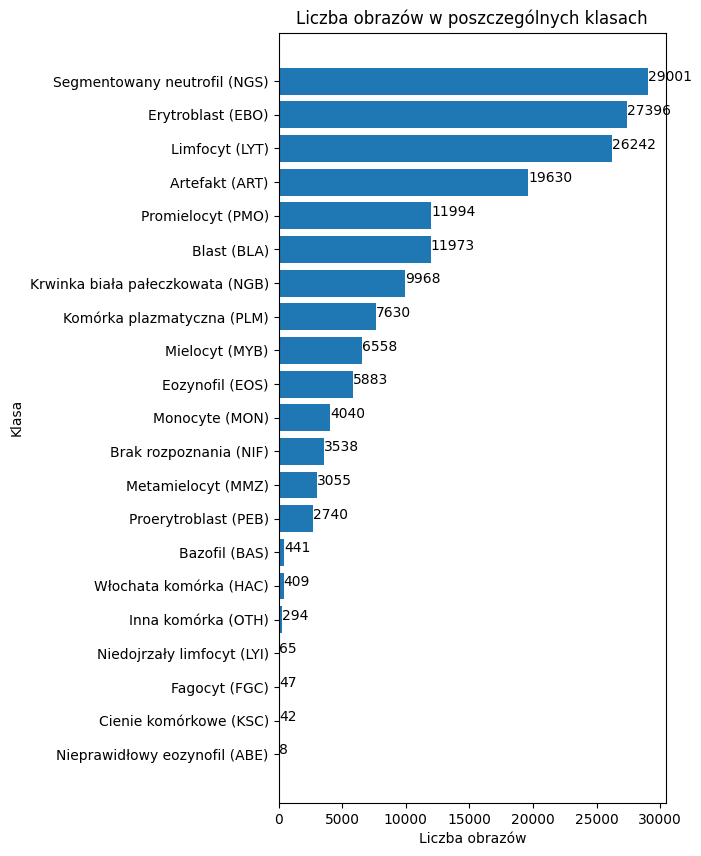
\includegraphics[width=\textwidth]{images_count}
    \caption{Histogram rozkładu próbek w klasach w zbiorze danych}
    \label{fig:images_count_vis}
\end{figure}

\begin{figure}
    \centering
    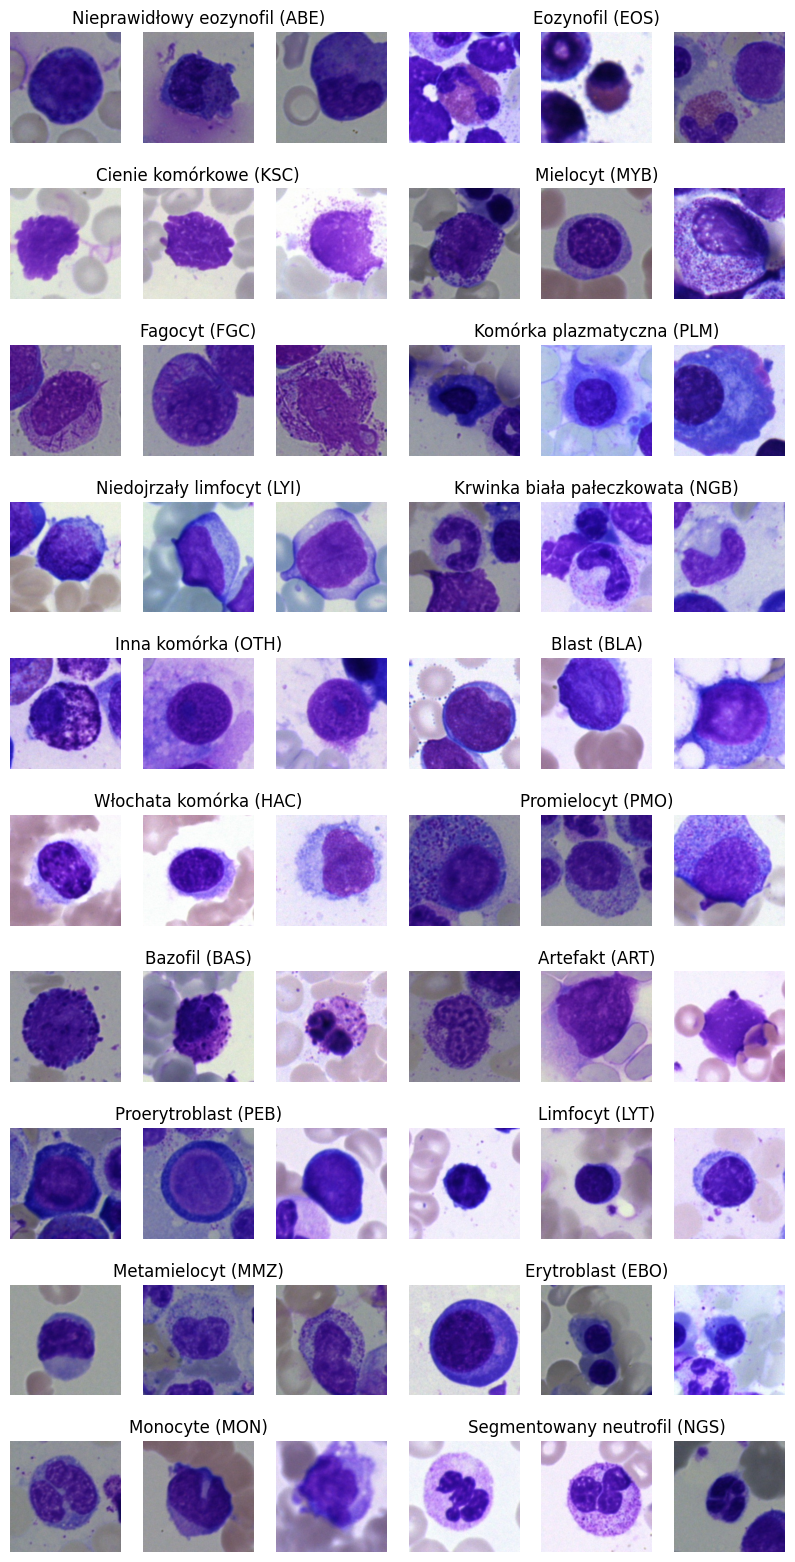
\includegraphics[height=0.9\textheight]{images_examples}
    \caption{Przykładowe zdjęcia komórek ze zbioru danych dla każdej z klas}
    \label{fig:images_examples}
\end{figure}

Komórki były barwione metodą Maya-Grünwalda-Giemsa \cite{histology}.
Zbiór danych zawiera 21 klas, lecz w trakcie trenowania sieci neuronowych wykorzystano jedynie 11 (odrzucone klasy posiadały bardzo małą ilość próbek).
Histogram rozkładu klas jest widoczny na rys. \ref{fig:images_count_vis}.
Zbiór danych jest niezrównoważony, ponieważ ilość obrazów w każdej klasie znacząco się różni.
Przykładowe zdjęcia są widoczne na rys \ref{fig:images_examples}.


\section{Struktura projektu}

\subsection{Przygotowanie danych}

Zbiór danych to katalog ze zdjęciami.
Zdjęcia są pogrupowane w podkatalogach, gdzie jego nazwa oznacza typ komórki.
Każdy podkatalog zawiera kolorowe zdjęcia w formacie \textit{.jpg} w rozmiarze \textit{250 pikseli x 250 pikseli}.
Przed treningiem sieci neuronowej konieczne jest przetwarzanie wstępne zbioru danych (z ang. \textit{preprocessing}).

\begin{lstlisting}[language=ipython,caption={Transformacja danych}, label={lst:transforms}]
transform = transforms.Compose([
    transforms.Resize((224, 224)), # przeskaluj obrazy
    transforms.RandomEqualize(1), # wyrownaj histogram z prawdopodobienstwem 1, czyli dla kazdego obrazu
    transforms.ToTensor(), # zamien na Tensor
    transforms.Normalize(mean=[0.485, 0.456, 0.406], std=[
        0.229, 0.224, 0.225]), # normalizuj wedlug mediany i odch. stand.
])
\end{lstlisting}

Do realizacji przygotowania danych wykorzystano pakiet \textit{torchvision.transforms}.
Kod transformacji jest przedstawiony na listingu~\ref{lst:transforms}.
Wykonuje on przeskalowanie obrazu wejściowego do rozmiaru \textit{224 piksele na 224 piksele}.
Następnie wyrównuje histogram i normalizuje według średniej i odchylenia standardowego (rys.~\ref{fig:transformations_example}).

Wyrównanie histogramu jest konieczne z powodu różnic w odcieniach barwienia Maya-Grünwalda-Giemsa~\cite{stain}.
Przy każdym wykonaniu rozmazu intensywność kolorów komórek jest inna.
Taka normalizacja zapobiega błędnemu nauczeniu się sieci neuronowej ze względu na odcień, a nie kształt i wygląd komórek.

\begin{figure}
    \centering
    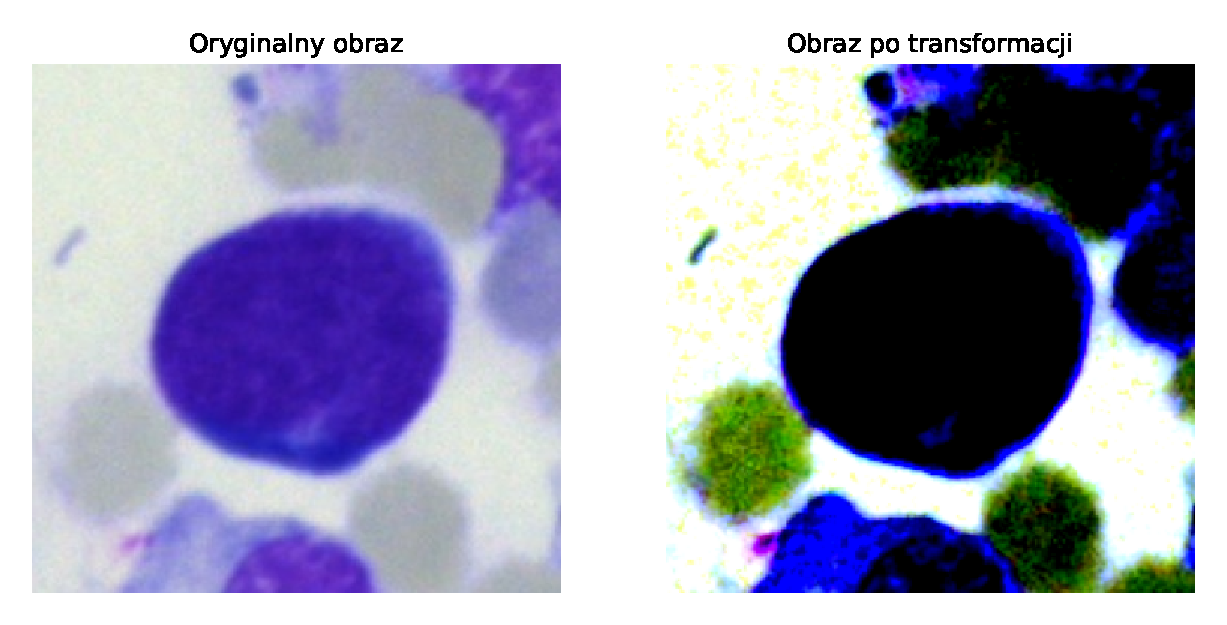
\includegraphics[width=\textwidth]{image_transform}
    \caption{Porównanie obrazu wejściowego przed i po transformacji}
    \label{fig:transformations_example}
\end{figure}

Po przetwarzaniu zbiór danych został podzielony losowo na zestaw treningowy i walidacyjny w proporcjach odpowiednio \textit{80:20}.
Zestaw treningowy służy do optymalizacji parametrów sieci neuronowej.
Zestaw walidacyjny natomiast jest używany do sprawdzania jakości modelu na obrazach, których sieć neuronowa "nigdy nie widziała".

\subsection{Trening sieci neuronowej}

Niniejsza praca ma za zadanie między innymi porównać różne architektury splotowych sieci neuronowych i ocenić,
która z nich wypada najlepiej w zadaniu klasyfikacji komórek z rozmazów szpiku kostnego.
Omówiony poniżej trening sieci neuronowej o architekturze \textit{EfficientNet B0} wygląda tak samo dla innych architektur, takich jak \textit{EfficientNet B5}, \textit{ResNet} i innych.
Współczynnik uczenia wynosił \textit{0.001}, a ilość epok była równa 3.
\textcolor{red}{Niestety z powodu ograniczeń infrastruktury do trenowania, nie udało się wykonać walidacji krzyżowej dla każdego z modeli osobno. Zbiór walidacyjny był natomiast wybierany losowo za każdym razem, gdy badano nową sieć neuronową.}

Trenowanie sieci neuronowej z użyciem biblioteki PyTorch sprowadza się do iterowania po zbiorze wejściowym i wykonywania kroku optymalizacyjnego przy każdym przejściu.
Uproszczony schemat działania głównej pętli treningowej (kod przestawiony na listingu~\ref{lst:train}):

\begin{enumerate}
    \item Pobranie miniwsadu z próbkami treningowymi i skopiowanie ich na urządzenie zewnętrzne, czyli kartę graficzną.
    \item Wykonanie przejścia w przód sieci neuronowej.
    Oznacza to obliczenie wartości neuron na warstwie wyjściowej na bazie uprzednio pobranych próbek.
    \item Porównanie wyjścia sieci neuronowej z oczekiwanymi predykcjami i obliczenie błędu sieci.
    \item Obliczenie gradientów za pomocą algorytmu propagacji wstecznej.
    \item Wykonanie kroku optymalizacyjnego z użyciem optymalizatora \textit{Adam}.
    \item Obliczenie metryk dla zbioru walidacyjnego i zapisanie ich.
\end{enumerate}

\lstinputlisting[label={lst:train}, caption={Kod pętli treningowej w języku Python z wykorzystaniem PyTorch}, language=ipython]{train.py}

\subsection{Ewaluacja jakości modelu}

\begin{figure}
    \centering
    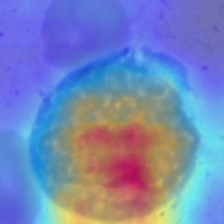
\includegraphics[width=0.5\textwidth]{cam}
    \caption{Mapa cieplna GradCAM dla obrazu komórki plazmatycznej}
    \label{fig:cam}
\end{figure}


Wyjściem modelu jest rozkład prawdopodobieństwa rozpoznania poszczególnych rodzajów komórek oraz mapa cieplna GradCAM.
Przykładowa mapa cieplna jest widoczna na rys.~\ref{fig:cam}.
Przedstawia ona miejsca na obrazie, które najbardziej wpłynęły na predykcję.
\textcolor{green}{
    Zgadzają się one z obszarami, na które zwraca uwagę lekarz - sprawdza on wygląd jądra komórkowego jak i jego ziarnistości.
}

Do sprawdzenia jakości modelu uczenia maszynowego konieczny jest dobór właściwych metryk.
Ze względu na to, że trenowany jest klasyfikator wieloklasowy, a zbiór danych nie jest zrównoważony, zwykłe metryki takie jak dokładność (z ang. \textit{accuracy}) nie wystarczą.
Dla każdej klasy jest liczona precyzja (z ang. \textit{precision}) i czułość (z ang. \textit{recall}).
Obie te metryki składają się do obliczenia wyniku F1 (z ang. \textit{F1-score})~\cite{geron}.
Co ważne, wynik F1 jest liczony z uwzględnieniem wag poszczególnych klas.
Obliczana jest również macierz pomyłek.
Informuje ona o tym, które klasy są najczęściej mylone między sobą.
Metryki są zapisywane do pliku tekstowego oraz do plików obrazów w celu późniejszej analizy.


\section{Interfejs użytkownika}

W celu łatwego korzystania z modelu uczenia maszynowego przez diagnostów \textcolor{red}{opracowana została} aplikacja internetowa do interakcji z nim.
Zrzut ekranu interfejsu użytkownika jest widoczny na rys.~\ref{fig:ui}.
Aplikacja została napisana z użyciem \textit{Vue}~\cite{vue} - biblioteki do tworzenia interaktywnych interfejsów użytkownika dla sieci web.
Łączy się ona z serwerem HTTP napisanym z użyciem biblioteki Flask~\cite{flask}.
Serwer eksponuje interfejs REST API, który dla wysłanego zdjęcia zwraca rozkład prawdopodobieństwa \textcolor{red}{ rozpoznania poszczególnych klas}.
Przed wywołaniem modelu, funkcja upewnia się, że przychodzący obrazek jest poprawnego formatu.
Dopiero po zwalidowaniu poprawności danych, kod przystępuje do utworzenia rozkładu prawdopodobieństwa (zmienna \textit{result}).
Renderowana jest również mapa cieplna GradCAM informująca użytkownika o regionach obrazu, które były kluczowe dla modelu w trakcie wykonywania predykcji.


\begin{figure}
    \centering
    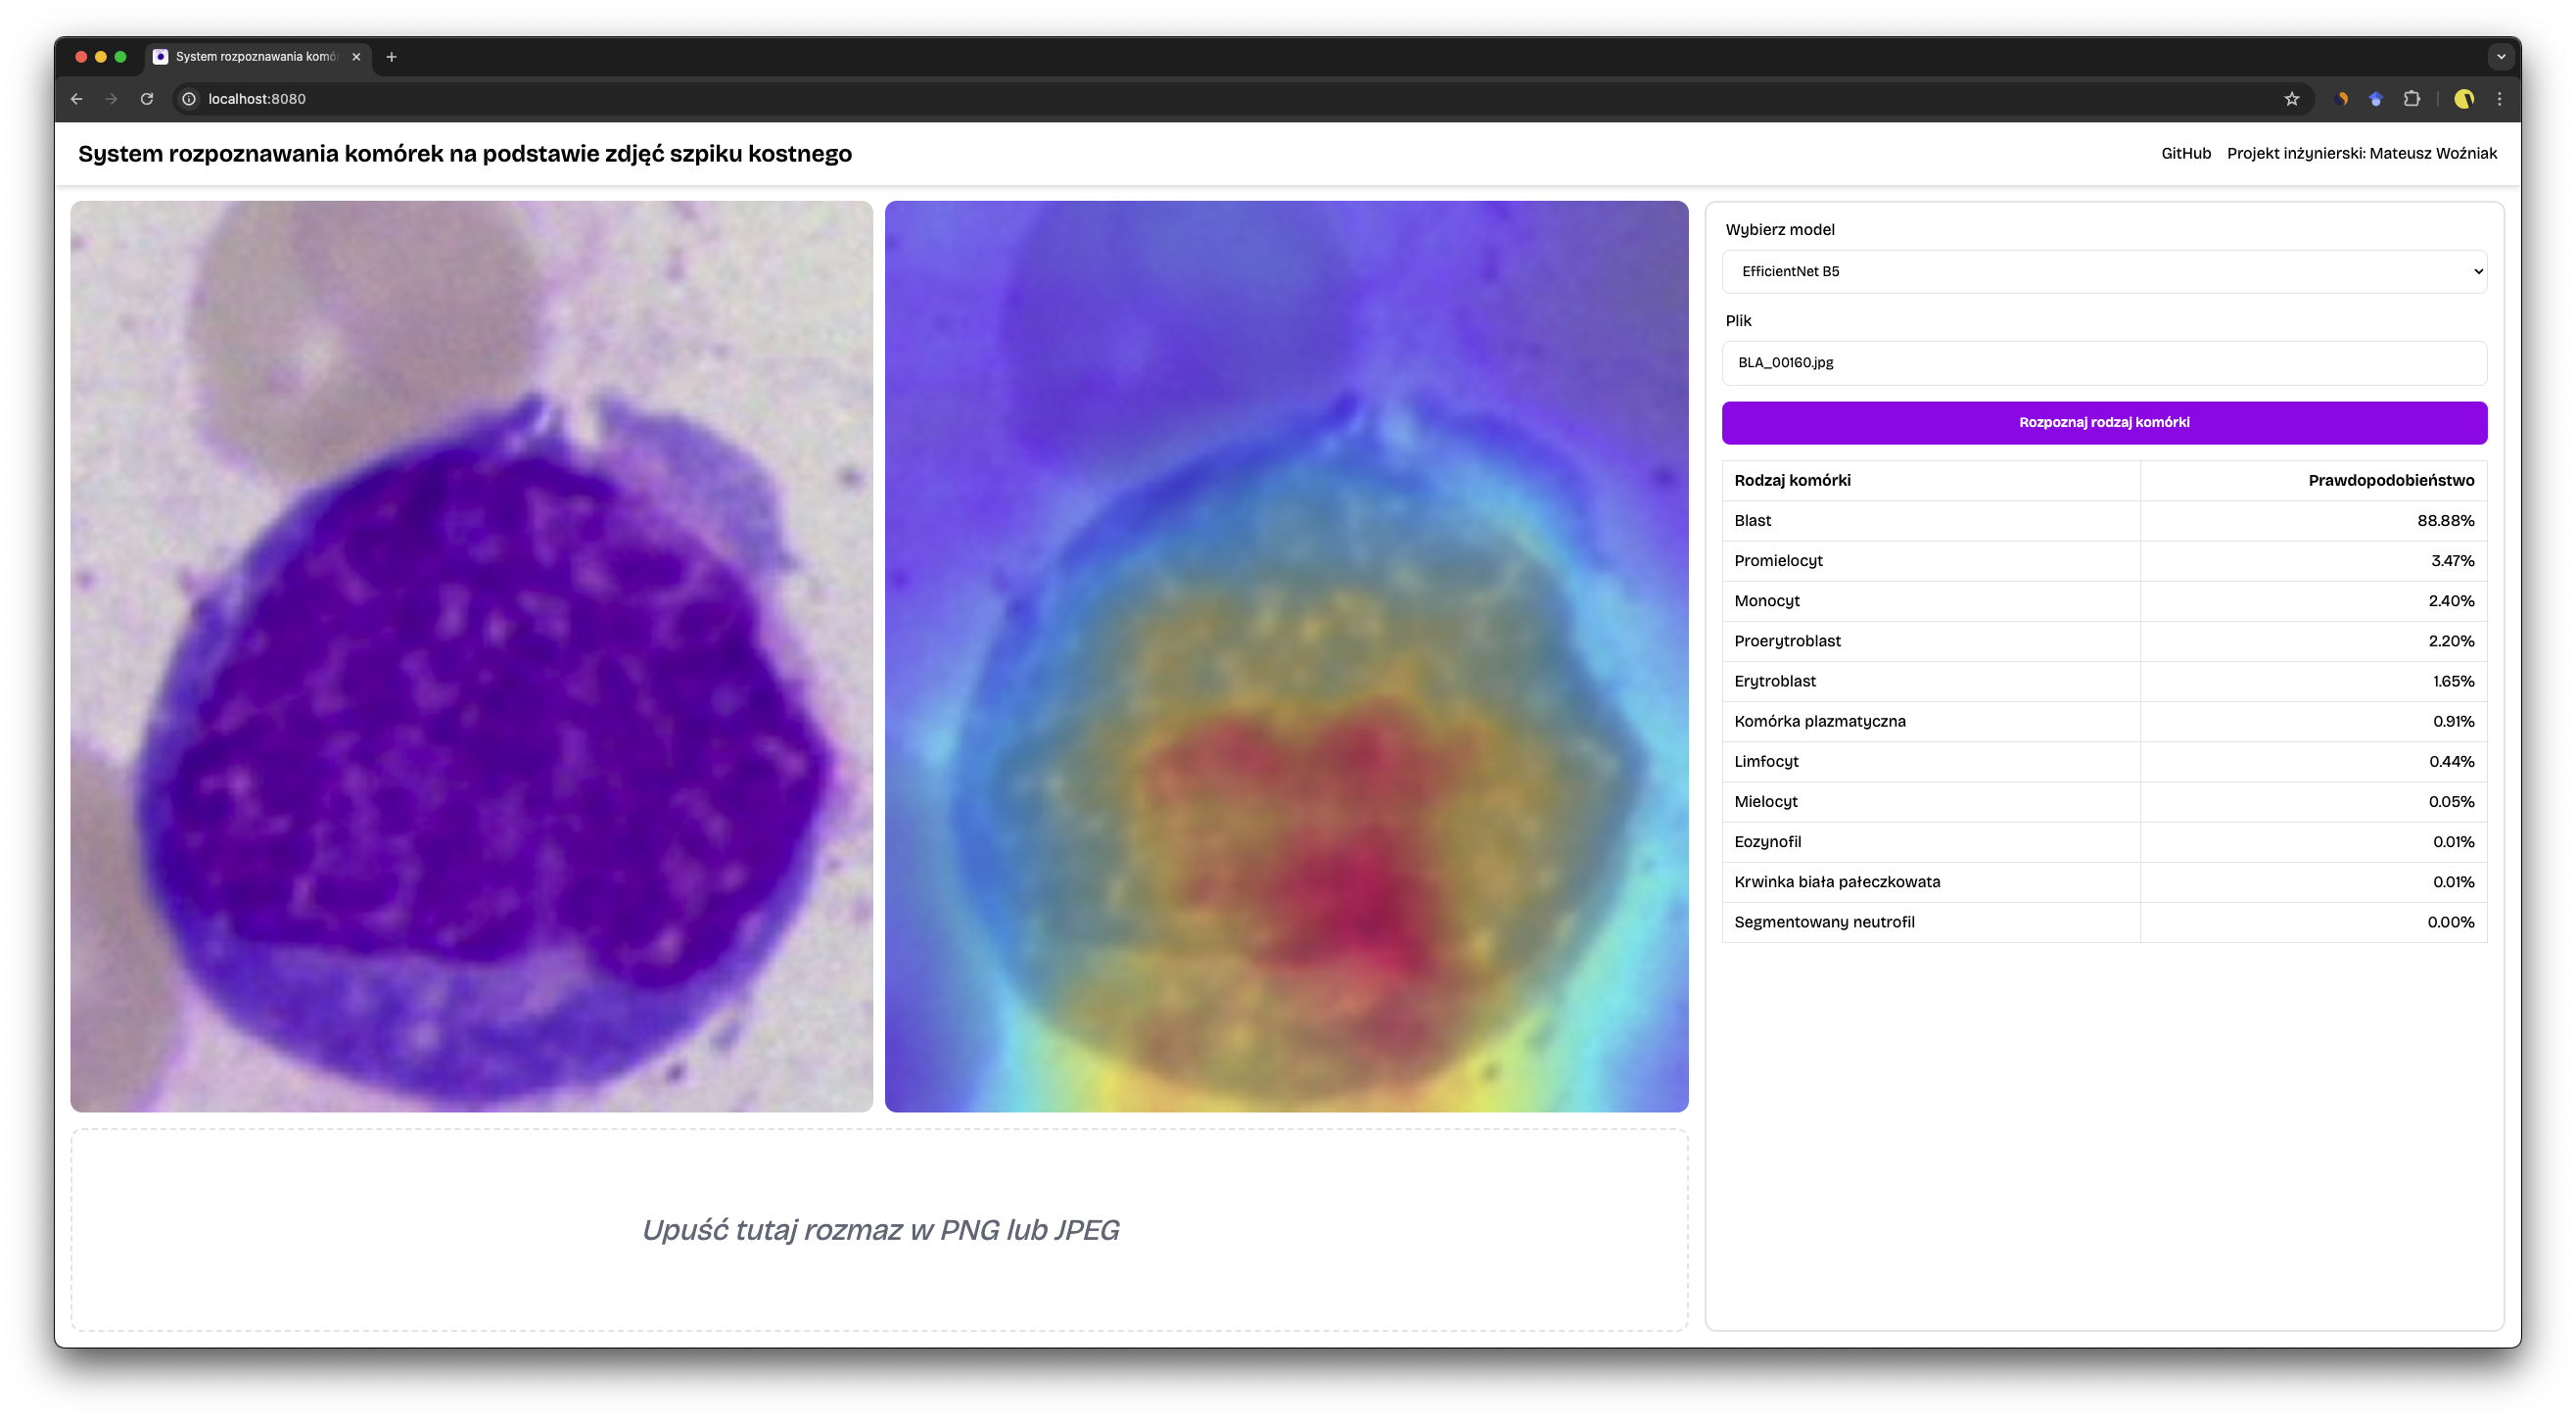
\includegraphics[width=\textwidth]{app}
    \caption{Aplikacja internetowa do rozpoznawania komórek}
    \label{fig:ui}
\end{figure}


\begin{figure}
    \centering
    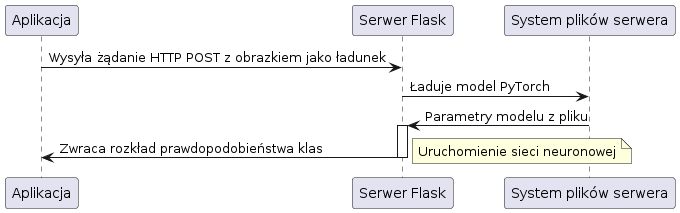
\includegraphics[width=0.8\textwidth]{arch}
    \caption{Architektura klient-serwer aplikacji internetowej i serwera Flask}
    \label{fig:arch}
\end{figure}

By skorzystać z aplikacji internetowej, należy przeciągnąć plik ze zdjęciem komórki do sekcji "Upuść tutaj rozmaz w PNG lub JPEG".
Po wysłaniu obrazu użytkownik może wybrać model i kliknąć przycisk "Rozpoznaj rodzaj komórki".
Następnie ukaże się tabela z rozkładem prawdopodobieństwa (po prawej stronie okna).
Stylizowanie aplikacji zostało wykonane z użyciem biblioteki CSS o nazwie \textit{Tailwind.css}~\cite{tailwind}.
Komunikacja klient-serwer jest zapewniona przez bibliotekę \textit{Axios}~\cite{axios}.
Architekturę przedstawia rys.~\ref{fig:arch}.


\section{Algorytm ekstrakcji obrazów komórek z dużego zdjęcia rozmazu}\label{sec:kwadraty}

Zbiór danych użyty w trakcie trenowania splotowej sieci neuronowej przedstawia komórki, które zajmują prawie całą cześć obrazu.
Innymi słowy, każdy obrazek stanowi wycinek dużego skanu z rozmazu.
Często jednak istnieje potrzeba zautomatyzowania procesu wycinania kwadratowych obrazów przedstawiających komórki z dużego skanu.
Zaproponowano algorytm korzystający z różnych metod wizji komputerowej do osiągnięcia tego zadania.

Niniejszy algorytm przyjmuje obraz przedstawiający kilkanaście komórek różnego rodzaju i eksportuje
każdą komórkę do kwadratowego zdjęcia.
Algorytm wykonuje następujące kroki w celu wyznaczenia komórek z obrazka:

\begin{figure}
    \centering
    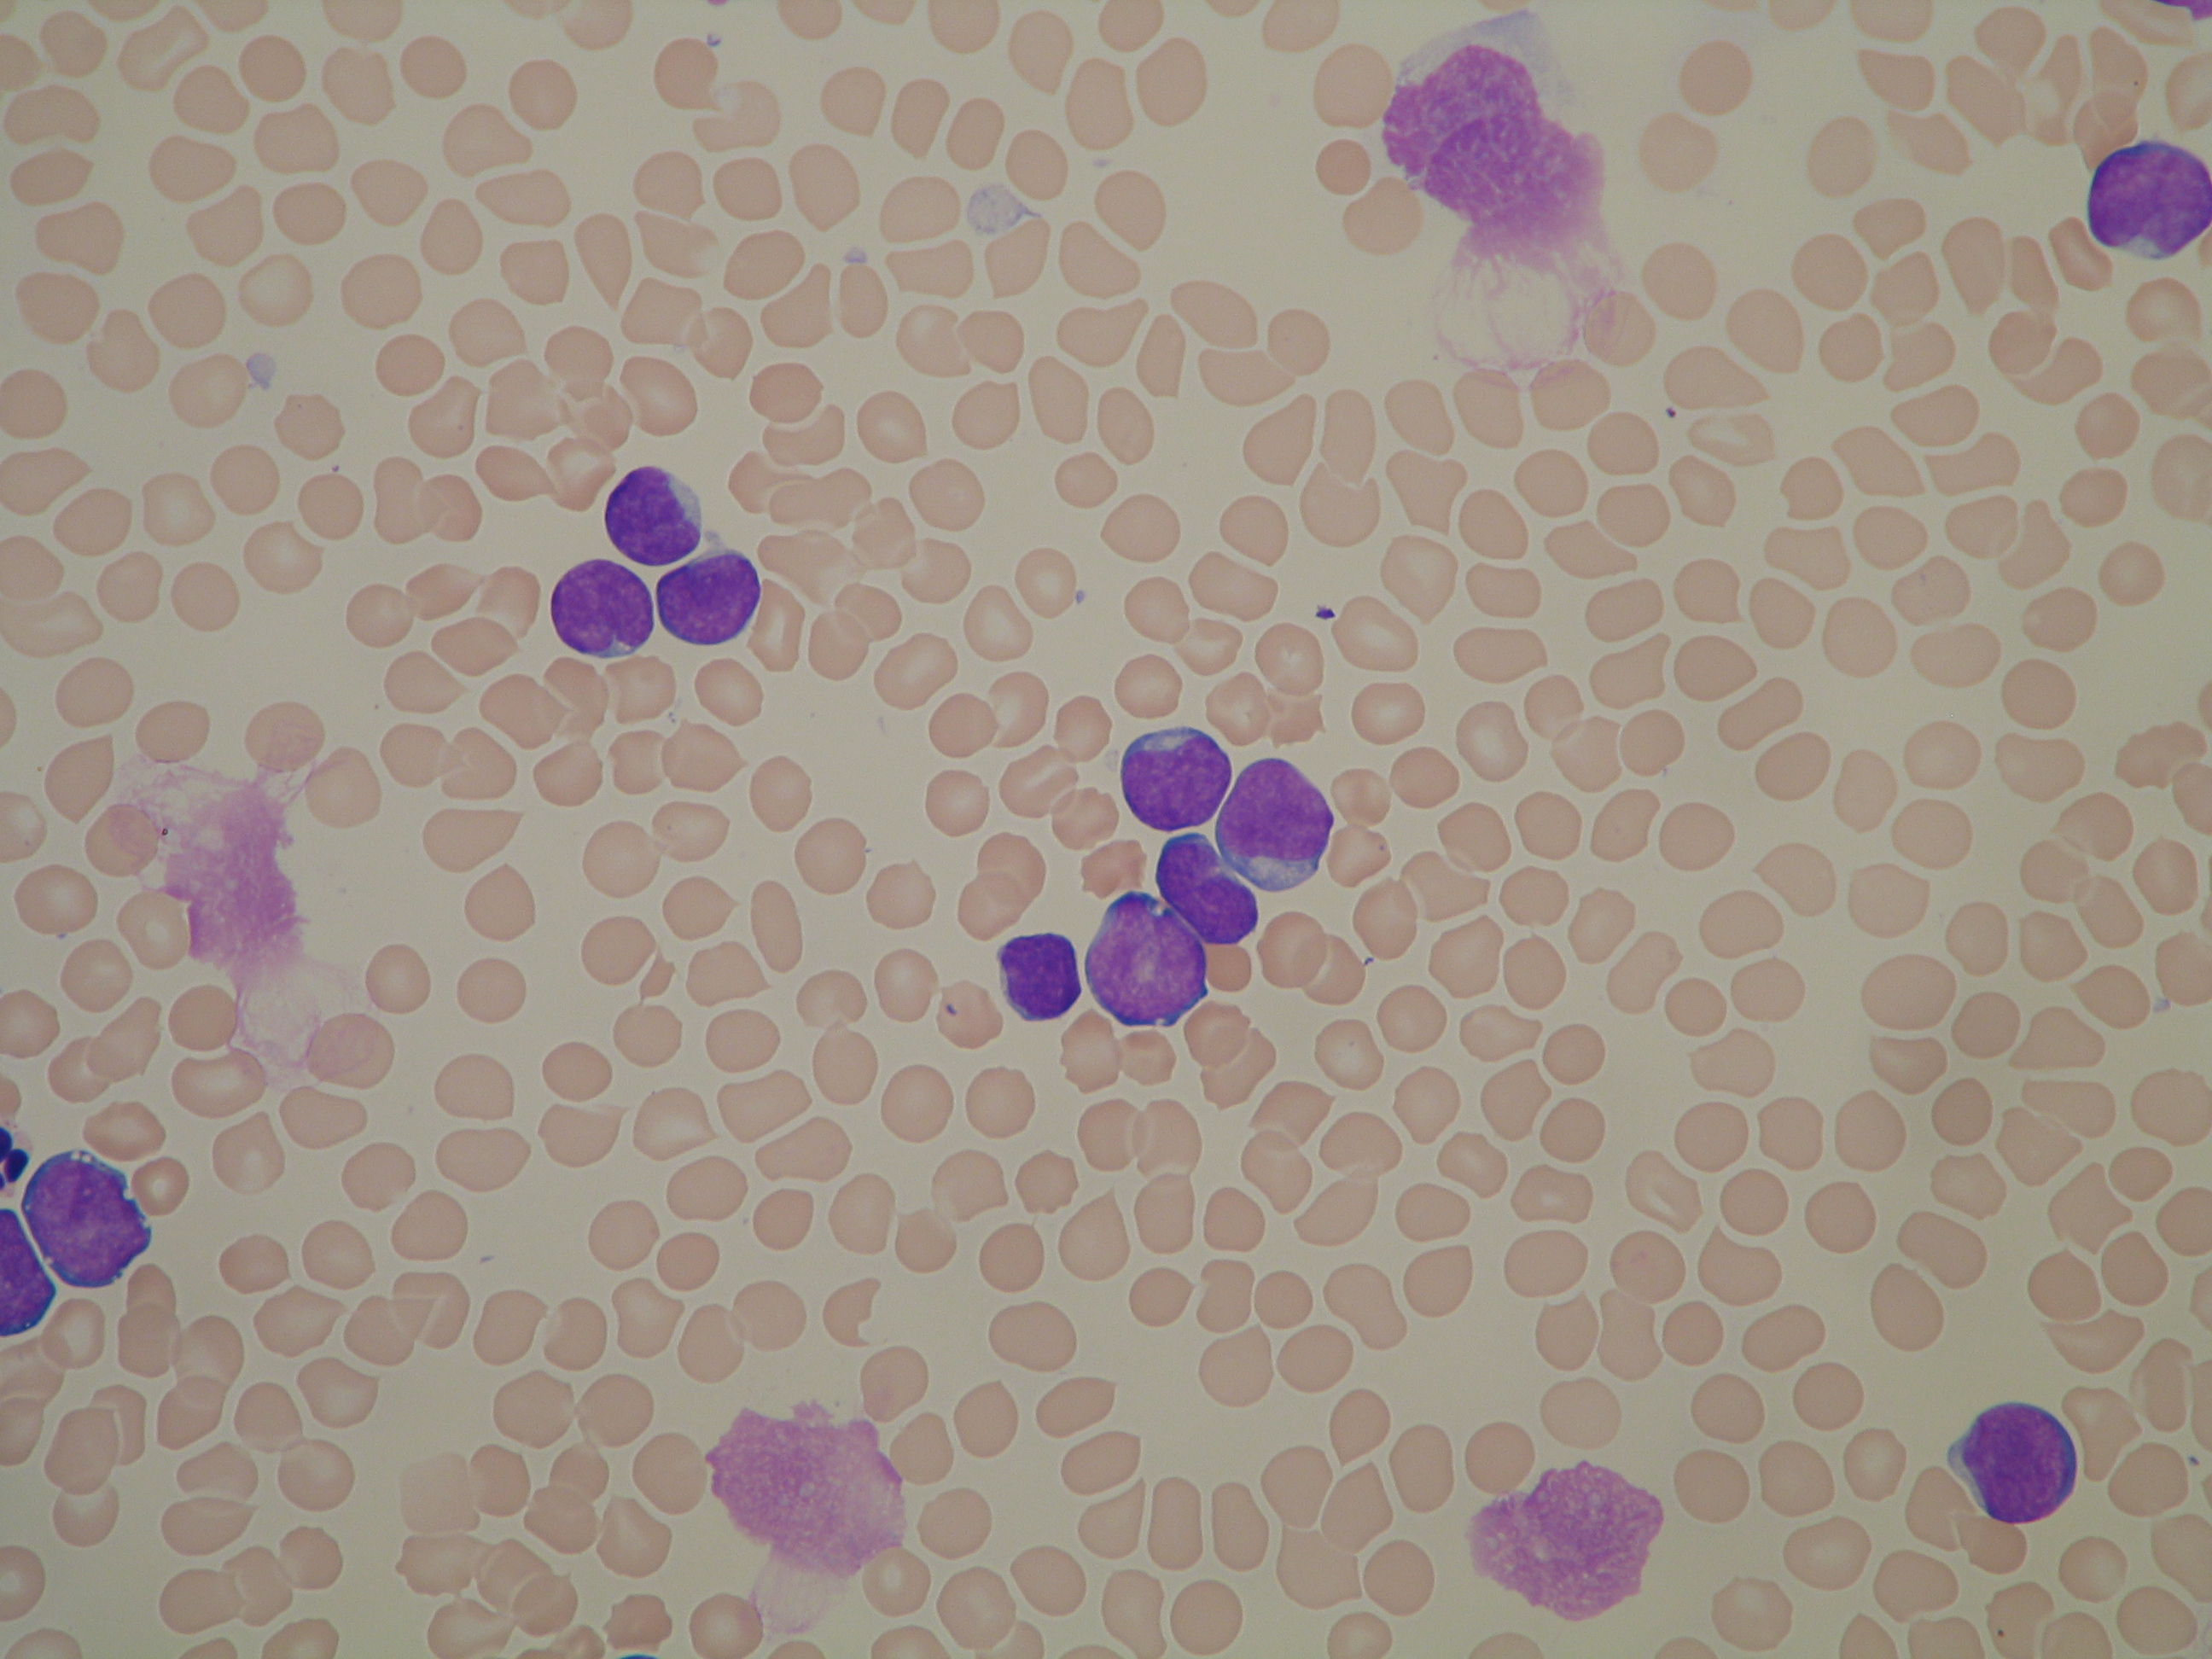
\includegraphics[width=0.8\textwidth]{Im060_1}
    \caption{Wejście algorytmu}
    \label{fig:extract_input}
\end{figure}

\begin{figure}
    \centering
    
\includegraphics[width=0.8\textwidth]{Im060_1_thresh}
    \caption{Obrazek po progowaniu}
    \label{fig:extract_thresh}
\end{figure}

\begin{figure}
    \centering
    \includegraphics[width=0.8\textwidth]{Im060_1_contours}
    \caption{Oznaczone kontury wraz z punktami centralnymi}
    \label{fig:extract_contours}
\end{figure}

\begin{figure}
    \centering
    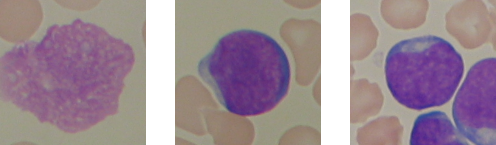
\includegraphics[width=0.8\textwidth]{cells}
    \caption{Wyekstraktowane kwadratowe obrazki}
    \label{fig:extract_squares}
\end{figure}

\begin{enumerate}
    \item Konwersja oryginalnego obrazu (rys.~\ref{fig:extract_input}) na skalę szarości.
    Jest to konieczne, ponieważ progowanie w kroku drugim nie może odbywać się na obrazie kolorowym.
    Do konwersji zastosowano funkcję \textit{cv2.cvtColor} - pozwala ona konwertować obraz z jednej przestrzeni kolorów do innej.
    \item Progowanie z pomocą algorytmu Otsu~\cite{otsu}.
    Jest to algorytm adaptacyjnego progowania, często stosowany do analizy obrazów medycznych.
    Progowanie ma na celu wyodrębnienie ciemniejszych obszarów obrazu - cytoplazmy i jądra komórek (rys.~\ref{fig:extract_thresh}). Otsu jest algorytmem progowania globalnego i opiera się na analizie histogramu.
    Dąży on do maksymalizacji wariancji międzyklasowej.
    \item Wyznaczenie konturów z pomocą funkcji \textit{cv2.findContours}~\cite{contours}.
    Kontur jest definiowany jako pewna ciągła krzywa, która łączy punkty o tej samej intensywności.
    W opisanym algorytmie kontury mają za zadanie informować o granicach komórki.
    Argumentem funkcji jest flaga \textit{cv2.RETR\_EXTERNAL}, która powoduje, że zwrócone zostają jedynie najbardziej zewnętrzne kontury - kontury wewnętrzne są ignorowane.
    \item Obliczanie punktów centralnych konturów za pomocą momentów Hu. Każdy wyznaczony punkt centralny jest traktowany jako środek komórki (rys.~\ref{fig:extract_contours}).
    Współrzędne punktów centralnych można wyznaczyć na podstawie momentów Hu, korzystając ze wzorów~\ref{eq:hu_x} i~\ref{eq:hu_y}.
    \begin{equation}
        \bar{x} = \dfrac{M_{10}}{M_{00}}\label{eq:hu_x}
    \end{equation}
    \begin{equation}
        \bar{y} = \dfrac{M_{01}}{M_{00}}\label{eq:hu_y}
    \end{equation}
    \item Wycięcie obszaru komórki za pomocą indeksów Python (rys.~\ref{fig:extract_squares}). Obraz każdej znalezionej komórki trafia do osobnego pliku w folderze wyjściowym.
    Do zapisu na dysk wykorzystano funkcję \textit{matplotlib.pyplot.imsave()}.
\end{enumerate}

Kod opisanego algorytmu przedstawia listing~\ref{lst:extract}.

\lstinputlisting[label={lst:extract}, caption={Kod wycinający obraz komórki z dużego skanu mikroskopowego}, language=ipython]{extract.py}
    \chapter{Analiza wyników}


\section{Ocena jakości różnych architektur sieci neuronowych}

\begin{table}
    \begin{center}
        \begin{tabular}{|l|l|l|}
            \hline
            Architektura & Ilość parametrów & F1    \\
            \hline
            EfficientNet B0 & 5.3M             &       \\
            \hline
            EfficientNet B1 & 7.8M             &       \\
            \hline
            EfficientNet B2 & 9.2M             &       \\
            \hline
            EfficientNet B3 & 12.0M            & 0.870 \\
            \hline
            EfficientNet B4 & 19.0M            &       \\
            \hline
            EfficientNet B5 & 30.0M            & 0.860 \\
            \hline
            DenseNet121     & 8.0M             & 0.850 \\
            \hline
            DenseNet169     & 14.1M            & 0.840 \\
            \hline
            DenseNet201     & 20.0M            & 0.850 \\
            \hline
            ResNet18        & 11.7M            & 0.840 \\
            \hline
        \end{tabular}
    \end{center}
    \caption{Porównanie jakości predykcji różnych architektur splotowych sieci neuronowych}
    \label{tab:comparison}
\end{table}
\begin{table}
    \begin{center}
        \begin{tabular}{|l|l|l|l|l|}
            \hline
            Klasa & Precyzja & Czułość & F1    & Liczba próbek \\
            \hline
            BLA      & 0.790    & 0.760   & 0.780 & 2446          \\
            \hline
            EBO      & 0.960    & 0.940   & 0.950 & 5543          \\
            \hline
            EOS      & 0.970    & 0.960   & 0.970 & 1196          \\
            \hline
            LYT      & 0.870    & 0.950   & 0.910 & 5211          \\
            \hline
            MON      & 0.650    & 0.680   & 0.660 & 812           \\
            \hline
            MYB      & 0.850    & 0.450   & 0.580 & 1286          \\
            \hline
            NGB      & 0.790    & 0.720   & 0.750 & 2084          \\
            \hline
            NGS      & 0.900    & 0.930   & 0.920 & 5818          \\
            \hline
            PEB      & 0.660    & 0.760   & 0.710 & 521           \\
            \hline
            PLM      & 0.910    & 0.870   & 0.890 & 1494          \\
            \hline
            PMO      & 0.770    & 0.850   & 0.810 & 2358          \\
            \hline
        \end{tabular}
    \end{center}
    \caption{Podsumowanie miary F1 dla poszczególnych klas}
    \label{tab:f1_summary}
\end{table}

Niniejsza praca ma za zadanie porównać różne architektury splotowych sieci neuronowych i wskazać, która z nich daje najlepsze rezultaty.
Tabela \ref{tab:comparison} przedstawia porównanie wyników F1 dla poszczególnych eksperymentów.
Dla każdej architektury wskazano jej wielkość (ilość parametrów trenowalnych), czas nauki na \textit{NVIDIA P100} oraz ważony wynik F1.
Większy wynik F1 informuje o lepszym zachowaniu modelu w rozpoznawaniu typów komórek.

Warto spostrzec, że często wielkość sieci neuronowej nie koreluje bezpośrednio z jakością uzyskiwanych predykcji.
Dzieje się tak ze względu na to, że pojemność zachowania informacji w nawet mniejszej sieci jest wystarczająca, by móc rozpoznawać rodzaje komórek.

%TODO start 9 listings

\begin{figure}
    \centering
    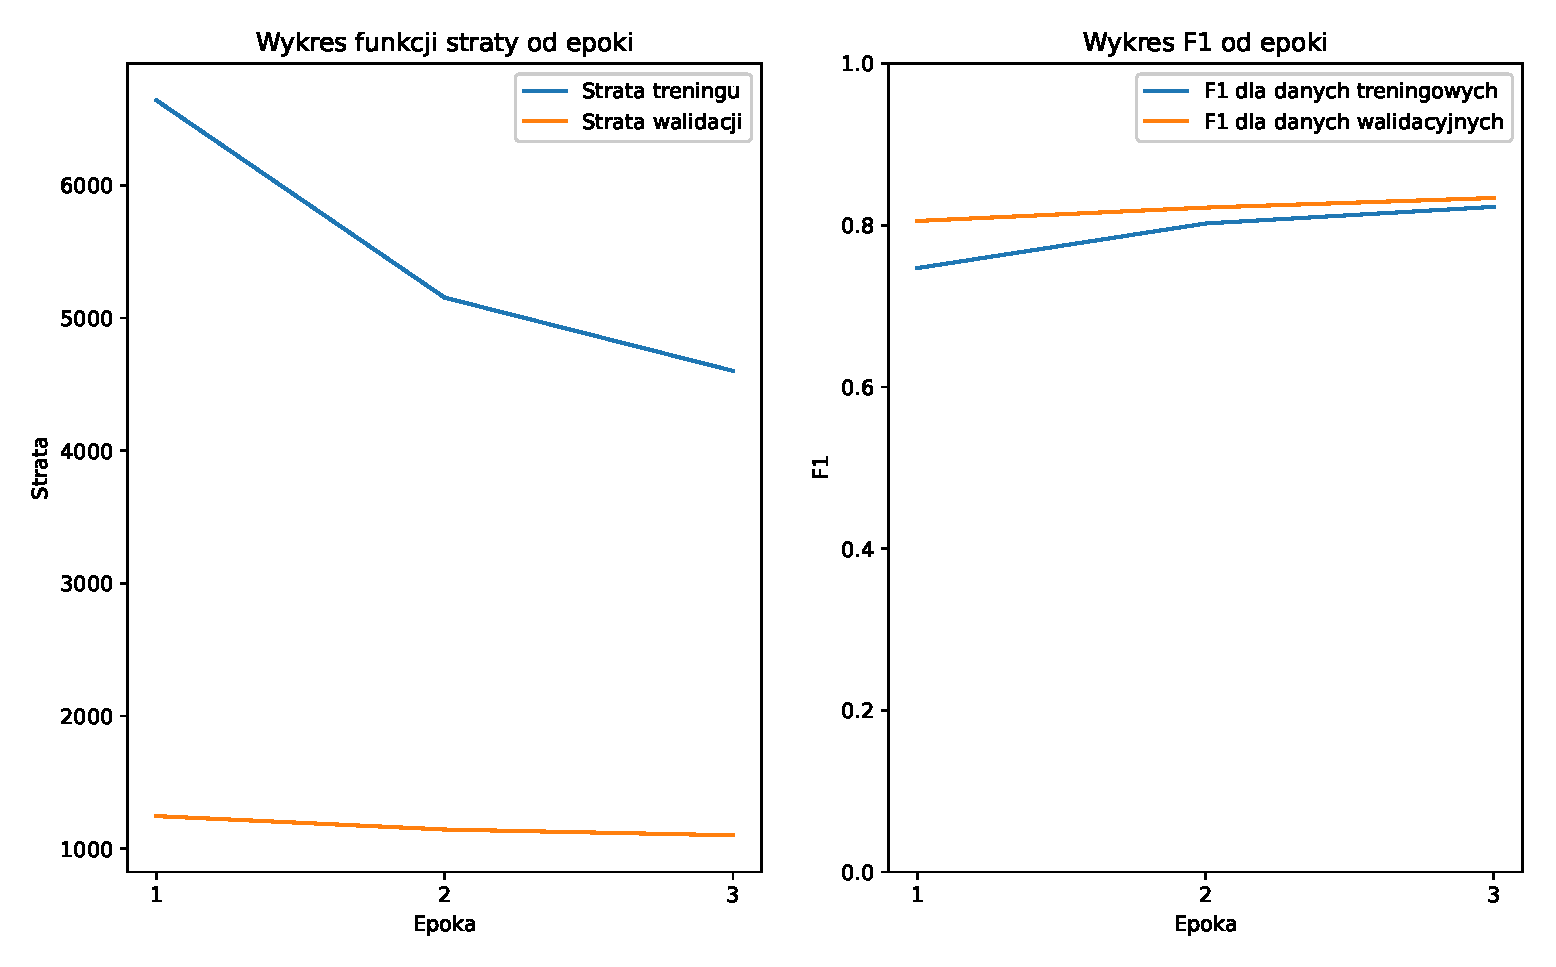
\includegraphics[width=\textwidth]{experiments/efficientnet_b0/combined}
    \caption{Wykres zależności funkcji straty i F1 od epoki trenowania (EfficientNet B0)}
    \label{fig:plot_efficientnet_b0}
\end{figure}
\begin{figure}
    \centering
    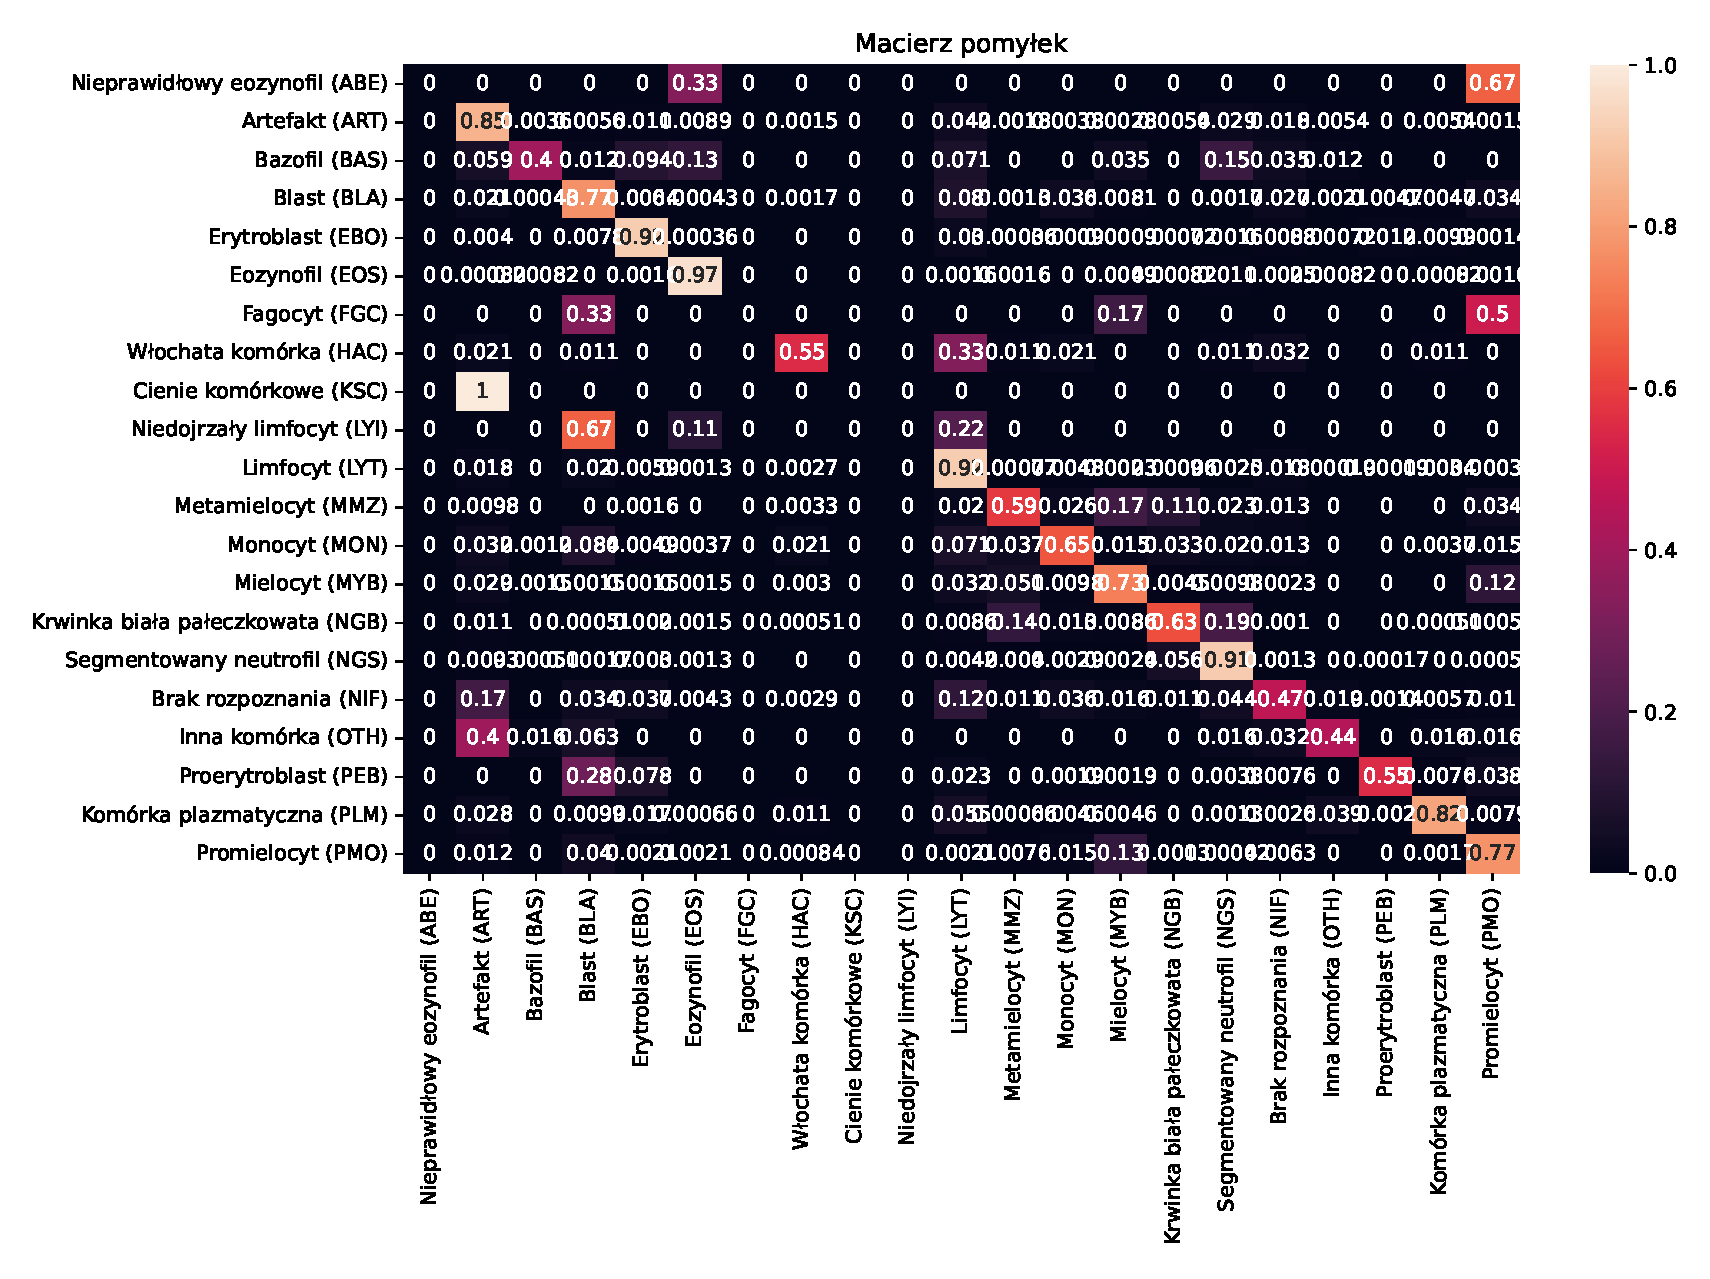
\includegraphics[width=0.8\textwidth]{experiments/efficientnet_b0/confusion_matrix}
    \caption{Macierz pomyłek modelu EfficientNet B0}
    \label{fig:confusion_efficientnet_b0}
\end{figure}

\begin{figure}
    \centering
    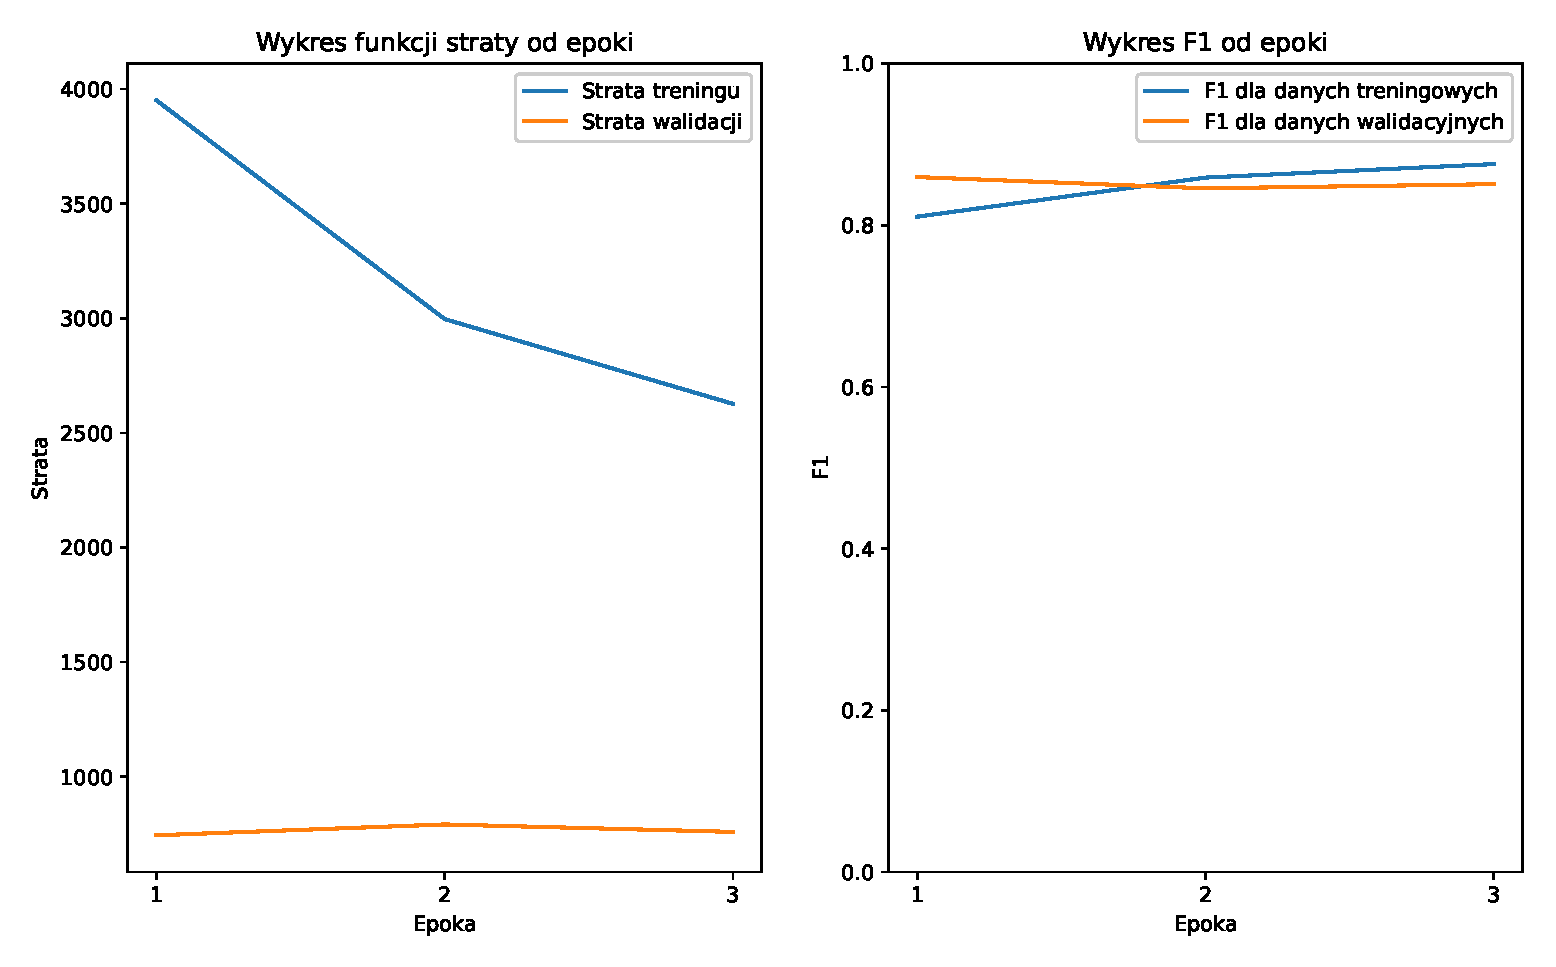
\includegraphics[width=\textwidth]{experiments/efficientnet_b1/combined}
    \caption{Wykres zależności funkcji straty i F1 od epoki trenowania (EfficientNet B1)}
    \label{fig:plot_efficientnet_b1}
\end{figure}
\begin{figure}
    \centering
    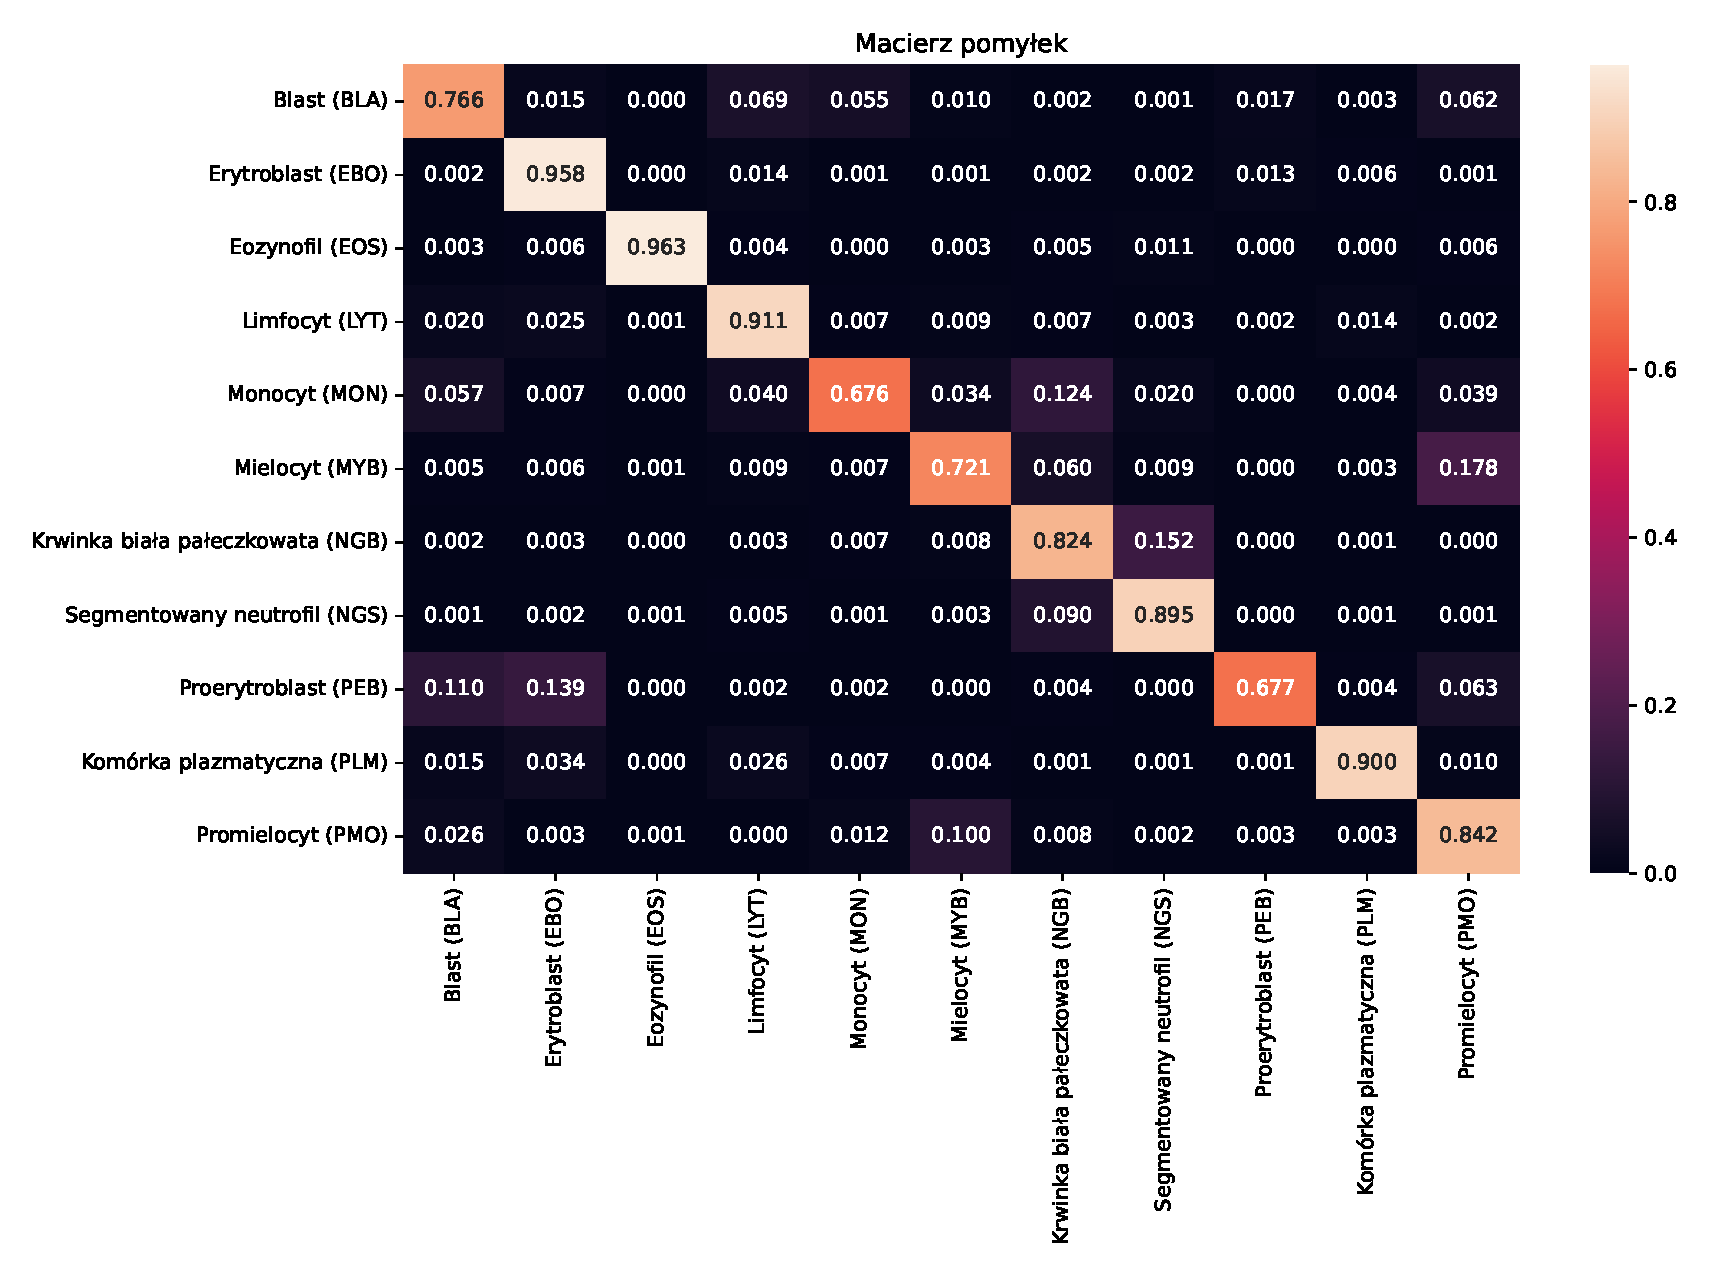
\includegraphics[width=0.8\textwidth]{experiments/efficientnet_b1/confusion_matrix}
    \caption{Macierz pomyłek modelu EfficientNet B1}
    \label{fig:confusion_efficientnet_b1}
\end{figure}

\begin{figure}
    \centering
    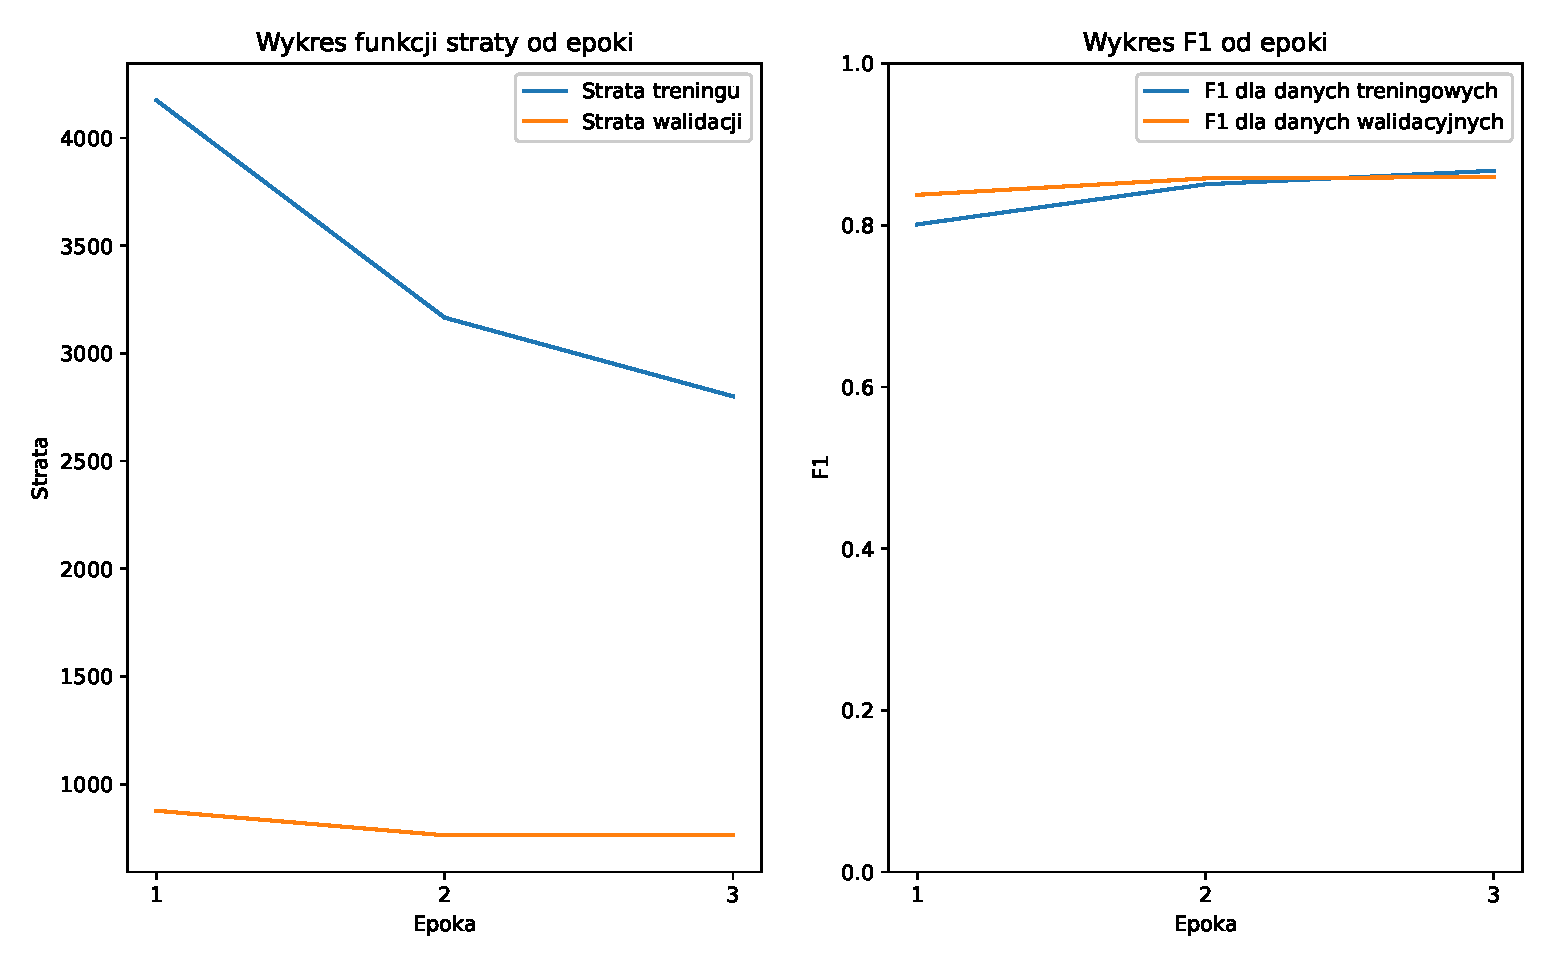
\includegraphics[width=\textwidth]{experiments/efficientnet_b2/combined}
    \caption{Wykres zależności funkcji straty i F1 od epoki trenowania (EfficientNet B2)}
    \label{fig:plot_efficientnet_b2}
\end{figure}
\begin{figure}
    \centering
    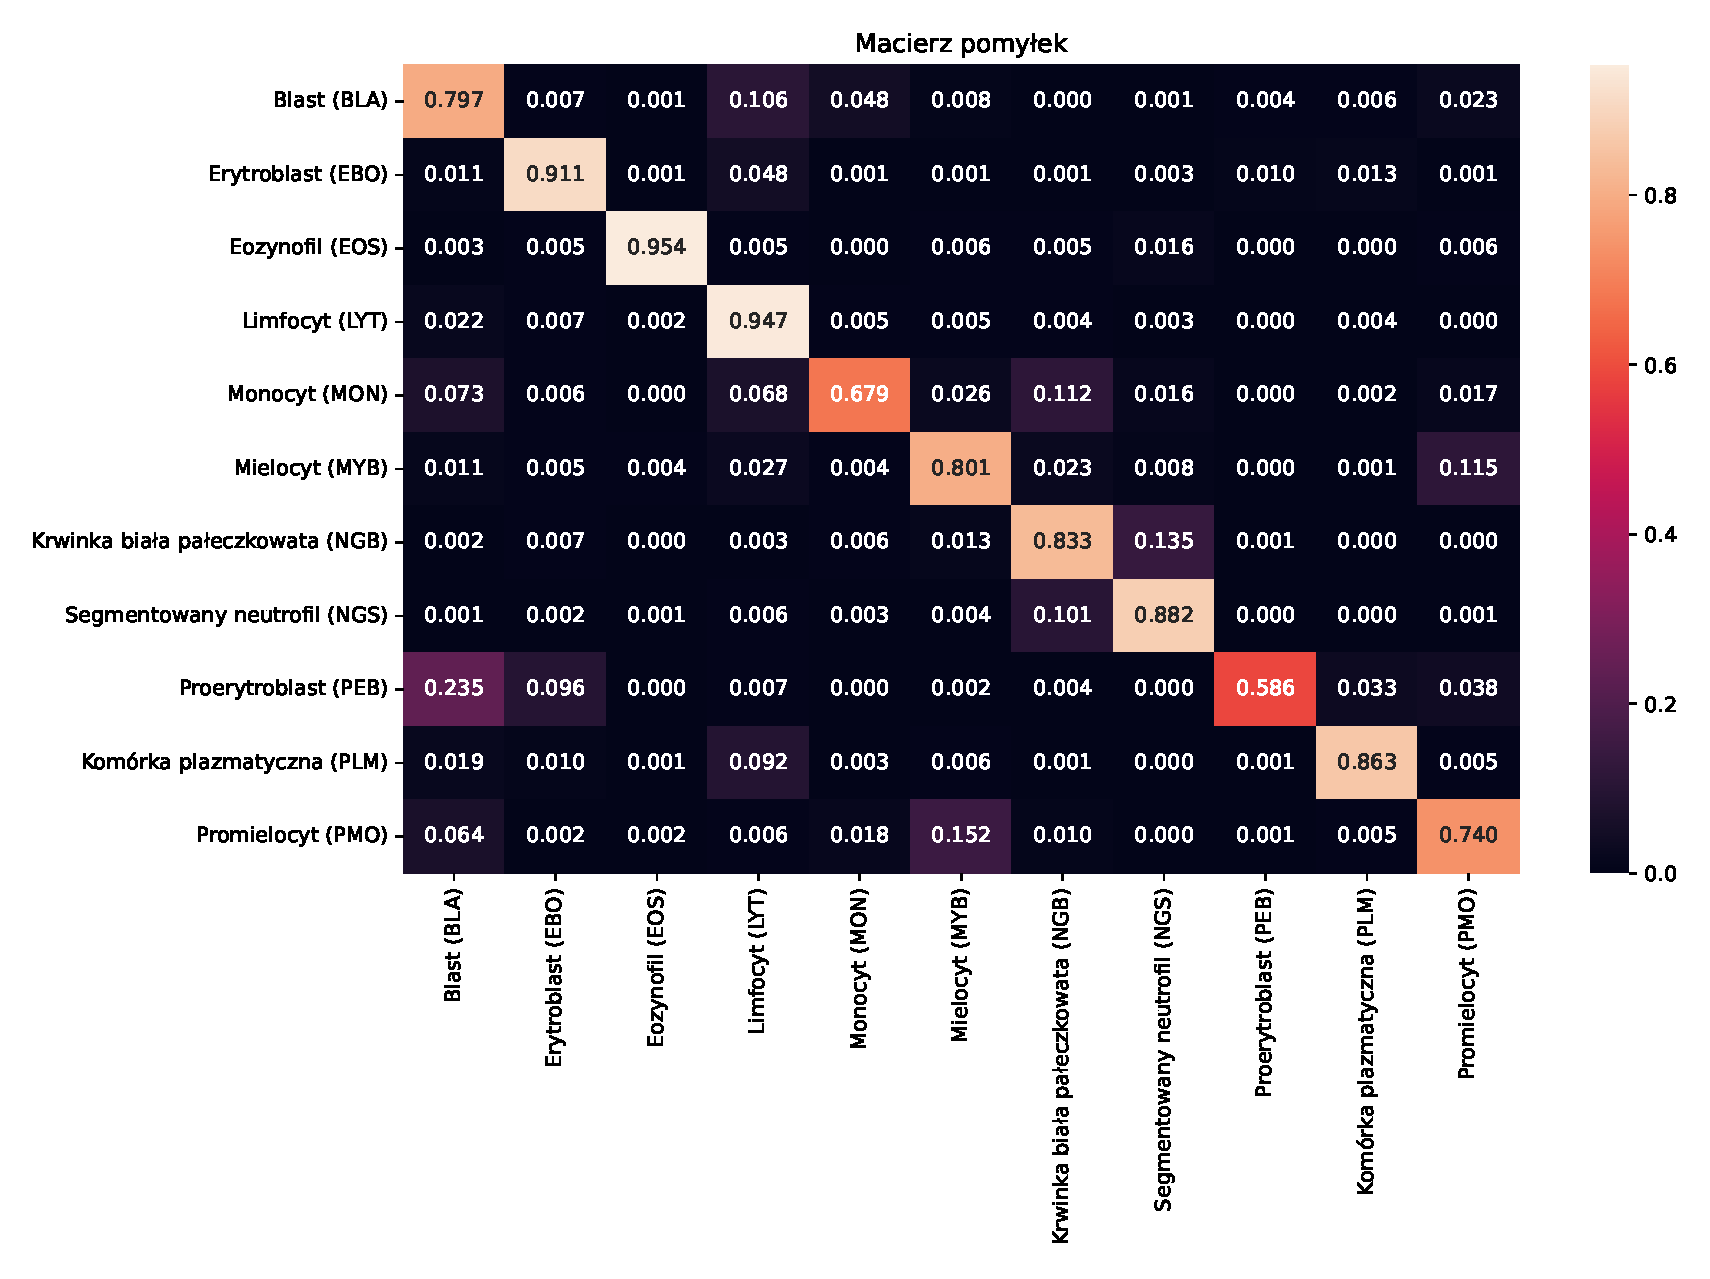
\includegraphics[width=0.8\textwidth]{experiments/efficientnet_b2/confusion_matrix}
    \caption{Macierz pomyłek modelu EfficientNet B2}
    \label{fig:confusion_efficientnet_b2}
\end{figure}

\begin{figure}
    \centering
    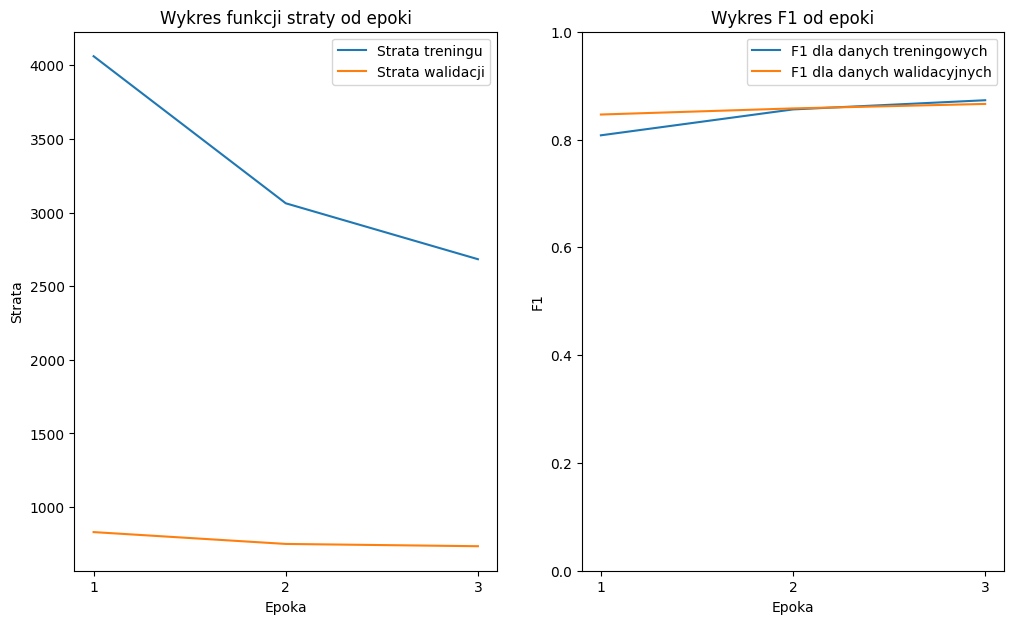
\includegraphics[width=\textwidth]{experiments/efficientnet_b3/combined}
    \caption{Wykres zależności funkcji straty i F1 od epoki trenowania (EfficientNet B3)}
    \label{fig:plot_efficientnet_b3}
\end{figure}
\begin{figure}
    \centering
    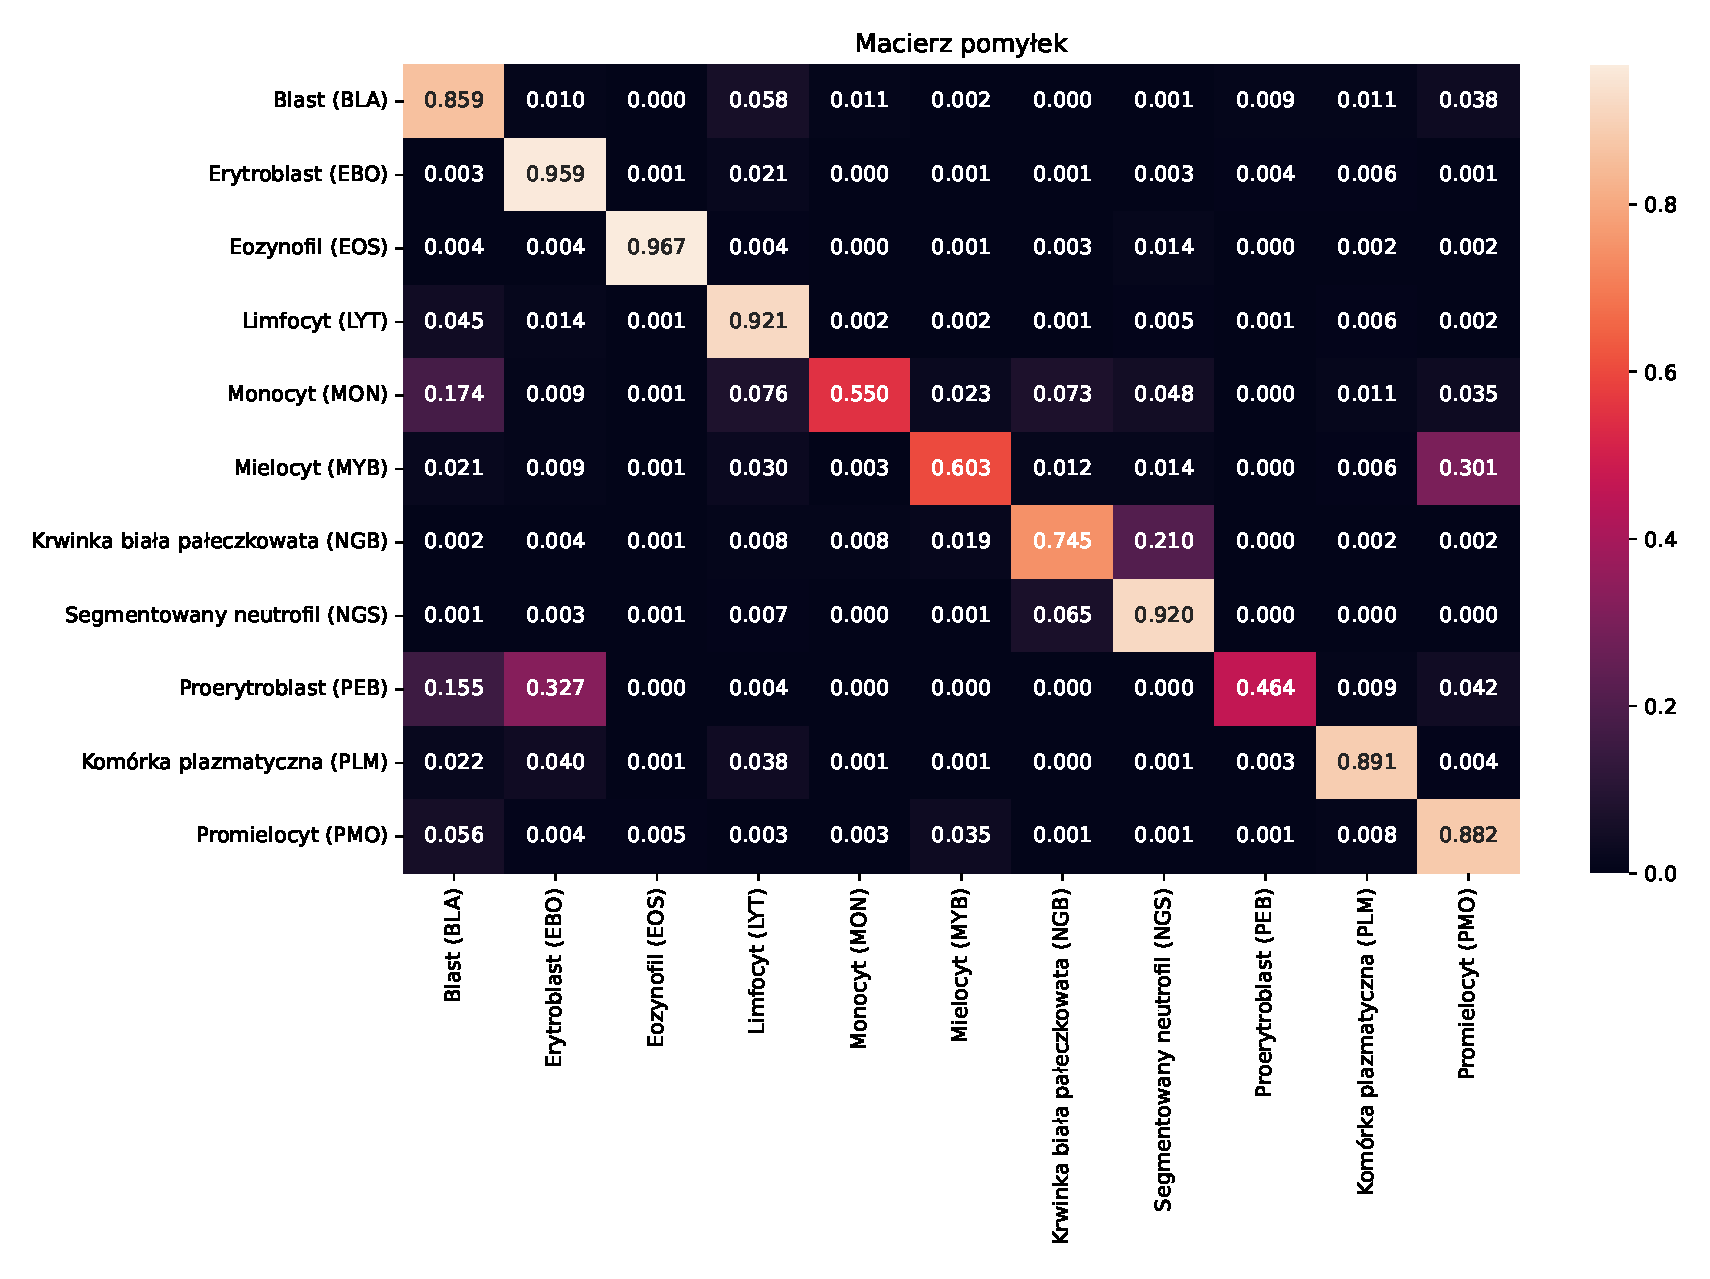
\includegraphics[width=0.8\textwidth]{experiments/efficientnet_b3/confusion_matrix}
    \caption{Macierz pomyłek modelu EfficientNet B3}
    \label{fig:confusion_efficientnet_b3}
\end{figure}

\begin{figure}
    \centering
    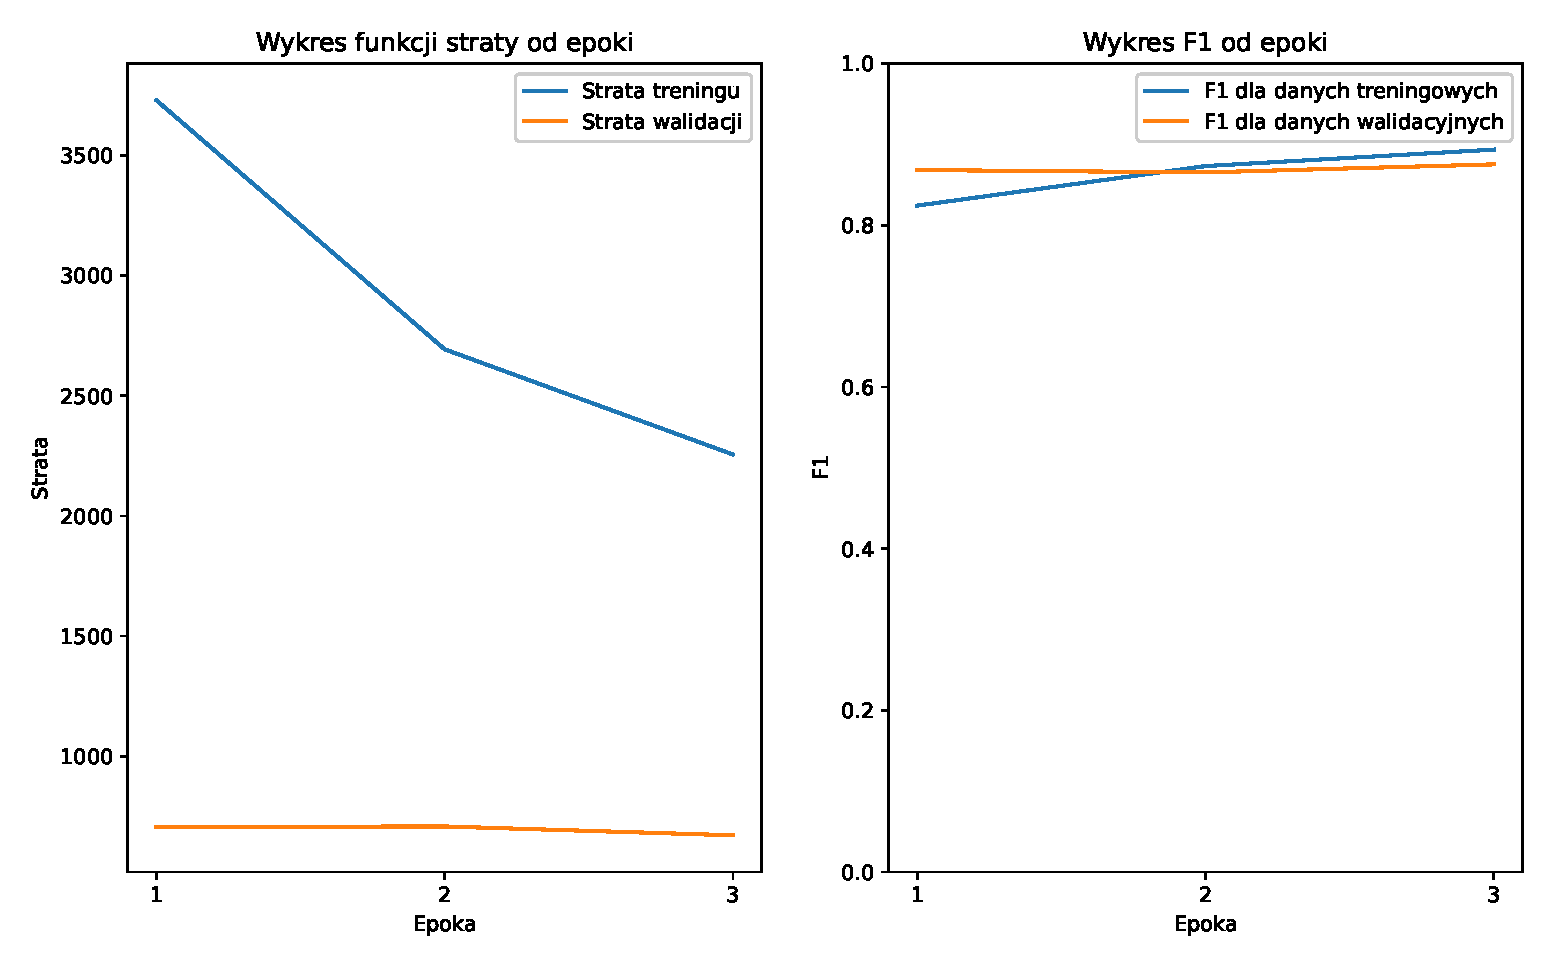
\includegraphics[width=\textwidth]{experiments/efficientnet_b4/combined}
    \caption{Wykres zależności funkcji straty i F1 od epoki trenowania (EfficientNet B4)}
    \label{fig:plot_efficientnet_b4}
\end{figure}
\begin{figure}
    \centering
    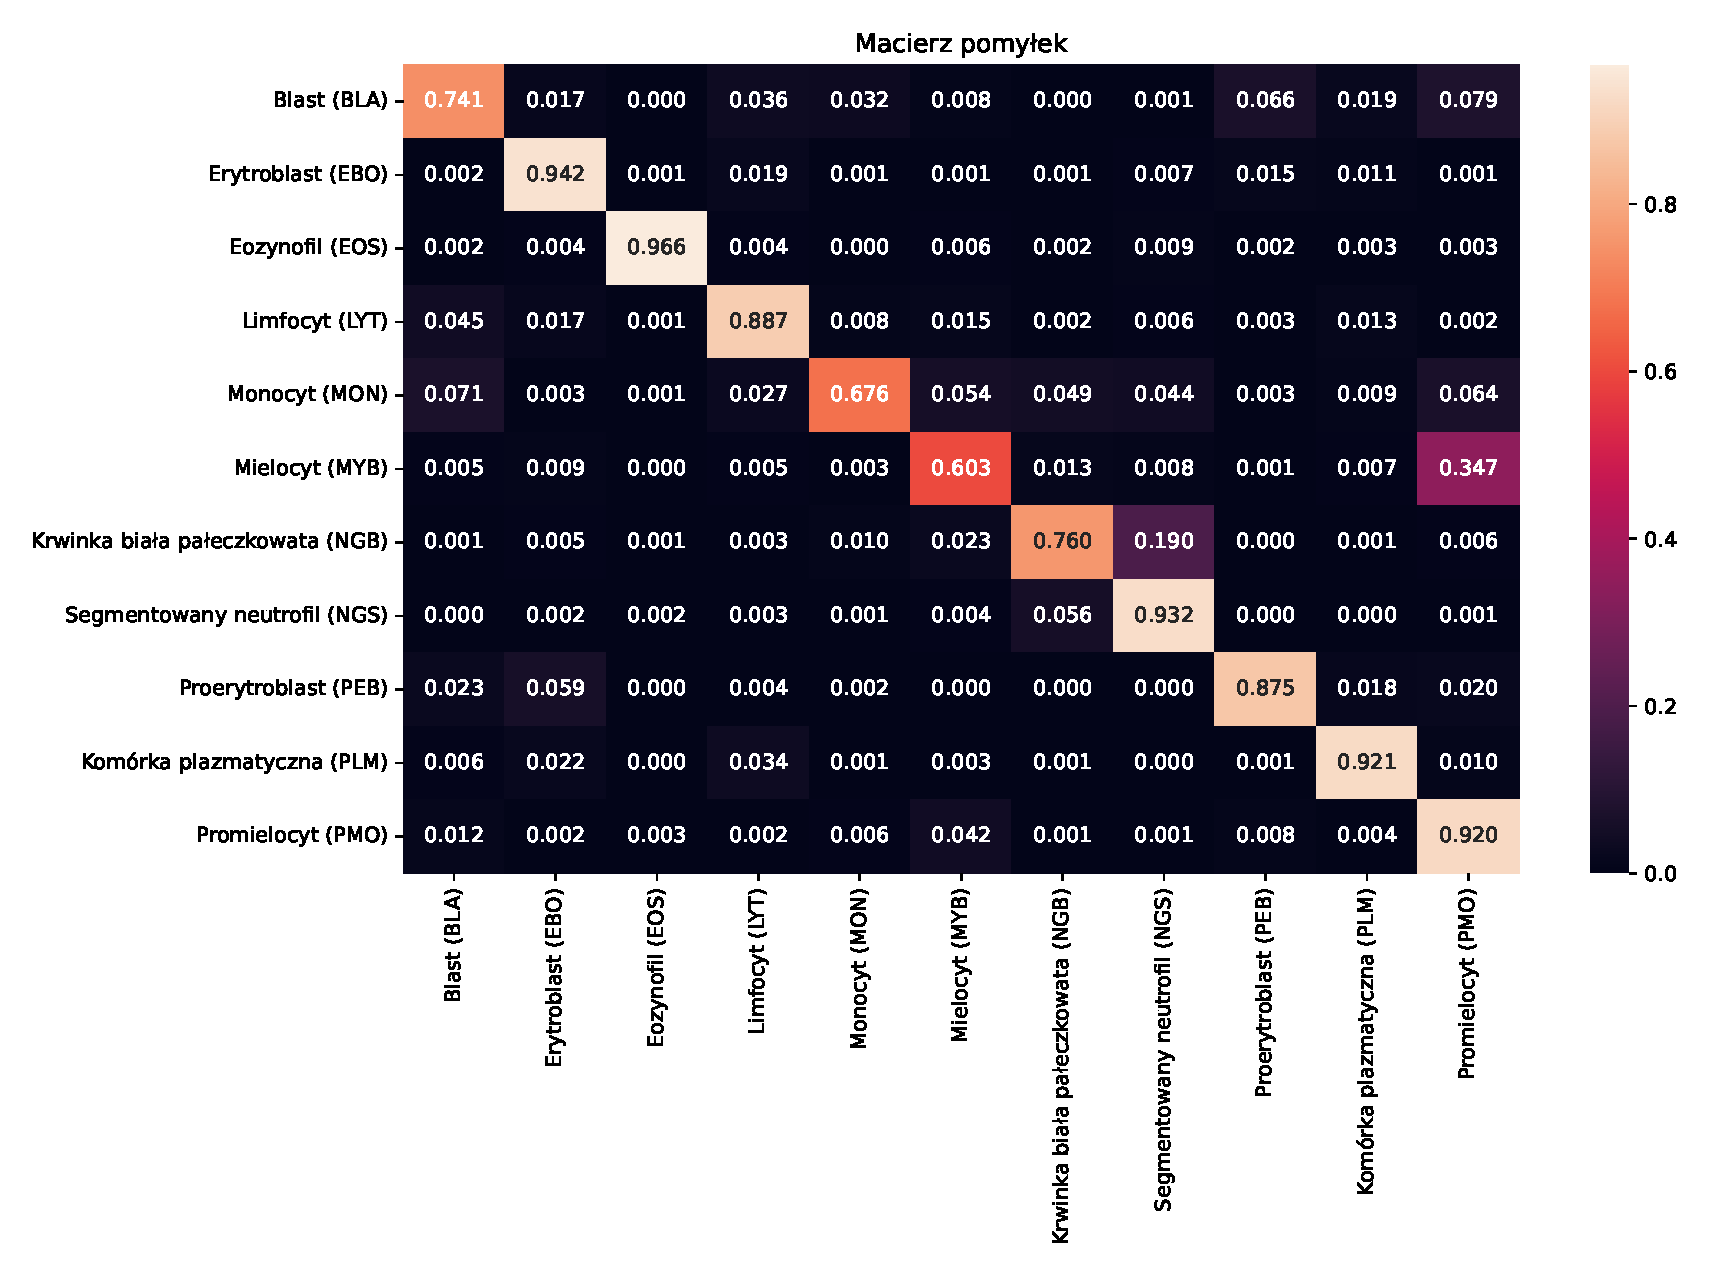
\includegraphics[width=0.8\textwidth]{experiments/efficientnet_b4/confusion_matrix}
    \caption{Macierz pomyłek modelu EfficientNet B4}
    \label{fig:confusion_efficientnet_b4}
\end{figure}

\begin{figure}
    \centering
    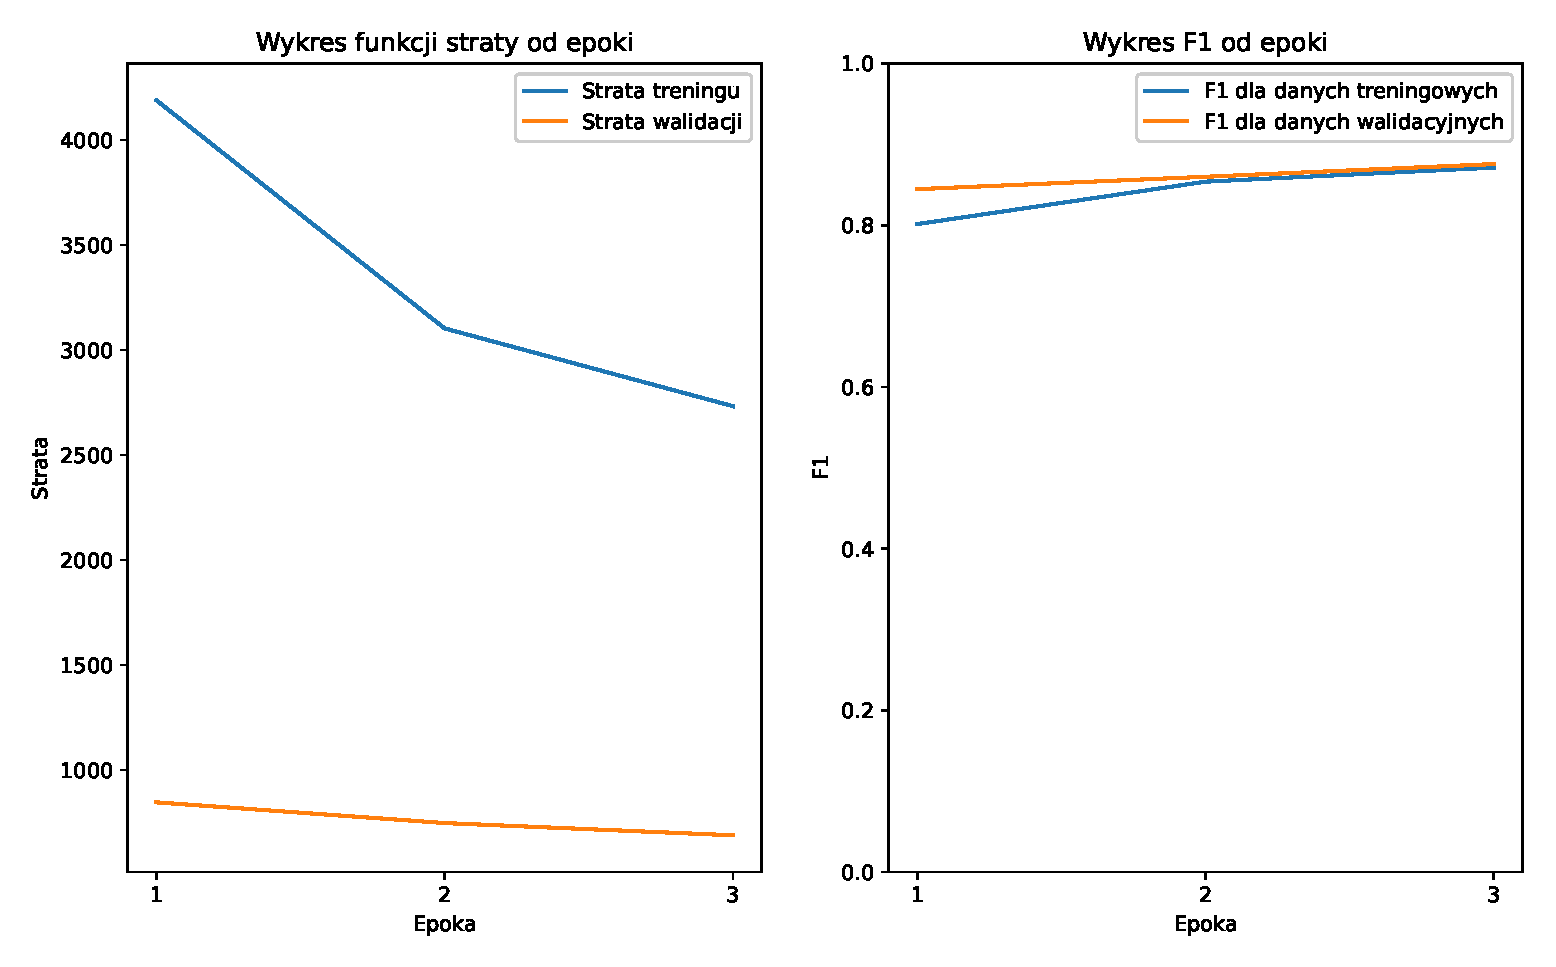
\includegraphics[width=\textwidth]{experiments/efficientnet_b5/combined}
    \caption{Wykres zależności funkcji straty i F1 od epoki trenowania (EfficientNet B5)}
    \label{fig:plot_efficientnet_b5}
\end{figure}
\begin{figure}
    \centering
    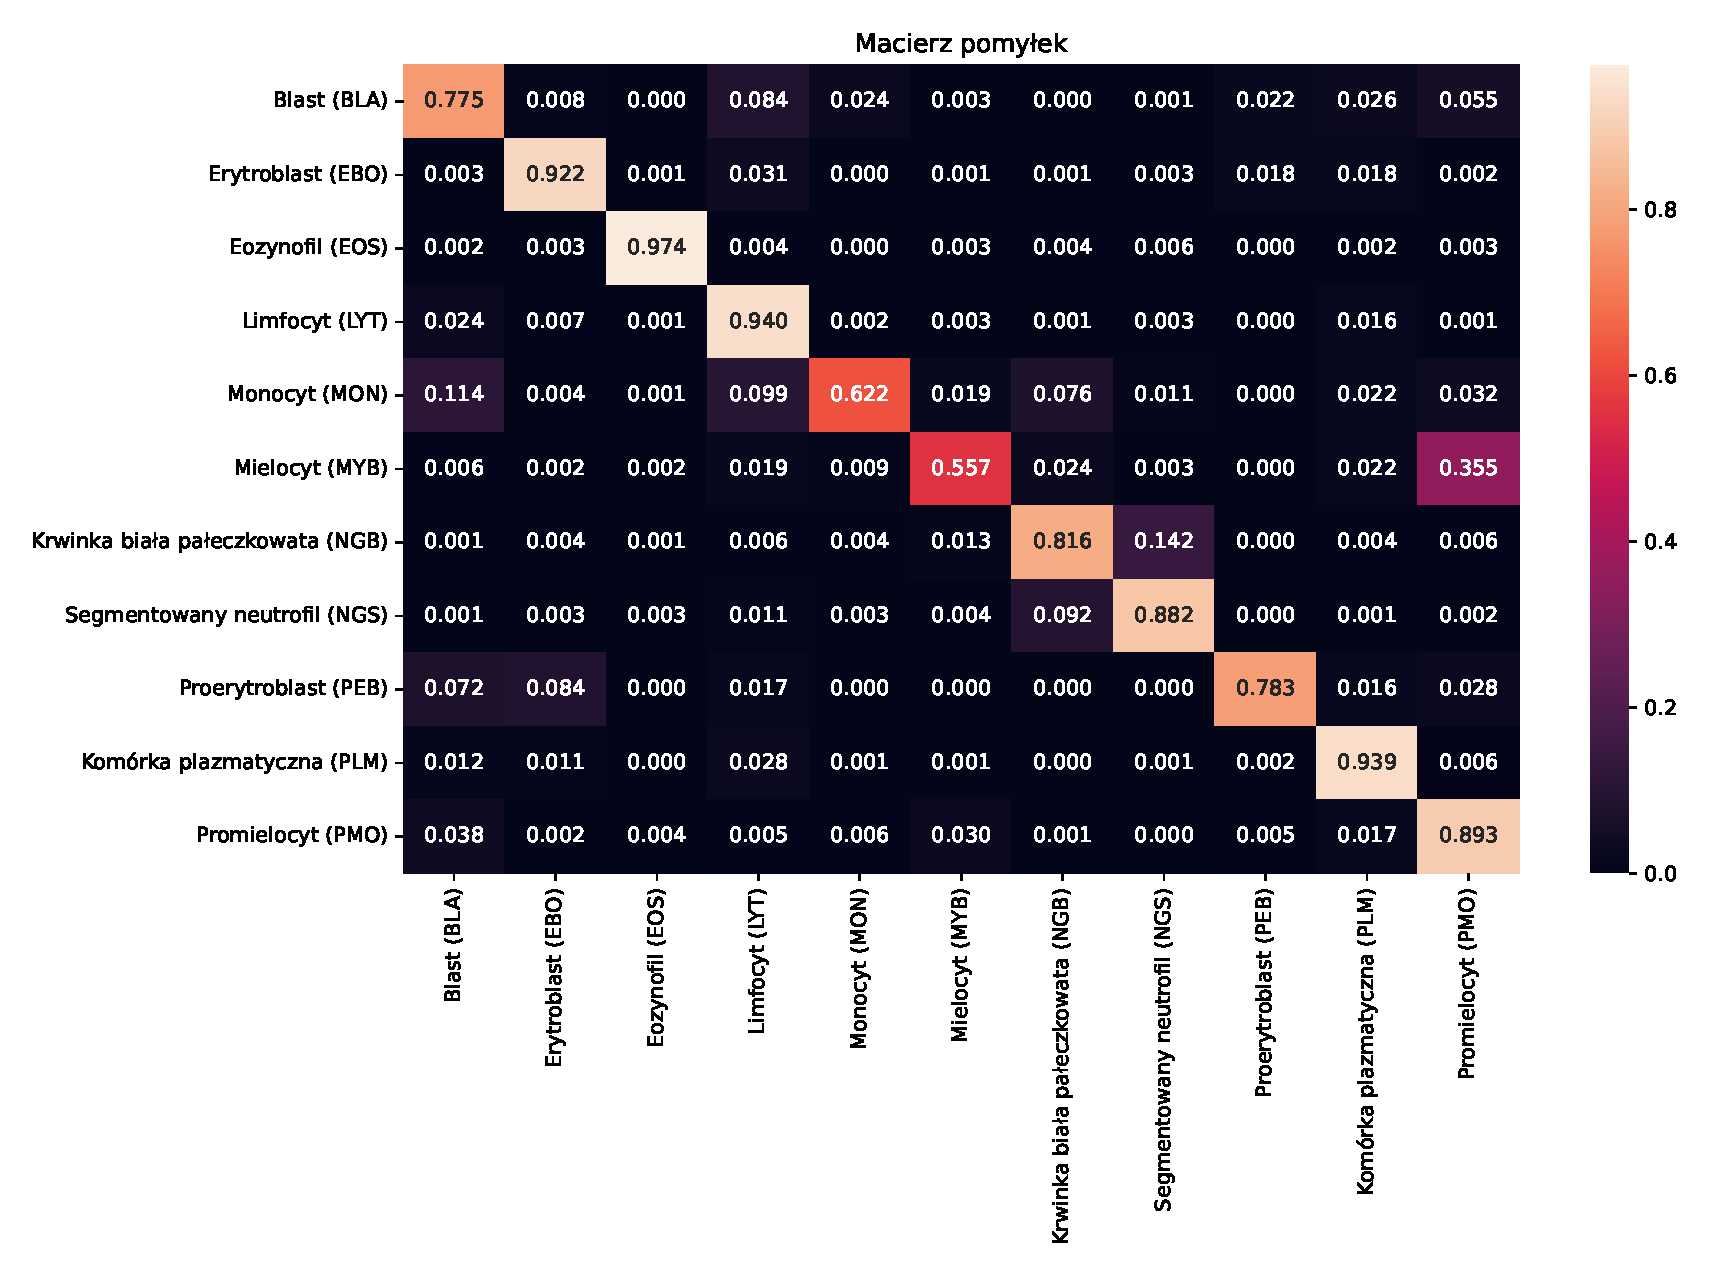
\includegraphics[width=0.8\textwidth]{experiments/efficientnet_b5/confusion_matrix}
    \caption{Macierz pomyłek modelu EfficientNet B5}
    \label{fig:confusion_efficientnet_b5}
\end{figure}

\begin{figure}
    \centering
    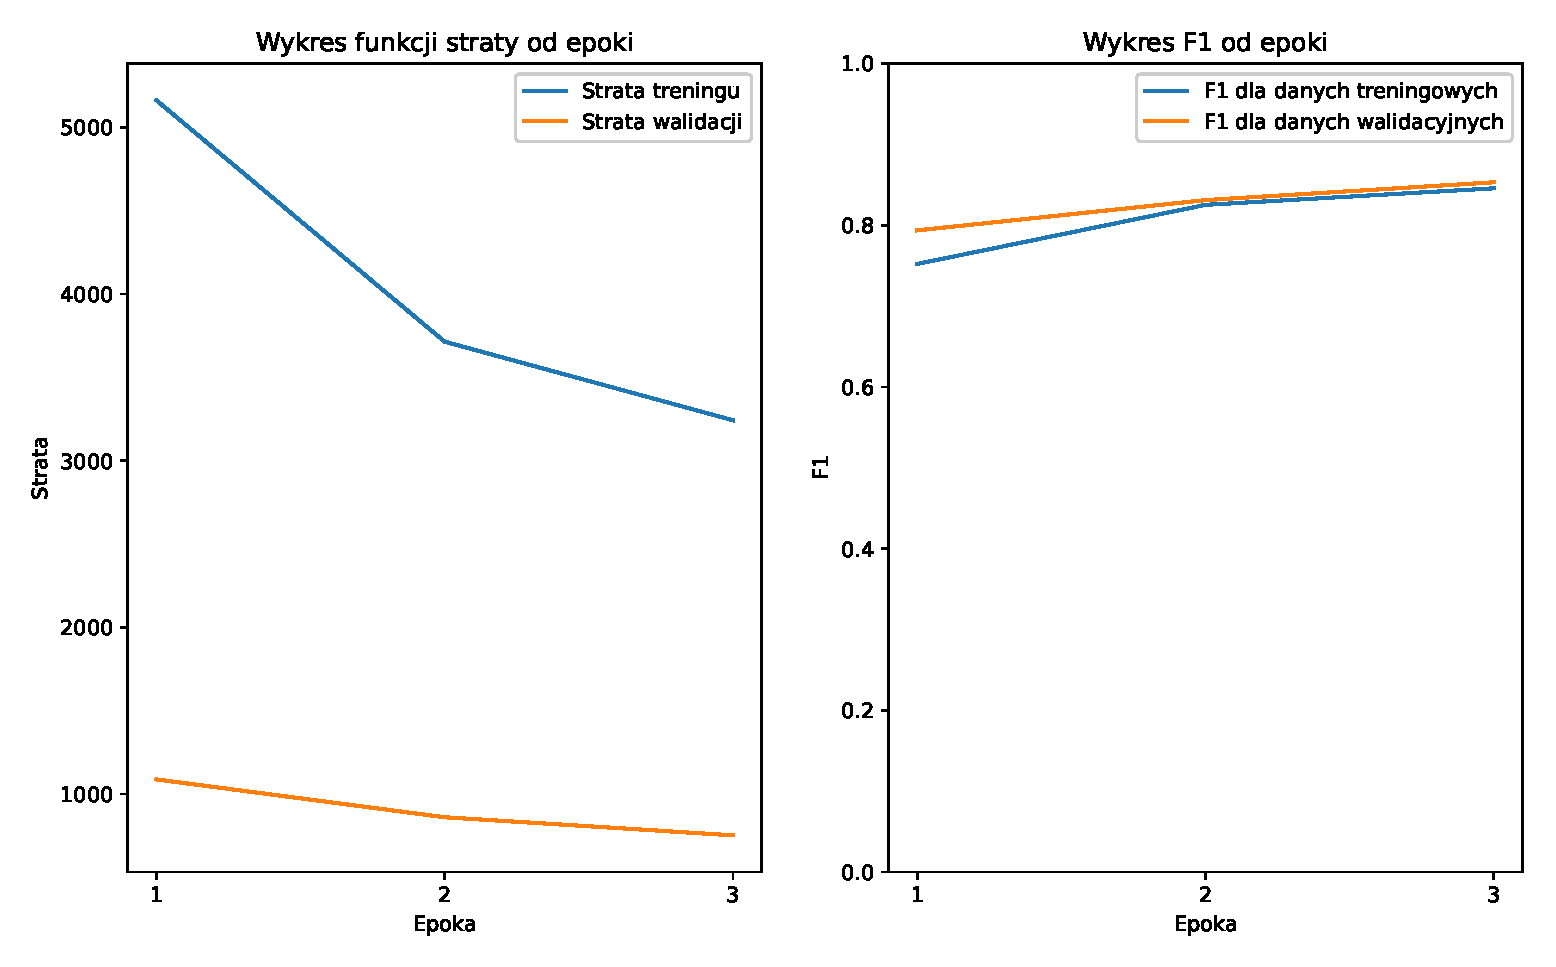
\includegraphics[width=\textwidth]{experiments/densenet121/combined}
    \caption{Wykres zależności funkcji straty i F1 od epoki trenowania (DenseNet121)}
    \label{fig:plot_densenet121}
\end{figure}
\begin{figure}
    \centering
    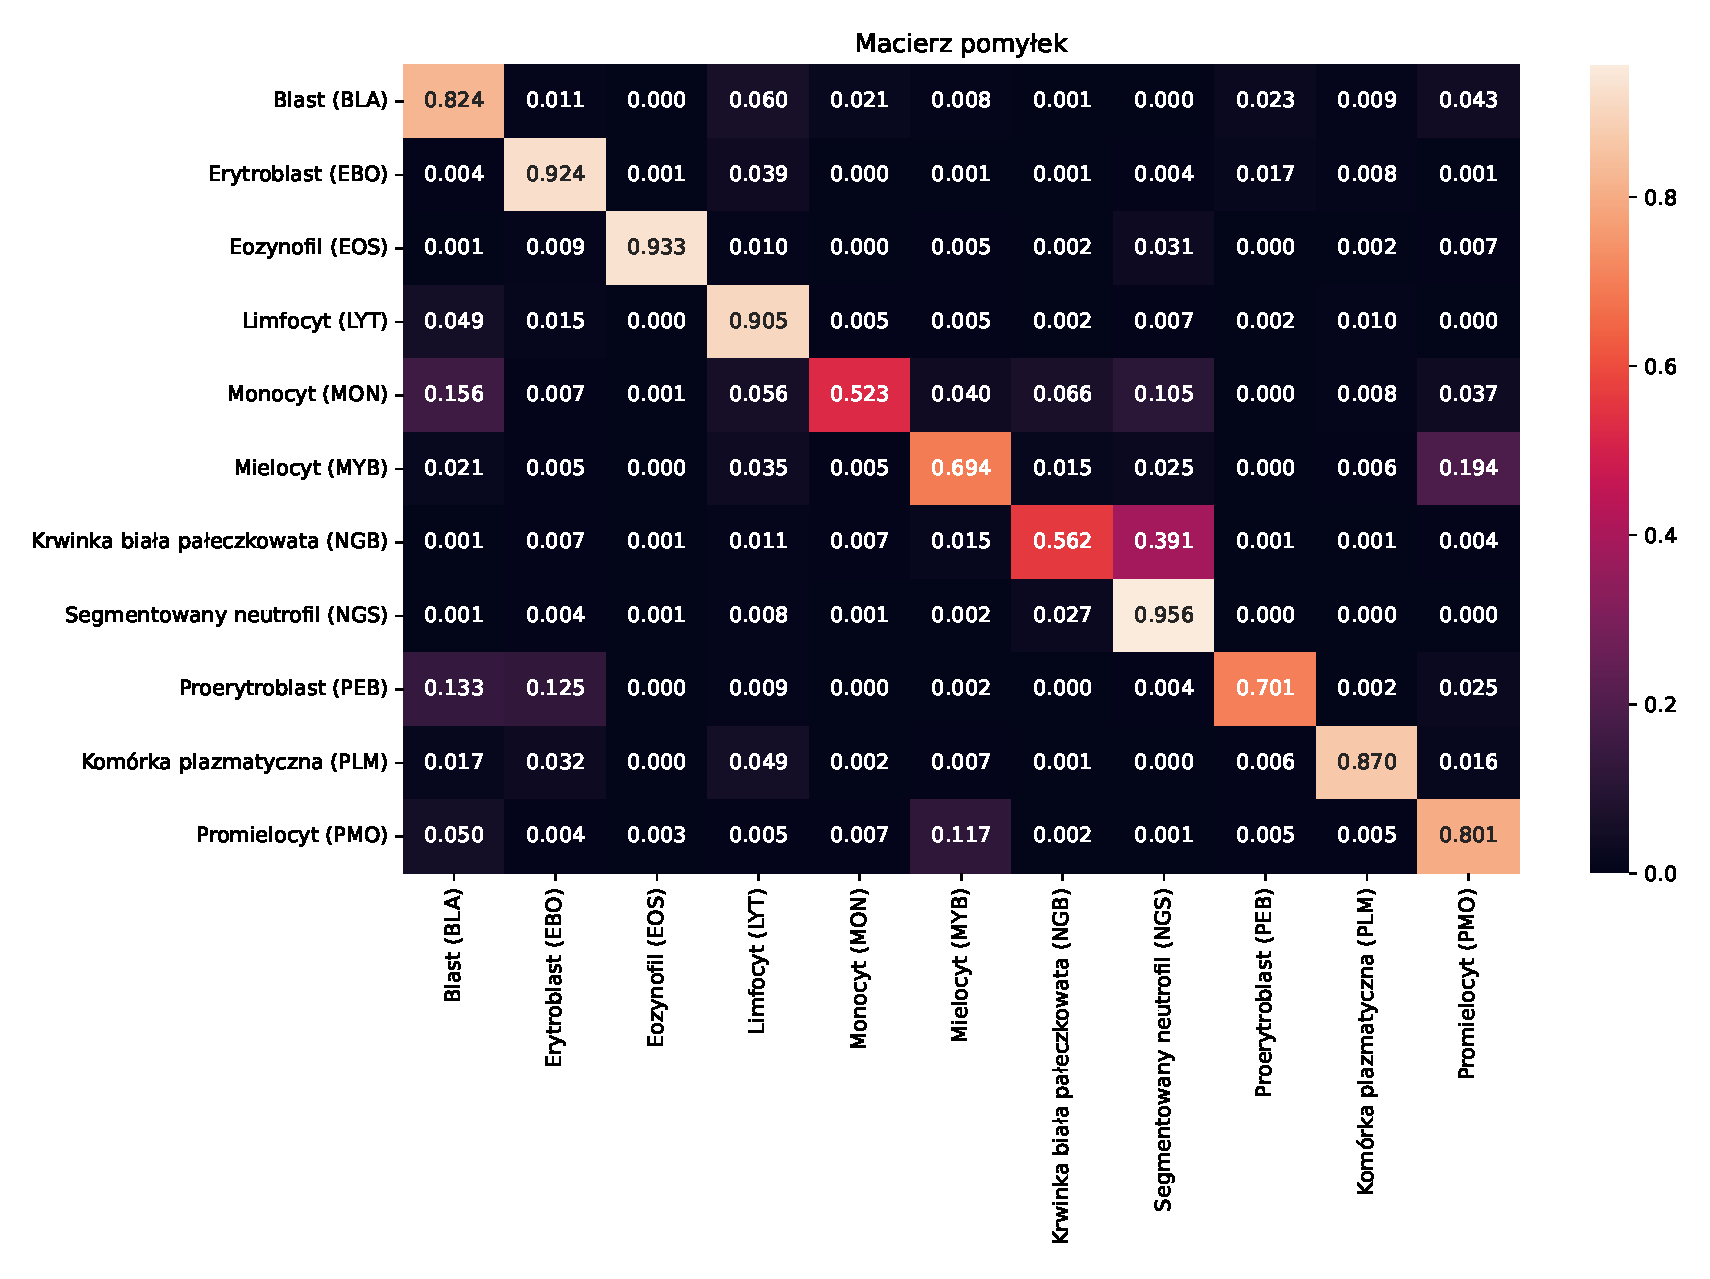
\includegraphics[width=0.8\textwidth]{experiments/densenet121/confusion_matrix}
    \caption{Macierz pomyłek modelu DenseNet121}
    \label{fig:confusion_densenet121}
\end{figure}

\begin{figure}
    \centering
    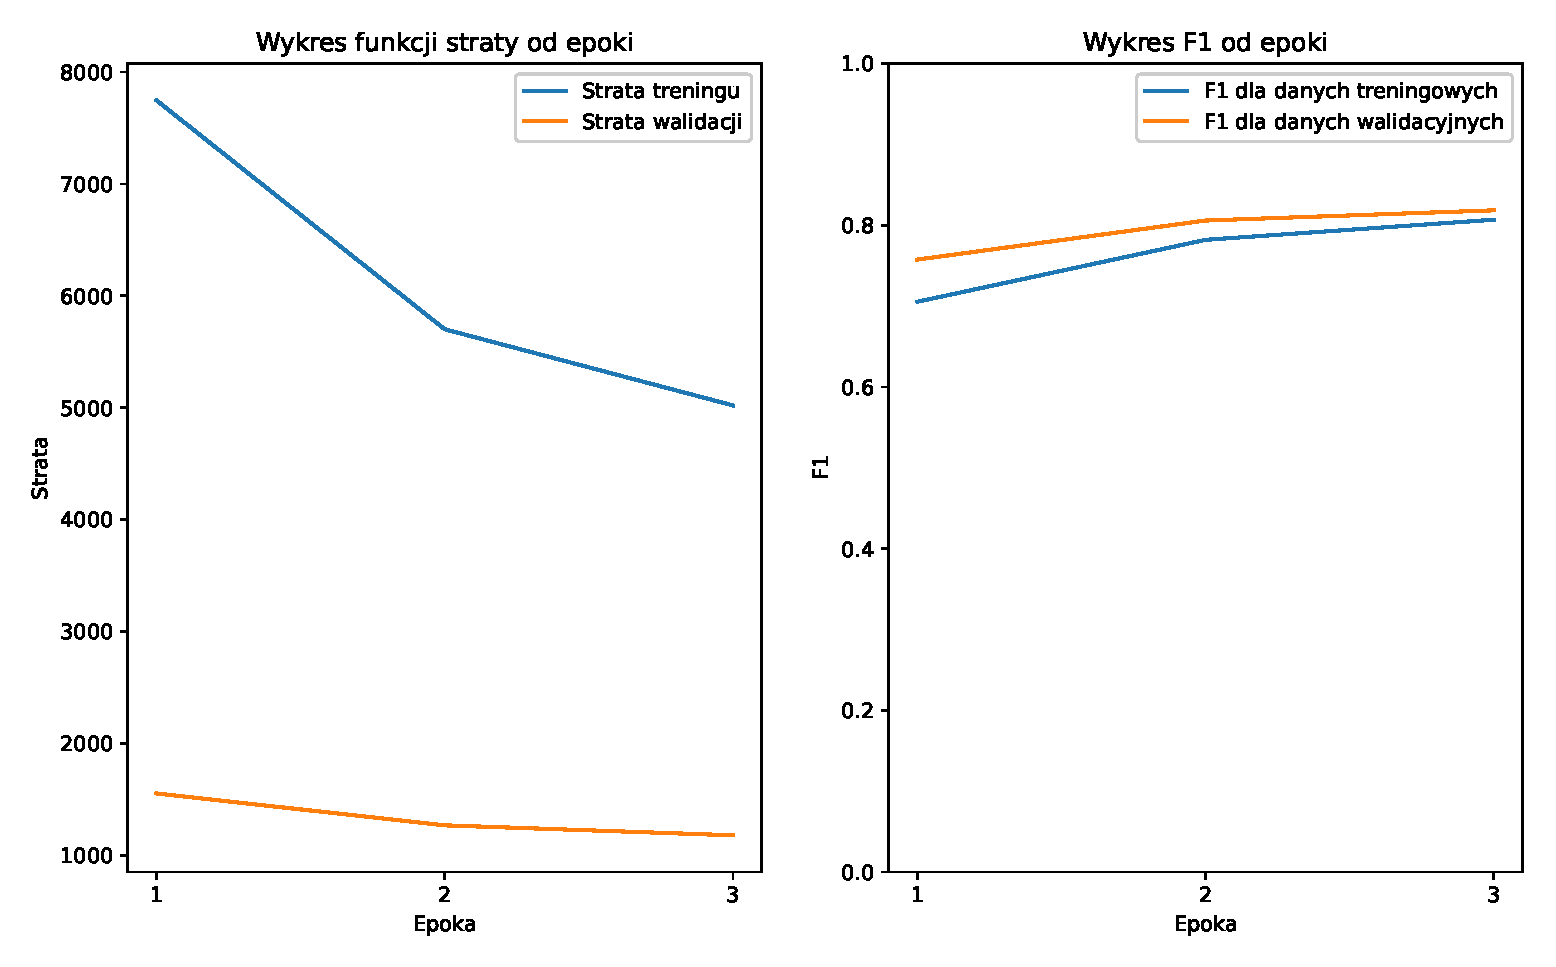
\includegraphics[width=\textwidth]{experiments/densenet169/combined}
    \caption{Wykres zależności funkcji straty i F1 od epoki trenowania (DenseNet169)}
    \label{fig:plot_densenet169}
\end{figure}
\begin{figure}
    \centering
    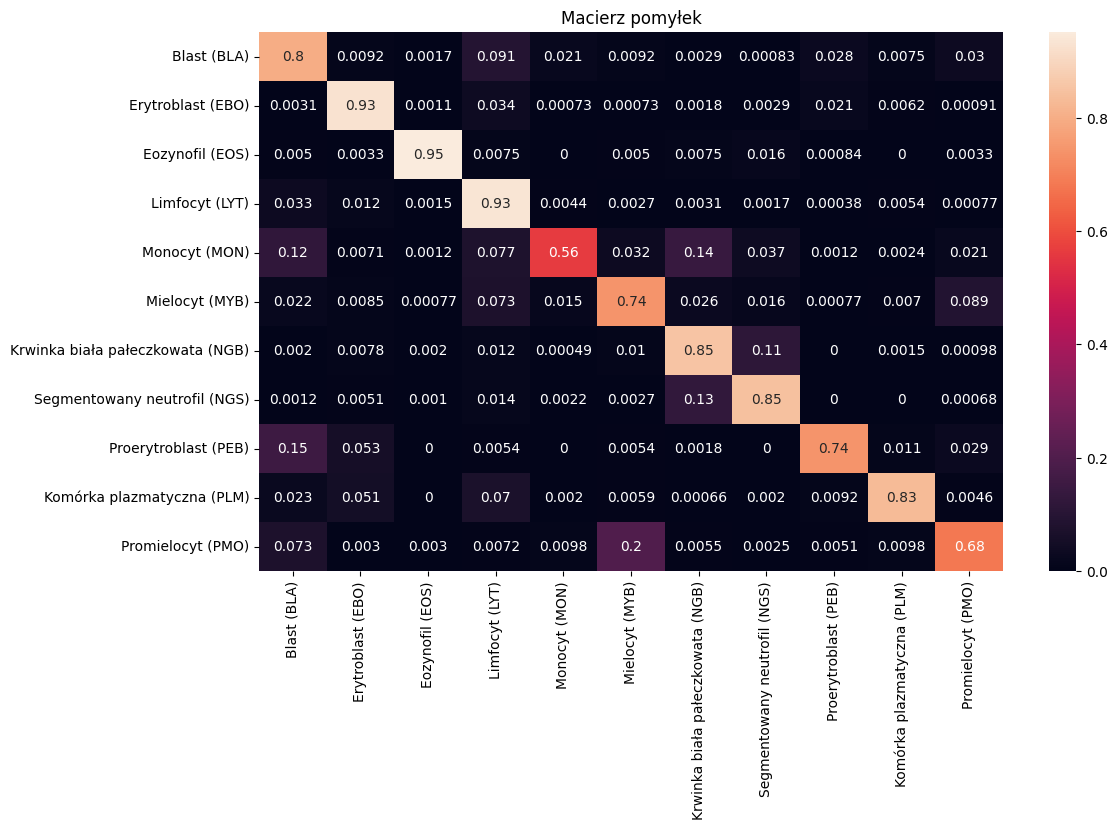
\includegraphics[width=0.8\textwidth]{experiments/densenet169/confusion_matrix}
    \caption{Macierz pomyłek modelu DenseNet169}
    \label{fig:confusion_densenet169}
\end{figure}

\begin{figure}
    \centering
    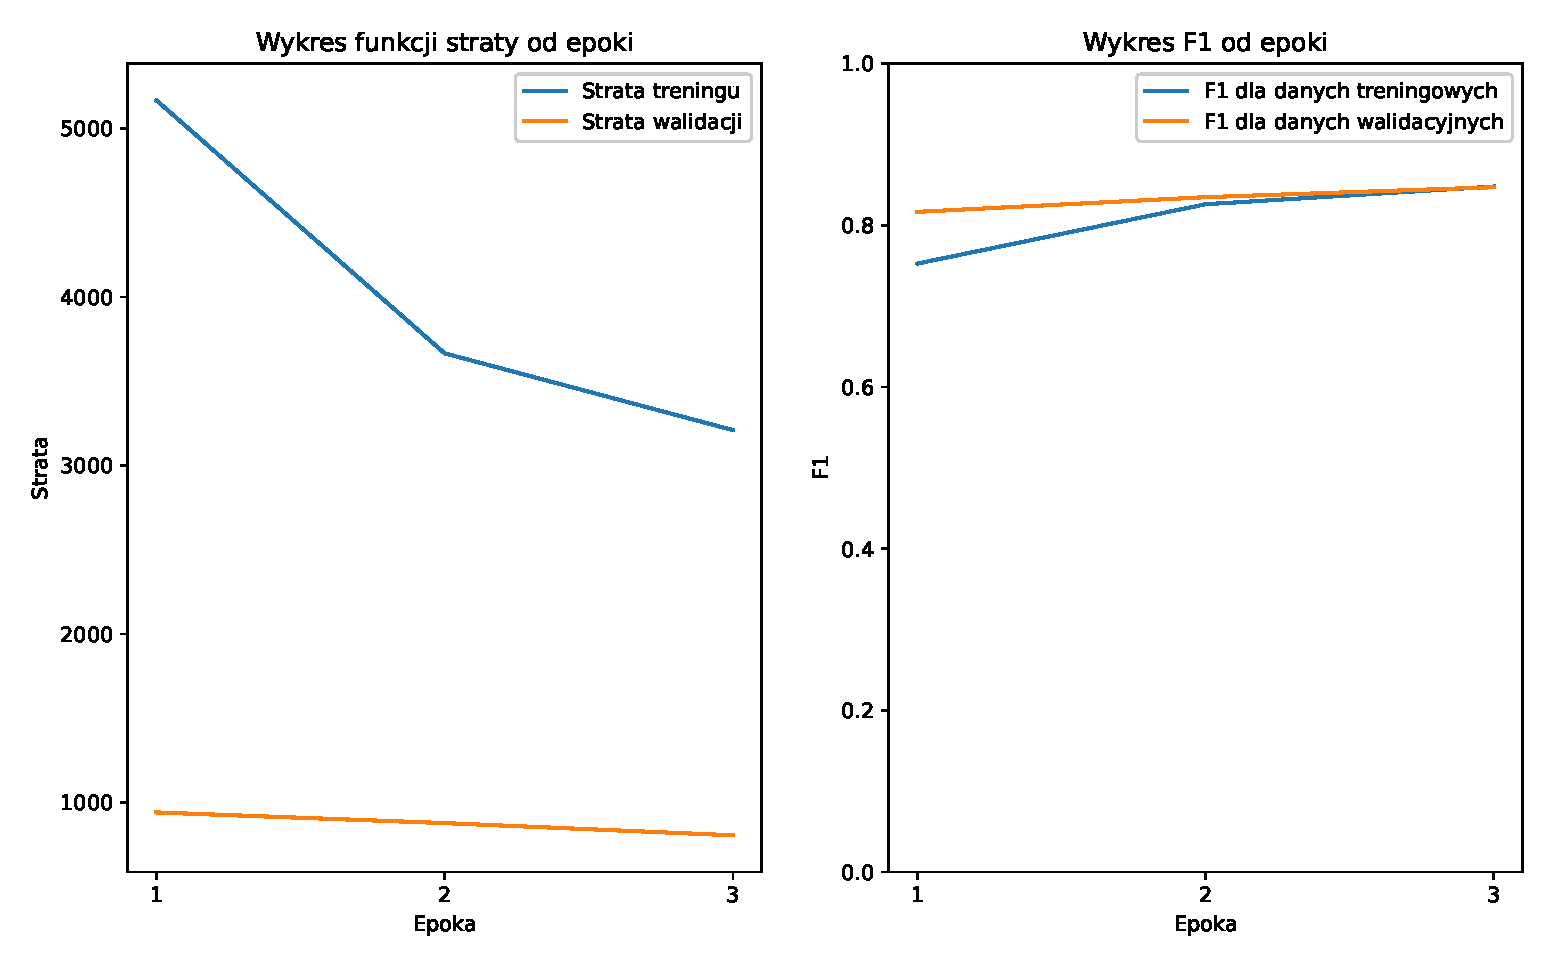
\includegraphics[width=\textwidth]{experiments/densenet201/combined}
    \caption{Wykres zależności funkcji straty i F1 od epoki trenowania (DenseNet201)}
    \label{fig:plot_densenet201}
\end{figure}
\begin{figure}
    \centering
    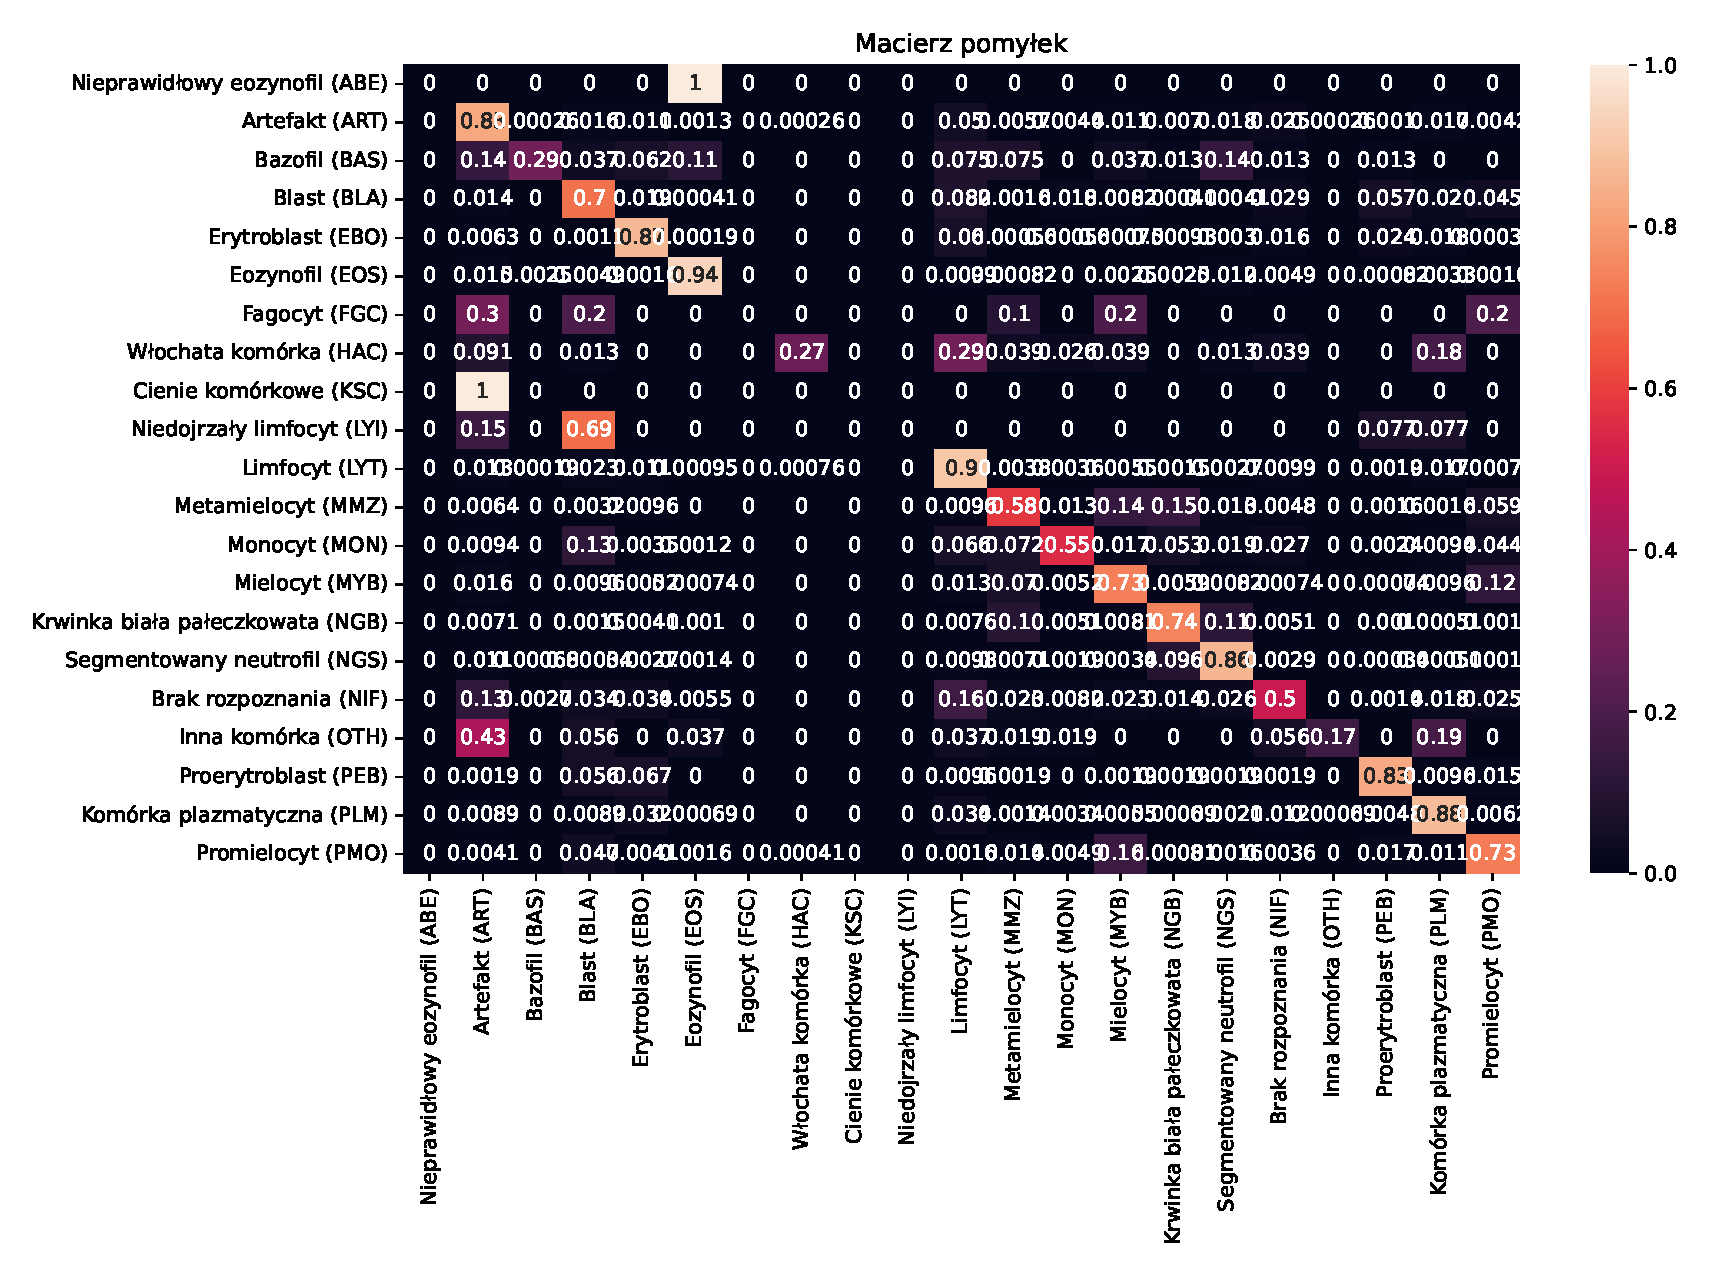
\includegraphics[width=0.8\textwidth]{experiments/densenet201/confusion_matrix}
    \caption{Macierz pomyłek modelu DenseNet201}
    \label{fig:confusion_densenet201}
\end{figure}

\begin{figure}
    \centering
    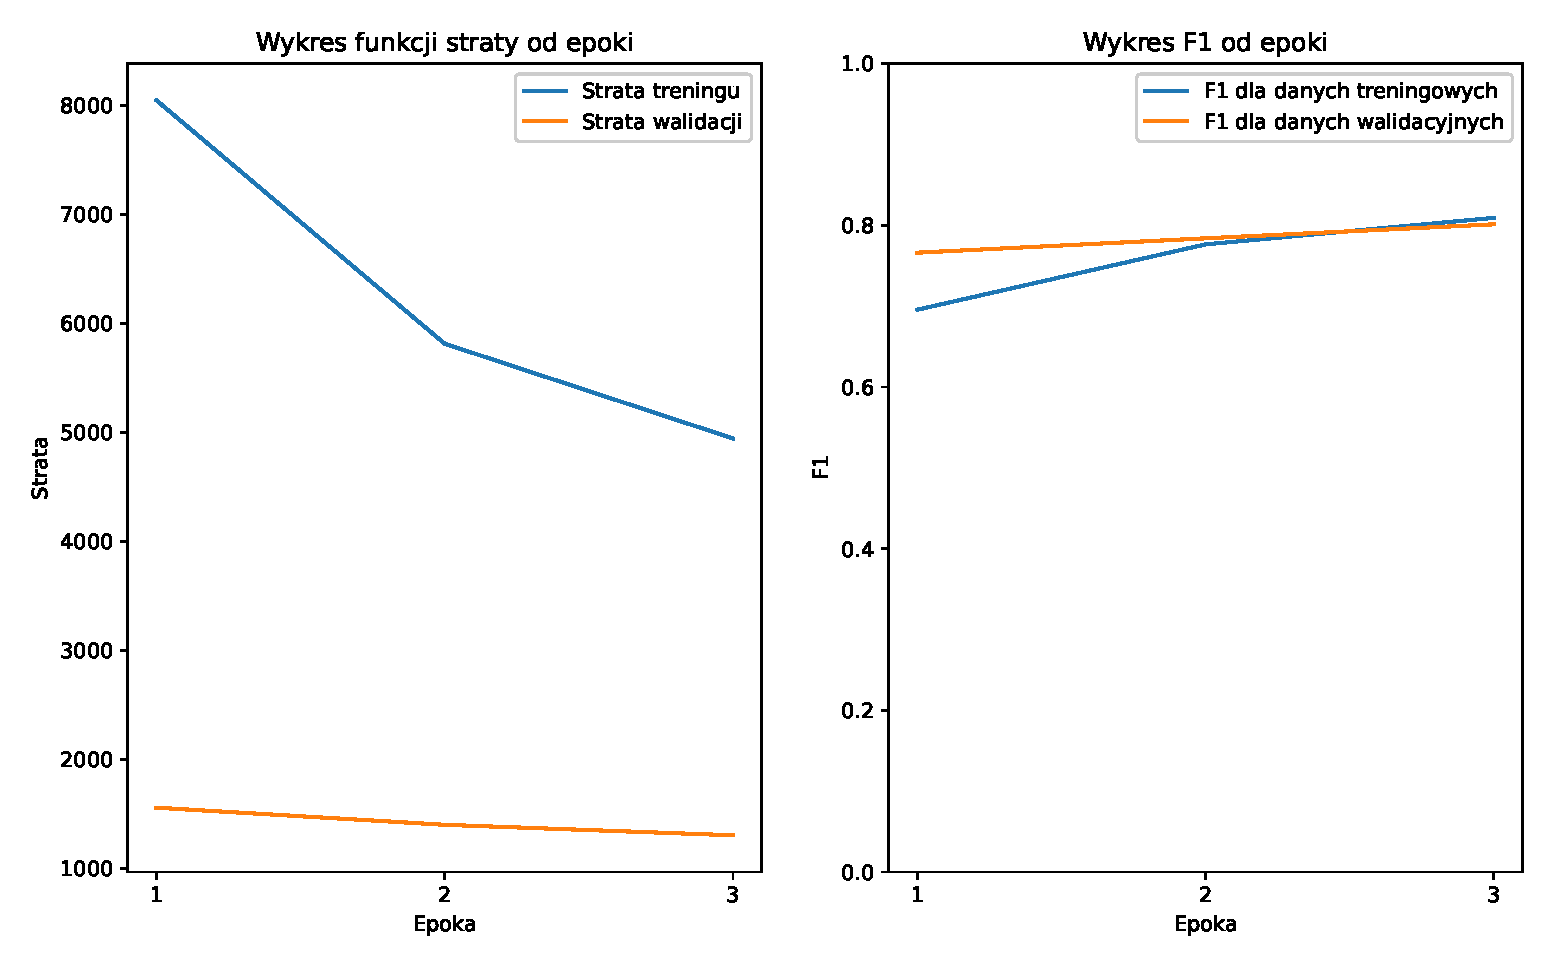
\includegraphics[width=\textwidth]{experiments/resnet18/combined}
    \caption{Wykres zależności funkcji straty i F1 od epoki trenowania (ResNet18)}
    \label{fig:plot_resnet18}
\end{figure}
\begin{figure}
    \centering
    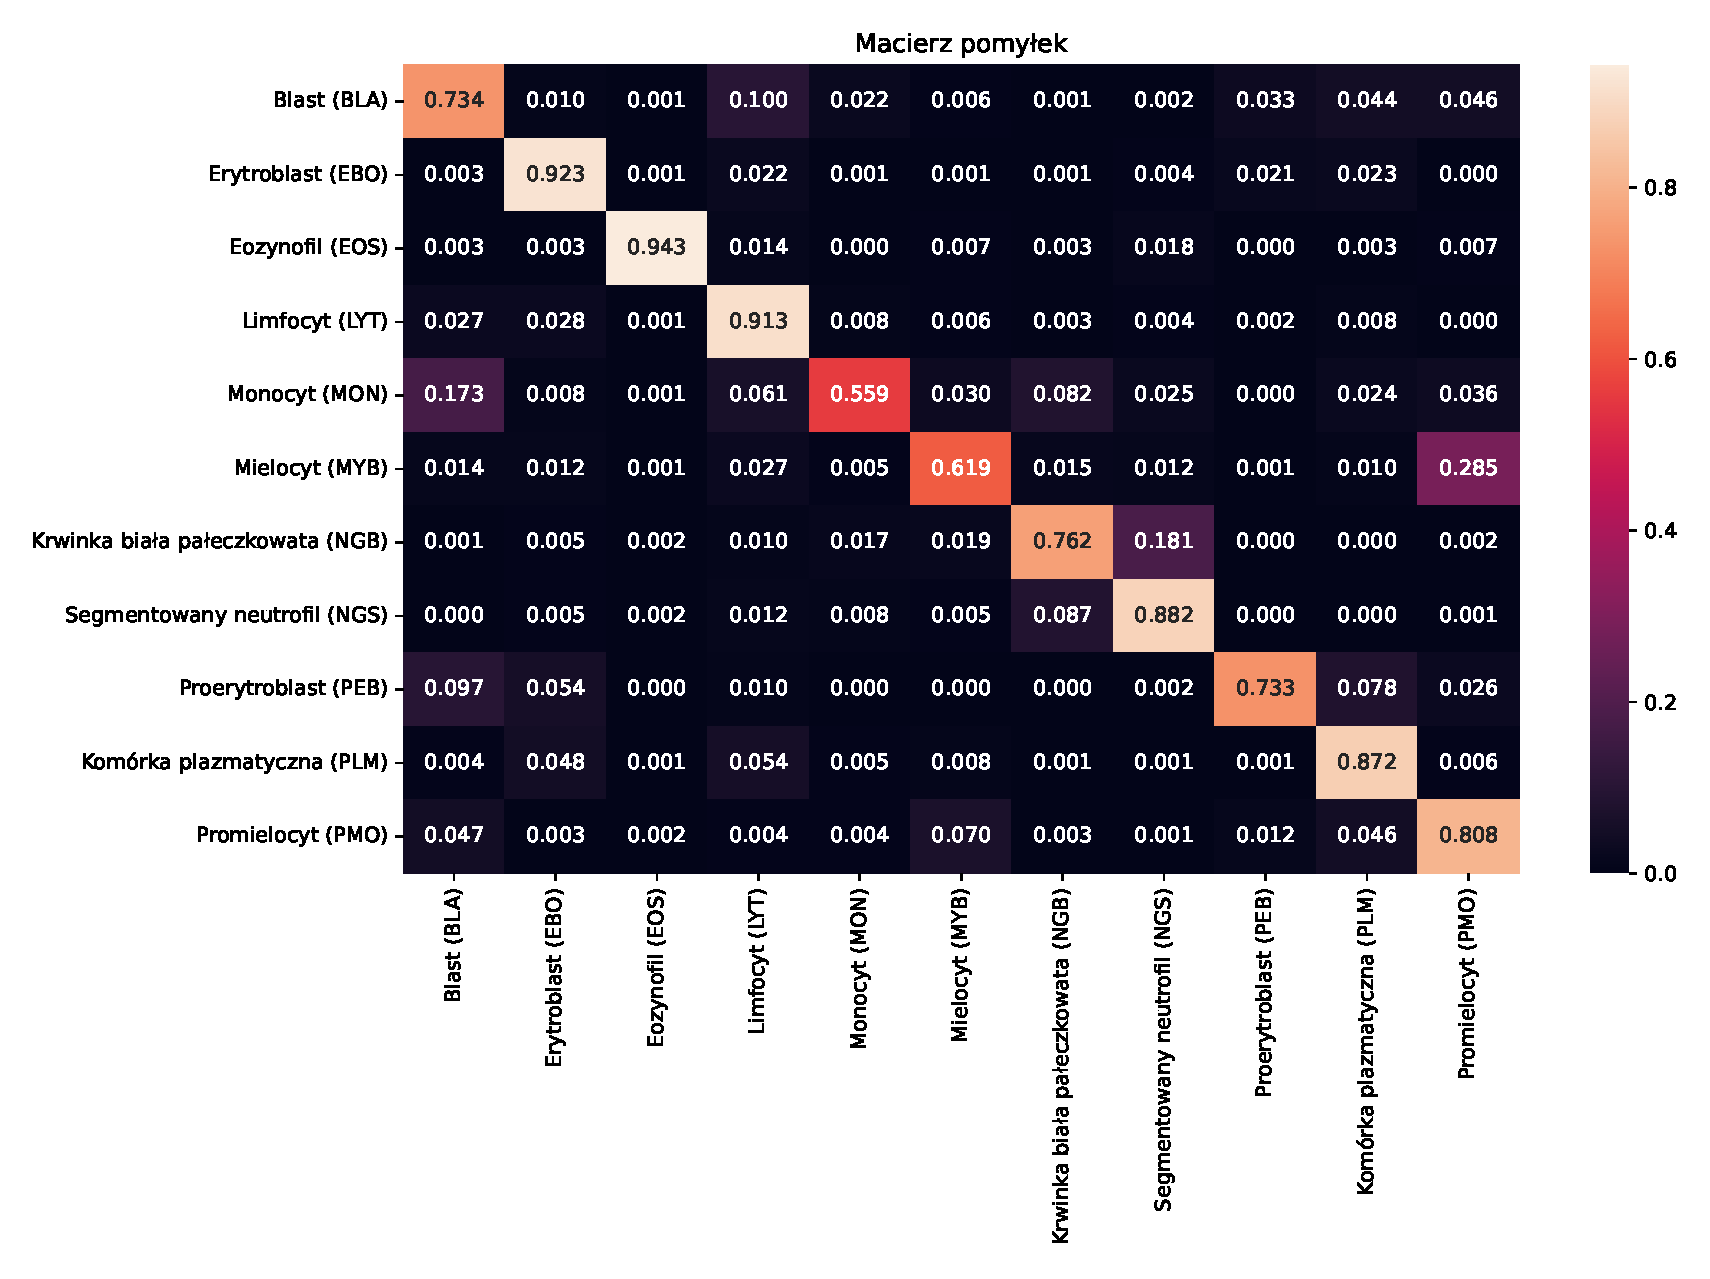
\includegraphics[width=0.8\textwidth]{experiments/resnet18/confusion_matrix}
    \caption{Macierz pomyłek modelu ResNet18}
    \label{fig:confusion_resnet18}
\end{figure}

%TODO end 9 listings


%TODO choose best architecture
Najlepsze wyniki uzyskuje model używający architektury \textit{EfficientNet B0}. Ważony wynik F1 w jej przypadku wynosi \textit{0.86}.
Tabela \ref{tab:f1_summary} przedstawia zestawienie precyzji, czułości i F1 dla poszczególnych klas.
Z kolei wykresy na rys. \ref{fig:plot} przedstawiają zależności funkcji straty i F1 od epoki trenowania.
Można stwierdzić, że jakość modelu nie poprawia się zbyt znacząco wraz z kolejnymi iteracjami.
Macierz pomyłek jest widoczna natomiast na rys. \ref{fig:confusion_matrix}.
Informuje ona, które klasy są najczęściej mylone z którymi.


\section{Porównanie z innymi algorytmami}

\begin{figure}
    \centering
    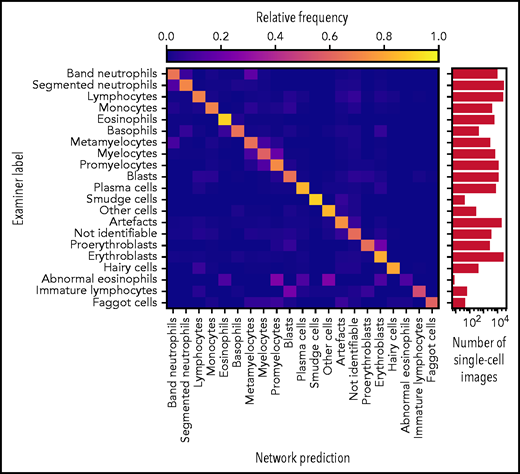
\includegraphics[width=\textwidth]{resnext_confusion_matrix}
    \caption{Macierz pomyłek dla modelu ResNeXt}
    \label{fig:resnext_confusion_matrix}
\end{figure}

Dostawca zbioru danych, w artykule \textit{Highly accurate differentiation of bone marrow cell morphologies using deep neural networks on a large image dataset} \cite{resnext} wykorzystuje architekturę \textit{ResNetXt-50}.
Model zawierający ponad 23 miliony parametrów był trenowany na \textit{NVIDIA TESLA V100} przez ok. 48 godzin.
Podobnie jak w niniejszej pracy, autorzy artykułu wykonali normalizację intensywności kolorów przed trenowaniem sieci neuronowej (z powodu różnic w barwieniu Maya-Grünwalda-Giemsa).
Uzyskany ważony wynik F1 dla architektury \textit{ResNeXt-50} wyniósł \textit{0.822}. Macierz pomyłek dostarczona przed autorów pracy jest widoczna na rys. \ref{fig:resnext_confusion_matrix}.


\section{Wyzwania}

Głównym wyzwaniem napotkanym w projekcie było wytrenowanie dużych sieci neuronowych. Niestety, ich trening na lokalnym sprzęcie takim jak komputer osobisty jest bardzo czasochłonne.
W związku z tym konieczne było uruchamianie ich na platformie \textit{kaggle.com}, która oferuje 30 godzin czasu procesora graficznego miesięcznie.
Ten górny limit wymuszał przemyślane zarządzanie tym, która sieć neuronowa powinna być wytrenowana priorytetowo.


\section{Wnioski}

%TODO net
Zaprezentowane porównanie różnych splotowych sieci neuronowych informuje, że najlepszym modelem do zadania klasyfikacji rodzajów komórek w szpiku kostnym jest \textit{EfficientNet B0}.
Ta sieć neuronowa uzyskuje najlepszy ważony wynik F1 równy \textit{0.866}.
Warto też zwrócić uwagę na to, że sieci neuronowe znacznie większe od \textit{EfficientNet B0} nie dawały dużo lepszych rezultatów.


\section{Perspektywy rozwoju projektu}

Jedną z możliwości poprawienia jakości modelu jest zrównoważenie zbioru danych, by każda z klas zawierała podobną, dużą ilość próbek.


    \chapter{Podsumowanie}

W niniejszym projekcie inżynierskim omówiono realizację systemu \textcolor{red}{klasyfikującego} rodzajów komórek szpiku kostnego \textcolor{red}{za pomocą} uczenia maszynowego.
Porównane zostały różne architektury splotowych sieci neuronowych.
Architekturą, która daje najlepsze rezultaty okazała się \textbf{EfficientNet B4}.
Przedstawione rozwiązanie oferuje podobną jakość klasyfikacji (\textcolor{red}{na podstawie} ważonej miary F1) jak \textcolor{red}{opublikowana wcześniej praca naukowa autorstwa dostawcy danych}.
Warto zauważyć jednak, że sieć EfficientNet B4 dostarcza podobnej jakości predykcji jak omawiana w innych artykułach architektura \textit{ResNeXt}, pomimo znacznie mniejszej ilości parametrów do optymalizacji (19 milionów parametrów w przypadku EfficientNet B4 w \textcolor{red}{stosunku do} 25 milionów w przypadku ResNeXt \cite{resnext}).

Opisano również algorytm ekstrakcji obrazów komórek z dużego skanu rozmazu, dzięki któremu można automatycznie wyznaczyć dane wejściowe do sieci neuronowej (sieć neuronowa wymaga obrazu pojedynczej komórki).
Do jego opracowania wykorzystano takie metody \textcolor{red}{przetwarzania obrazów} jak progowanie, znajdowanie konturów czy momenty Hu.

W ramach projektu stworzono również przejrzysty interfejs użytkownika, który umożliwia użytkownikowi łatwą interakcję z modelem sztucznej inteligencji.
Po wysłaniu obrazu komórki na serwer pojawia się tabela rozkładu prawdopodobieństwa \textcolor{red}{ rozpoznania poszczególnych klas} wraz z wizualizacją mapy cieplnej \textit{GradCam}.
Mapa cieplna pozwala użytkownikowi lepiej zrozumieć proces predykcji klas.

Podsumowując, zaprezentowany system stanowi przykład praktycznego zastosowania uczenia maszynowego i splotowych sieci neuronowych w medycynie.
W świetle obecnego tempa rozwoju technik sztucznej inteligencji, można się spodziewać, że w przyszłości rozwiązania oparte o SI będą rozwiązywały coraz bardziej złożone problemy w wielu branżach i dziedzinach życia.
Szeroko pojęta automatyzacja, napędzana przez sztuczną inteligencję, będzie prowadziła do przyspieszenia różnych procesów oraz oszczędności wielu godzin pracy specjalistów.

    % itd.
    % \appendix
    % \include{dodatekA}
    % \include{dodatekB}
    % itd.

    \printbibliography

\end{document}
